\documentclass[12pt,a4paper]{report}
\renewcommand{\baselinestretch}{1.5}
\usepackage[T1]{fontenc}
\usepackage[utf8]{inputenc}
\usepackage{times}
\usepackage{subcaption}
\usepackage{setspace}
\usepackage{multirow}
\usepackage{multicol}
\usepackage[tableposition=top]{caption}
\usepackage[table,xcdraw]{xcolor}
\usepackage{titlesec}
\usepackage{indentfirst}
\usepackage{enumitem}
\usepackage{tikz}
\usepackage{booktabs}
\usepackage{amsmath,amssymb}
\usepackage{float}
\usepackage{graphicx}
\usepackage{hyperref}
\hypersetup{
    colorlinks=true,
    linkcolor=black,
    citecolor=black,
    urlcolor=blue,
    filecolor=black
}
\usepackage[a4paper,top=40mm,bottom=30mm,left=40mm,right=30mm]{geometry}

\setlength{\parindent}{1cm}

\captionsetup[table]{labelsep=period}
\captionsetup[figure]{labelsep=period}

\usetikzlibrary{shapes.geometric, arrows, positioning, fit}

\renewcommand{\chaptername}{BAB }
\renewcommand{\figurename}{Gambar}
\renewcommand{\tablename}{Tabel}
\renewcommand{\contentsname}{DAFTAR ISI}
\renewcommand{\listtablename}{DAFTAR TABEL}
\renewcommand{\listfigurename}{DAFTAR GAMBAR}
\renewcommand{\bibname}{DAFTAR PUSTAKA}

\renewcommand{\thechapter}{\Roman{chapter}}
\renewcommand{\thesection}{\arabic{chapter}.\arabic{section}.}
\renewcommand{\thesubsection}{\arabic{chapter}.\arabic{section}.\arabic{subsection}.}
\renewcommand{\thesubsubsection}{\arabic{chapter}.\arabic{section}.\arabic{subsection}.\arabic{subsubsection}.}

\renewcommand{\thefigure}{\arabic{chapter}.\arabic{figure}}
\renewcommand{\thetable}{\arabic{chapter}.\arabic{table}}
\renewcommand{\theequation}{\arabic{chapter}.\arabic{equation}}

\usepackage{tocloft}
\renewcommand{\cfttoctitlefont}{\hspace*{\fill}\Large\bfseries}
\renewcommand{\cftaftertoctitle}{\hspace*{\fill}}
\renewcommand{\cftlottitlefont}{\hspace*{\fill}\Large\bfseries}
\renewcommand{\cftafterlottitle}{\hspace*{\fill}}
\renewcommand{\cftloftitlefont}{\hspace*{\fill}\Large\bfseries}
\renewcommand{\cftafterloftitle}{\hspace*{\fill}}
\renewcommand{\cftchapleader}{\cftdotfill{\cftchapdotsep}}
\renewcommand{\cftchapdotsep}{\cftdotsep}

\usepackage{sectsty}
\chapternumberfont{\Large}
\chaptertitlefont{\Large}
\sectionfont{\normalsize}
\subsectionfont{\normalsize}

\titleformat{\section}{\large\bfseries}{\thesection}{1em}{}
\titlespacing\section{0pt}{12pt plus 4pt minus 2pt}{0pt plus 2pt minus 2pt}
\titlespacing\subsection{0pt}{12pt plus 4pt minus 2pt}{0pt plus 2pt minus 2pt}
\titlespacing\subsubsection{0pt}{12pt plus 4pt minus 2pt}{0pt plus 2pt minus 2pt}

\titleformat{\chapter}[display]
    {\normalfont\large\bfseries\centering}{\chaptertitlename \thechapter \centering}{-10pt}{\large}
\titlespacing*{\chapter}{0pt}{-20pt}{20pt}

\setcounter{secnumdepth}{4}
\setcounter{tocdepth}{4}

\usepackage{listings}
\definecolor{codegreen}{rgb}{0,0.6,0}
\definecolor{codegray}{rgb}{0.5,0.5,0.5}
\definecolor{codepurple}{rgb}{0.58,0,0.82}
\definecolor{backcolour}{rgb}{0.97,0.97,0.97}

\lstdefinestyle{mystyle}{
    backgroundcolor=\color{backcolour},
    commentstyle=\color{codegreen},
    keywordstyle=\color{blue}\bfseries,
    numberstyle=\tiny\color{codegray},
    stringstyle=\color{codepurple},
    basicstyle=\ttfamily\footnotesize,
    breakatwhitespace=false,
    breaklines=true,
    captionpos=b,
    keepspaces=true,
    numbers=left,
    numbersep=5pt,
    showspaces=false,
    showstringspaces=false,
    showtabs=false,
    tabsize=2
}
\lstset{style=mystyle}

\begin{document}

% --- HALAMAN PRELIMINER ---
\pagenumbering{roman}
\thispagestyle{empty}
\begin{center}
    \fontsize{14pt}{18pt}\selectfont\textbf{LAPORAN KERJA MANDIRI TERPANTAU}\\[0.6cm]

    \fontsize{13pt}{17pt}\selectfont\textbf{RANCANG BANGUN SISTEM VISI KOMPUTER TERTANAM BERBASIS RASPBERRY PI 5 UNTUK KENDALI ROBOT 4-DOF: TELEOPERASI DOBOT MAGICIAN DAN PENGENALAN SIBI PADA MEARM}\\[0.6cm]

    \fontsize{11pt}{15pt}\selectfont\textit{Laporan ini Disusun Guna Memenuhi Salah Satu Persyaratan\\Menempuh Mata Kuliah Kerja Mandiri Terpantau}\\[0.8cm]

    
\includegraphics[width=3.8cm, keepaspectratio]{Gambar/uin_logo.png}\\[0.8cm]

    \fontsize{12pt}{16pt}\selectfont
    \textbf{Fahry Rizky Samsudin}\\
    \textbf{1237030018}\\[1cm]

    \textbf{JURUSAN FISIKA}\\
    \textbf{FAKULTAS SAINS DAN TEKNOLOGI}\\
    \textbf{UNIVERSITAS ISLAM NEGERI SUNAN GUNUNG DJATI BANDUNG}\\
    \textbf{2026}
\end{center}
\newpage


\setstretch{1.5}
\chapter*{\centering SURAT PERNYATAAN KEASLIAN}
\addcontentsline{toc}{chapter}{SURAT PERNYATAAN KEASLIAN}

\vspace{0.5cm}
\noindent Saya yang bertanda tangan di bawah ini:

\vspace{0.3cm}
\begin{center}
\begin{tabular}{ll}
Nama    & : Fahry Rizky Samsudin \\
NIM     & : 1237030018 \\
Jurusan & : Fisika \\
\end{tabular}
\end{center}

\vspace{0.5cm}
\noindent Dengan ini saya menyatakan sebagai berikut:
\begin{enumerate}[label=\arabic*.]
    \item Laporan Kerja Mandiri Terpantau berjudul ``Rancang Bangun Sistem Visi Komputer Tertanam Berbasis Raspberry Pi 5 untuk Kendali Robot 4-DOF: Teleoperasi Dobot Magician dan Pengenalan SIBI pada meArm'' ini merupakan hasil karya pribadi.
    \item Karya tulis ini sepenuhnya merupakan hasil pemikiran, perumusan, dan penelitian saya sendiri, dengan pengecualian berupa arahan dosen, diskusi bersama rekan, serta masukan dari pembimbing.
    \item Segala isi karya tulis ini bukan merupakan karya atau pendapat orang lain yang telah dipublikasikan, kecuali yang telah disertai dengan keterangan sumber secara jelas.
\end{enumerate}

\vspace{2cm}
\begin{flushright}
\begin{tabular}{c}
Bandung, 21 Mei 2026\\
Yang membuat pernyataan,\\[2.5cm]
\textbf{Fahry Rizky Samsudin}\\
NIM. 1237030018
\end{tabular}
\end{flushright}
\newpage

\chapter*{\centering LEMBAR PERSETUJUAN}
\addcontentsline{toc}{chapter}{LEMBAR PERSETUJUAN}

\vspace{0.3cm}
\begin{center}
    Laporan kerja mandiri terpantau\\
    \textbf{``Rancang Bangun Sistem Visi Komputer Tertanam Berbasis Raspberry Pi 5 untuk Kendali Robot 4-DOF: Teleoperasi Dobot Magician dan Pengenalan SIBI pada meArm''}\\[0.8cm]
    
    \textbf{Fahry Rizky Samsudin}\\
    \textbf{1237030018}\\[1cm]

    Menyetujui,\\[0.5cm]
    
    \begin{tabular}{cc}
        \textbf{Pembimbing I} & \textbf{Pembimbing II} \\[0.3cm]
        \begin{minipage}[c][2.2cm][c]{6cm}
            \centering
            
\includegraphics[height=1.8cm, keepaspectratio]{Gambar/ttd_pembimbing1_subkhi.png}
        \end{minipage}
        & 
        \begin{minipage}[c][2.2cm][c]{6cm}
            \centering
            
\includegraphics[height=1.8cm, keepaspectratio]{Gambar/ttd_pembimbing2_agung.png}
        \end{minipage} \\[0.2cm]
        \textbf{\underline{Dr. Moch Nurul Subkhi, M.Si}} & \textbf{\underline{Dr. Emmanuel Agung N, S.T, M.T.}} \\
        NIP. 19810201 200912 1003 & NIDN. 0407047801
    \end{tabular}
    
    \vspace{1.5cm}
    Mengetahui,\\
    \textbf{Ketua Jurusan Fisika}\\
    \textbf{Fakultas Sains dan Teknologi}\\
    \textbf{Universitas Islam Negeri Sunan Gunung Djati Bandung}\\[2.2cm]
    \textbf{\underline{Mada Sanjaya W.S., M.Si., Ph.D.}}\\
    NIP. 19851101 200912 1005
\end{center}
\newpage

\chapter*{\centering LEMBAR PENGESAHAN}
\addcontentsline{toc}{chapter}{LEMBAR PENGESAHAN}

\vspace{0.5cm}
\noindent Laporan Kerja Mandiri Terpantau dengan judul: \textbf{``Rancang Bangun Sistem Visi Komputer Tertanam Berbasis Raspberry Pi 5 untuk Kendali Robot 4-DOF: Teleoperasi Dobot Magician dan Pengenalan SIBI pada meArm''} milik Fahry Rizky Samsudin dengan NIM 1237030018 telah dipertanggungjawabkan dalam sidang Kerja Mandiri Terpantau (KMT) Jurusan Fisika Fakultas Sains dan Teknologi Universitas Islam Negeri Sunan Gunung Djati Bandung pada tanggal 19 September 2026.

\vspace{1.5cm}
\begin{center}
    Mengesahkan,\\[0.5cm]
    \textbf{Penguji Sidang}\\[2.5cm]
    \textbf{\underline{Dr. Moch Nurul Subkhi, M.Si}}\\
    NIP. 19810201 200912 1003

    \vspace{2cm}
    Mengetahui,\\
    \textbf{Ketua Jurusan Fisika}\\[2.5cm]
    \textbf{\underline{Mada Sanjaya W.S., M.Si., Ph.D.}}\\
    NIP. 19851101 200912 1005
\end{center}
\newpage

\chapter*{\centering ABSTRAK}
\addcontentsline{toc}{chapter}{ABSTRAK}

\begin{center}
\setstretch{1.2}
\begin{tabular}{ll}
Nama          & : Fahry Rizky Samsudin \\ 
Program Studi & : Fisika \\ 
Judul         & : \begin{tabular}[t]{@{}l@{}}Rancang Bangun Sistem Visi Komputer Tertanam Berbasis\\Raspberry Pi 5 untuk Kendali Robot 4-DOF: Teleoperasi\\Dobot Magician dan Pengenalan SIBI pada meArm\end{tabular} \\ 
\end{tabular}
\end{center}

\vspace{0.8cm}
\begin{spacing}{1.25}
\noindent Penelitian ini berfokus pada perancangan sistem tertanam berbasis Raspberry Pi 5 untuk kendali dua platform robot manipulator 4-DOF, yaitu Dobot Magician dan meArm. Sistem dirancang dalam dua mode kerja: mode teleoperasi untuk mengendalikan gerak Dobot Magician berdasarkan pelacakan tangan, serta mode pengenalan Sistem Isyarat Bahasa Indonesia (SIBI) untuk memetakan isyarat tangan menjadi respons gerak pada meArm. Metode yang digunakan meliputi studi literatur, integrasi perangkat keras, pengembangan piranti lunak berbasis Python 3.9, ekstraksi landmark tangan menggunakan MediaPipe, pemetaan koordinat citra ke ruang kerja robot, serta pengujian akurasi klasifikasi, presisi posisi, dan waktu respons. Laporan ini diharapkan menjadi dasar pengembangan sistem kendali robot yang ringan, portabel, dan mampu berjalan pada perangkat komputasi tepi untuk kebutuhan edukasi robotika, interaksi manusia--robot, dan pengenalan bahasa isyarat.

\vspace{0.5cm}
\noindent\textbf{Kata kunci:} Raspberry Pi 5, sistem tertanam, MediaPipe, SIBI, robot manipulator 4-DOF.
\end{spacing}
\newpage

\chapter*{\centering ABSTRACT}
\addcontentsline{toc}{chapter}{ABSTRACT}

\begin{center}
\setstretch{1.2}
\begin{tabular}{ll}
Name          & : Fahry Rizky Samsudin \\ 
Study Program & : Physics \\ 
Title         & : \begin{tabular}[t]{@{}l@{}}Design and Development of a Raspberry Pi 5-Based Embedded\\Computer Vision System for 4-DOF Robot Control: Teleoperation\\of Dobot Magician and SIBI Recognition on meArm\end{tabular} \\ 
\end{tabular}
\end{center}

\vspace{0.8cm}
\begin{spacing}{1.25}
\noindent\textit{This research focuses on designing a Raspberry Pi 5-based embedded system for controlling two 4-DOF robotic manipulator platforms, namely Dobot Magician and meArm. The system is designed with two operating modes: a teleoperation mode for controlling Dobot Magician based on hand tracking, and a recognition mode for the Indonesian Sign System (SIBI) that maps hand gestures into meArm motion responses. The method consists of literature study, hardware integration, Python 3.9-based software development, hand landmark extraction using MediaPipe, mapping of image coordinates into robot workspace coordinates, and evaluation of classification accuracy, spatial precision, and response time. This report is expected to provide a foundation for developing a lightweight and portable robotic control system that can run on edge computing devices for robotics education, human--robot interaction, and sign language recognition.}

\vspace{0.5cm}
\noindent\textbf{Keywords:}\textit{Raspberry Pi 5, embedded system, MediaPipe, SIBI, 4-DOF robotic manipulator.}
\end{spacing}
\newpage

\chapter*{\centering KATA PENGANTAR}
\addcontentsline{toc}{chapter}{KATA PENGANTAR}

\vspace{0.5cm}
Puji syukur selalu terpanjat kehadirat Allah SWT atas segala rahmat, petunjuk, dan kesempatan yang diberikan sehingga penulis dapat menyelesaikan laporan LAPORAN KERJA MANDIRI TERPANTAU dengan judul \textbf{``Rancang Bangun Sistem Visi Komputer Tertanam Berbasis Raspberry Pi 5 untuk Kendali Robot 4-DOF: Teleoperasi Dobot Magician dan Pengenalan SIBI pada meArm''}.

Penulis menghaturkan terima kasih dan apresiasi kepada seluruh pihak yang telah berkontribusi positif terhadap penulis. Ucapan terima kasih penulis haturkan kepada:
\begin{enumerate}[label=\arabic*.]
    \item Allah Subhanahu Wa Ta'ala, karena atas nikmat, karunia, dan izin-Nya, alhamdulillah laporan ini selesai disusun.
    \item Kedua orang tua dan keluarga penulis atas doa, dukungan, dan kasih sayang yang tulus.
    \item Mada Sanjaya W.S., M.Si., Ph.D., selaku Ketua Jurusan Fisika, Fakultas Sains dan Teknologi, Universitas Islam Negeri Sunan Gunung Djati Bandung.
    \item Dr. Moch Nurul Subkhi, M.Si dan Dr. Emmanuel Agung N, S.T, M.T., selaku pembimbing yang telah memberikan arahan, ilmu, serta bimbingan selama kegiatan berlangsung.
\end{enumerate}

Dengan penuh kerendahan hati, penulis menyadari bahwa laporan ini masih jauh dari sempurna dan memiliki berbagai keterbatasan. Oleh karena itu, penulis sangat mengharapkan kritik serta saran yang membangun. Semoga laporan ini dapat memberikan manfaat bagi pengembangan ilmu pengetahuan, teknologi, serta pihak-pihak yang memerlukannya.

\vspace{1.5cm}
\begin{flushright}
\begin{tabular}{c}
Bandung, 21 Mei 2026\\[1.5cm]
\textbf{Fahry Rizky Samsudin}\\
NIM. 1237030018
\end{tabular}
\end{flushright}
\newpage

\renewcommand*\contentsname{\hfill DAFTAR ISI \hfill}
\tableofcontents
\addcontentsline{toc}{chapter}{DAFTAR ISI}
\newpage

\renewcommand*\listfigurename{\hfill DAFTAR GAMBAR \hfill}
\listoffigures
\addcontentsline{toc}{chapter}{DAFTAR GAMBAR}
\newpage

\renewcommand*\listtablename{\hfill DAFTAR TABEL \hfill}
\listoftables
\addcontentsline{toc}{chapter}{DAFTAR TABEL}
\newpage


% --- NASKAH UTAMA ---
\newpage
\pagenumbering{arabic}
\chapter{PENDAHULUAN}

\section{Latar Belakang}
Perkembangan teknologi otomasi dan robotika saat ini telah mendorong transisi sistem manufaktur dan industri menuju era sistem cerdas \cite{craig2018}. Lengan robot manipulator, khususnya dengan kebebasan empat derajat (\textit{4-Degree of Freedom} atau 4-DOF), menjadi salah satu instrumen utama yang banyak diaplikasikan karena kemampuannya dalam melakukan tugas spasial seperti pemindahan barang (\textit{pick and place}), perakitan, dan inspeksi. Namun, antarmuka manusia dan mesin (\textit{Human-Machine Interface}/HMI) yang konvensional umumnya masih bergantung pada perangkat keras mekanis seperti \textit{joystick} atau pemrograman berbasis \textit{pendant}, yang membatasi fleksibilitas dan intuisi operator dalam mengendalikan pergerakan robot secara alami \cite{rautaray2015}.

Seiring dengan pesatnya kemajuan di bidang kecerdasan buatan, visi komputer (\textit{computer vision}) hadir sebagai solusi antarmuka nirsentuh (\textit{contactless}) yang lebih intuitif. Daripada memproses citra piksel mentah yang membebani komputasi, gerakan anggota tubuh manusia dapat diterjemahkan secara efisien melalui ekstraksi fitur geometris persendian (\textit{landmark extraction}) secara \textit{real-time}. Pengimplementasian sistem klasifikasi berbasis titik koordinat ini pada level perangkat keras kini dapat dilakukan menggunakan sistem tertanam (\textit{embedded system}) seperti Raspberry Pi 5. Komputasi tepi (\textit{edge computing}) pada mikrokontroler canggih ini memungkinkan eksekusi inferensi \textit{Deep Neural Networks} (DNN) berbobot ringan secara lokal, sehingga mengurangi latensi dan ketergantungan pada komputer berspesifikasi tinggi, sekaligus menjaga efisiensi daya dan ruang kerja (\textit{workspace}) \cite{shi2016}.

Meskipun demikian, tantangan utama dalam implementasi kendali visual terletak pada perhitungan mekanika terapan dan translasi spasialnya. Data visual dari kamera berwujud piksel 2D atau perkiraan kedalaman 3D, yang harus dikonversi dengan presisi tinggi ke dalam sistem koordinat fisik $(X,Y,Z)$ melalui penyelesaian persamaan kinematika robot \cite{craig2018}. Oleh karena itu, diperlukan pendekatan komputasi yang andal untuk mengelola jenis kendali mekanik yang berbeda, baik itu kendali diskret (berupa perintah spesifik) maupun kendali kontinu (pelacakan gerak dinamis) \cite{lugaresi2019}.

Untuk menjawab tantangan tersebut, penelitian ini merancang sistem kendali visual multi-mode pada manipulator 4-DOF. Pendekatan pertama menggunakan Sistem Isyarat Bahasa Indonesia (SIBI) sebagai kendali instruksional berbasis pengenalan pola abjad, yang diimplementasikan pada purwarupa robot meArm. Pendekatan kedua menggunakan pelacakan gerak tangan (\textit{hand tracking}) MediaPipe untuk teleoperasi, di mana pergeseran \textit{landmark} tangan dipetakan secara kontinu menjadi pergerakan spasial pada robot edukasi industri Dobot Magician. Pengujian terhadap kedua metode ini bertujuan untuk menganalisis respons kinematis dan keandalan sistem tertanam dalam menjalankan fungsi kontrol antar perangkat keras yang berbeda.

Berdasarkan latar belakang tersebut, penelitian ini mengangkat judul \textbf{``Rancang Bangun Sistem Visi Komputer Tertanam Berbasis Raspberry Pi 5 untuk Kendali Robot 4-DOF: Teleoperasi Dobot Magician dan Pengenalan SIBI pada meArm''}. Penelitian ini penting karena menggabungkan sistem tertanam, komputasi tepi, visi komputer, pengenalan SIBI, dan kendali kinematika robot manipulator 4-DOF dalam satu rancangan terpadu. Hasil penelitian diharapkan dapat menjadi dasar pengembangan sistem interaksi manusia--robot yang portabel, edukatif, dan dapat dikembangkan lebih lanjut untuk kebutuhan pembelajaran robotika maupun teknologi bantu komunikasi.

\section{Rumusan Masalah}
Berdasarkan latar belakang yang telah diuraikan, rumusan masalah dalam penelitian ini adalah sebagai berikut:
\begin{enumerate}[label=\arabic*.]
    \item Bagaimana merancang dan mengimplementasikan sistem visi komputer tertanam (\textit{embedded computer vision}) menggunakan Raspberry Pi 5 untuk kendali lengan robot 4-DOF?
    \item Bagaimana menerjemahkan sistem pengenalan Sistem Isyarat Bahasa Indonesia (SIBI) menjadi sinyal kendali mekanik pada lengan robot meArm?
    \item Bagaimana memetakan ekstraksi \textit{hand landmark} dari MediaPipe menjadi pergerakan teleoperasi yang kontinu berdasarkan sistem koordinat spasial $(X,Y,Z)$ pada lengan robot Dobot Magician?
\end{enumerate}

\section{Batasan Masalah}
Agar penelitian lebih terarah, batasan masalah yang digunakan adalah sebagai berikut:
\begin{enumerate}[label=\arabic*.]
    \item Pusat komputasi utama menggunakan mikrokontroler Raspberry Pi 5 yang bertindak sebagai \textit{edge computer}, di mana seluruh pemrosesan algoritma visi komputer dilakukan secara lokal tanpa bergantung pada komputasi awan (\textit{cloud computing}).
    \item Bahasa pemrograman yang digunakan untuk membangun antarmuka visi komputer dan kalkulasi mekanika adalah Python 3.9.
    \item Perangkat keras mekanik yang dievaluasi difokuskan pada dua purwarupa lengan robot 4-DOF, yaitu meArm (untuk pengujian mode pengenalan SIBI) dan Dobot Magician (untuk pengujian mode teleoperasi dinamis).
    \item Pemrosesan visi komputer untuk ekstraksi fitur dan pergerakan tangan difokuskan menggunakan kerangka kerja (\textit{framework}) MediaPipe.
    \item Algoritma pergerakan lengan robot difokuskan pada penyelesaian persamaan kinematika (\textit{inverse/forward kinematics}) dalam ruang tiga dimensi dengan memetakan titik koordinat proyektil $(X,Y,Z)$.
\end{enumerate}

\section{Tujuan Penelitian}
Tujuan penelitian ini adalah sebagai berikut:
\begin{enumerate}[label=\arabic*.]
    \item Merancang bangun sistem antarmuka nirsentuh (\textit{contactless}) untuk mengontrol manipulator robot 4-DOF melalui pemanfaatan visi komputer berbasis sistem tertanam Raspberry Pi 5.
    \item Menguji dan menganalisis tingkat keberhasilan integrasi pengenalan SIBI sebagai metode instruksi kendali diskret pada manipulator meArm.
    \item Mengimplementasikan dan mengevaluasi respons kinematis Dobot Magician saat dikendalikan secara \textit{real-time} melalui sistem teleoperasi pelacakan tangan (\textit{hand tracking}).
\end{enumerate}

\section{Manfaat Penelitian}
Manfaat teoretis dari penelitian ini adalah memberikan gambaran integrasi antara sistem tertanam, visi komputer, dan kendali kinematika robot manipulator. Penelitian ini juga dapat menjadi rujukan awal untuk pengembangan sistem interaksi manusia dan robot berbasis kamera serta komputasi tepi (\textit{edge computing}).

Manfaat praktis dari penelitian ini adalah menyediakan rancangan sistem yang dapat digunakan dalam pembelajaran robotika, demonstrasi kendali robot berbasis gestur, serta pengembangan teknologi bantu berbasis SIBI. Selain itu, penggunaan mikrokontroler Raspberry Pi 5 menjadikan sistem relatif ringkas, hemat daya, dan mudah direplikasi pada laboratorium pendidikan.

\section{Waktu dan Tempat Penelitian}
Penelitian ini dilaksanakan pada bulan Januari hingga Februari 2026 di Laboratorium Program Studi Teknologi Mekatronika, Politeknik Enjinering Indorama (PEI), Kabupaten Purwakarta, Jawa Barat. Peralatan utama yang digunakan meliputi Raspberry Pi 5 sebagai komputasi tepi, kamera web Logitech, lengan robot Dobot Magician, dan purwarupa meArm 4-DOF.

\chapter{PROFIL INDUSTRI}

\section{Profil Politeknik Enjinering Indorama}
Politeknik Enjinering Indorama (PEI) adalah institusi pendidikan tinggi vokasi yang berlokasi di Kabupaten Purwakarta, Jawa Barat. Sesuai dengan tujuan utamanya untuk menjadi politeknik kelas dunia, PEI mengintegrasikan secara langsung pendidikan akademis berkualitas dengan pengalaman praktis di lingkungan industri. Pendekatan ini dirancang untuk menjembatani kesenjangan antara teori rekayasa dan kebutuhan nyata di lapangan kerja industri manufaktur.

Secara spesifik, pelaksanaan Kerja Praktik ini bernaung di bawah Program Studi Teknologi Mekatronika PEI. Program studi jenjang Sarjana Terapan ini menyelenggarakan pendidikan yang berfokus pada disiplin ilmu rekayasa sinergis, menggabungkan teknik mesin, elektronika, sistem kendali, dan rekayasa perangkat lunak. Laboratorium Teknologi Mekatronika PEI memiliki fasilitas tingkat lanjut yang dirancang untuk mereplikasi lingkungan manufaktur modern, menjadikannya tempat yang sangat ideal bagi mahasiswa praktikan untuk mengembangkan purwarupa otomasi dan komputasi cerdas.

\section{Sejarah Politeknik Enjinering Indorama}
PT Indo-Rama Synthetics Tbk. didirikan pada tahun 1975 dan memulai operasi komersial dengan mendirikan pabrik pemintalan kapas di Purwakarta pada tahun 1976. Perusahaan terus melakukan diversifikasi dan memperluas bisnis untuk pasar global. Indorama merupakan salah satu eksportir terbesar di Indonesia dan telah menjadi pemenang rutin penghargaan Primaniyarta yang prestisius untuk kinerja ekspornya, menjadikannya salah satu produsen poliester paling kompetitif di seluruh dunia berkat proses investasi ulang yang berkesinambungan dan program peningkatan produktivitas.

Melalui Yayasan Pendidikan Indorama, PT Indo-Rama Synthetics Tbk. memutuskan untuk mengembangkan politeknik kelas dunia yang berfokus pada penyediaan pendidikan berkualitas tinggi dan relevan dengan industri dengan biaya terjangkau. Lembaga nirlaba ini disebut Politeknik Enjinering Indorama (PEI), yang pendiriannya diselesaikan setelah dua tahun perencanaan cermat mengenai kompetensi pekerjaan dan persyaratan keterampilan industri. PEI didirikan sebagai \textit{eco-campus} di atas lahan hijau seluas 6 hektar dengan lokasi strategis yang berdekatan dengan fasilitas manufaktur Indorama.

Di dalam ekosistem kampus yang terintegrasi dengan industri ini, Program Studi Teknologi Mekatronika dibentuk secara strategis sebagai jawaban atas tantangan era Industri 4.0. Sejak didirikan, program studi ini terus mengembangkan kapasitas laboratoriumnya---mulai dari sistem pneumatik dasar hingga robotika mutakhir---untuk memastikan lulusannya siap menjadi pelopor rekayasa teknologi dan memiliki daya saing di kawasan regional.

\section{Visi dan Misi Politeknik Enjinering Indorama}
Dalam menyelenggarakan pendidikan dan riset terapan, institusi dan program studi menetapkan visi dan misi sebagai arah gerak dan standar keunggulan institusi:

\subsection{Visi Politeknik Enjinering Indorama}
Menjadi Politeknik Kelas Dunia dengan Memberikan Pendidikan Berkualitas dan Pengalaman Praktis di Industri untuk Menghasilkan Lulusan Siap Kerja.

\subsection{Misi Politeknik Enjinering Indorama}
\begin{enumerate}[label=\arabic*.]
    \item Menyelenggarakan pendidikan vokasi untuk menghasilkan sumber daya manusia yang berkualitas, memiliki keunggulan dan kemandirian, dengan didukung pengembangan kurikulum, laboratorium dan Alat Pembelajaran serta Tenaga Pengajar Berkualitas.
    \item Menyelenggarakan penelitian untuk mengembangkan ilmu pengetahuan dan teknologi guna meningkatkan kesejahteraan masyarakat.
    \item Menyelenggarakan pengabdian kepada masyarakat dan diseminasi teknologi dan hasil-hasil penelitian untuk memecahkan masalah-masalah yang ada di masyarakat.
    \item Membangun 5 kompetensi kritikal yang berhubungan dengan penyelesaian masalah, kolaborasi kerjasama tim, produktivitas, fokus dalam kualitas dan memiliki kemampuan komputer dan bahasa Inggris.
\end{enumerate}

\subsection{Visi Program Studi Teknologi Mekatronika}
Menjadi program studi vokasi terdepan yang bermitra erat dengan industri guna mengaplikasikan teknologi di bidang Mekatronika dan memenuhi kebutuhan Sumber Daya Manusia yang kompeten dan mampu yang berdaya saing dalam kawasan regional.

\subsection{Misi Program Studi Teknologi Mekatronika}
\begin{enumerate}[label=\arabic*.]
    \item Menyelenggarakan pendidikan Sarjana Terapan bidang rekayasa mekatronika, mampu menyediakan tenaga profesional yang kompeten di bidang Mekatronika.
    \item Berperan aktif menyelenggarakan penelitian dan kajian terapan dalam bidang rekayasa mekatronika.
    \item Menjalin kemitraan dan bisnis dengan industri tekstil dan industri manufaktur umum melalui rekayasa teknologi mekatronika.
    \item Menciptakan iklim kompetisi bidang rekayasa teknologi yang berwawasan wirausaha.
    \item Mengembangkan teknologi mekatronika yang dapat diaplikasikan secara langsung kepada masyarakat.
\end{enumerate}

\section{Roadmap Politeknik Enjinering Indorama}
Dalam mendukung pencapaian visi institusi dan memfasilitasi pengembangan teknologi tepat guna, Politeknik Enjinering Indorama memiliki peta jalan (\textit{roadmap}) strategis yang komprehensif. Peta jalan ini mencakup tiga pilar utama yang sangat relevan dengan fokus riset Program Studi Teknologi Mekatronika:

\begin{enumerate}[label=\arabic*.]
    \item \textbf{Roadmap Program Pendidikan dan Kurikulum}:
    \begin{itemize}
        \item \textbf{Pendidikan Vokasi Terapan}: Menyelaraskan rancangan kurikulum dengan Standar Nasional Pendidikan Tinggi (SN-Dikti) dan standar kompetensi industri global.
        \item \textbf{Fokus Program Studi}: Berkonsentrasi pada program studi berbasis rekayasa teknik dan manufaktur yang sangat dibutuhkan oleh sektor industri, di antaranya Teknologi Rekayasa Manufaktur, Teknologi Rekayasa Mekatronika, dan Teknologi Listrik.
        \item \textbf{Target Lulusan}: Menciptakan tenaga ahli vokasi yang cerdas, aktif, disiplin, religius, serta siap pakai untuk memimpin di lingkungan kerja industri modern.
    \end{itemize}
    
    \item \textbf{Roadmap Penelitian Terapan}:
    \begin{itemize}
        \item \textbf{Fokus Riset}: Penelitian di PEI diarahkan secara spesifik pada riset terapan yang mampu menjawab tantangan dan kebutuhan nyata di dunia industri, khususnya dalam bidang otomasi dan teknologi manufaktur.
        \item \textbf{Dukungan Institusi}: Kegiatan riset didukung penuh oleh Lembaga Penelitian dan Pengabdian kepada Masyarakat (LPPM) yang mengarahkan pendanaan ke riset yang berpotensi menghasilkan paten dan hilirisasi produk.
        \item \textbf{Kolaborasi Industri}: Terus memperkuat kerja sama strategis dengan mitra korporasi, termasuk PT Indo-Rama Synthetics Tbk, sebagai bagian dari program \textit{Corporate Social Responsibility} (CSR) berbasis pendidikan berkelanjutan.
    \end{itemize}
    
    \item \textbf{Rencana Strategis (Renstra) dan Akreditasi}:
    \begin{itemize}
        \item \textbf{Pencapaian Akreditasi}: Berkomitmen penuh untuk meraih dan mempertahankan akreditasi unggul dari Lembaga Akreditasi Mandiri (LAM) Teknik dan BAN-PT, guna mengukuhkan PEI sebagai institusi rujukan di Jawa Barat.
        \item \textbf{Sistem Penjaminan Mutu}: Melaksanakan proses evaluasi dan audit mutu internal secara berkala melalui Badan Penjaminan Mutu Internal (BPMI).
    \end{itemize}
\end{enumerate}

\chapter{TINJAUAN PUSTAKA}

\section{Sistem Visi Komputer Tertanam (\textit{Embedded Computer Vision})}
Sistem visi komputer tertanam (\textit{embedded computer vision}) merupakan bidang interdisipliner yang menggabungkan perangkat keras sistem tertanam (\textit{embedded system}) dengan algoritma visi komputer untuk mengeksekusi tugas pemrosesan citra secara mandiri \cite{szeliski2022}. Berbeda dengan arsitektur komputasi awan yang memproses data visual di peladen jarak jauh, sistem tertanam dirancang untuk melakukan inferensi langsung di lokasi tempat data diakuisisi. Pendekatan ini sangat krusial dalam pengendalian robotika \textit{real-time}, karena menghilangkan dependensi terhadap konektivitas jaringan eksternal dan secara dramatis memangkas waktu tunda transmisi (\textit{transmission delay}) \cite{li2018}.

Pengaplikasian visi tertanam pada robotika modern juga memberikan keuntungan signifikan dari segi desain mekanis. Karena seluruh beban komputasi visi diselesaikan oleh \textit{microcomputer} yang berdimensi kecil, sistem ini secara substansial mengurangi beban muatan (\textit{payload}) dan konsumsi daya (\textit{power consumption}) dibandingkan dengan menggunakan \textit{Personal Computer} (PC) konvensional \cite{shi2016}. Hal ini memungkinkan perancangan lengan robot manipulator yang lebih ringkas, mandiri, dan fleksibel untuk diintegrasikan ke dalam berbagai lingkungan kerja spasial tanpa memerlukan infrastruktur jaringan yang kompleks. Implementasi antarmuka sistem visi komputer tertanam pada stasiun kerja kendali Dobot Magician ditunjukkan pada Gambar \ref{fig:antarmuka_dobot}.

\begin{figure}[htbp]
    \centering
    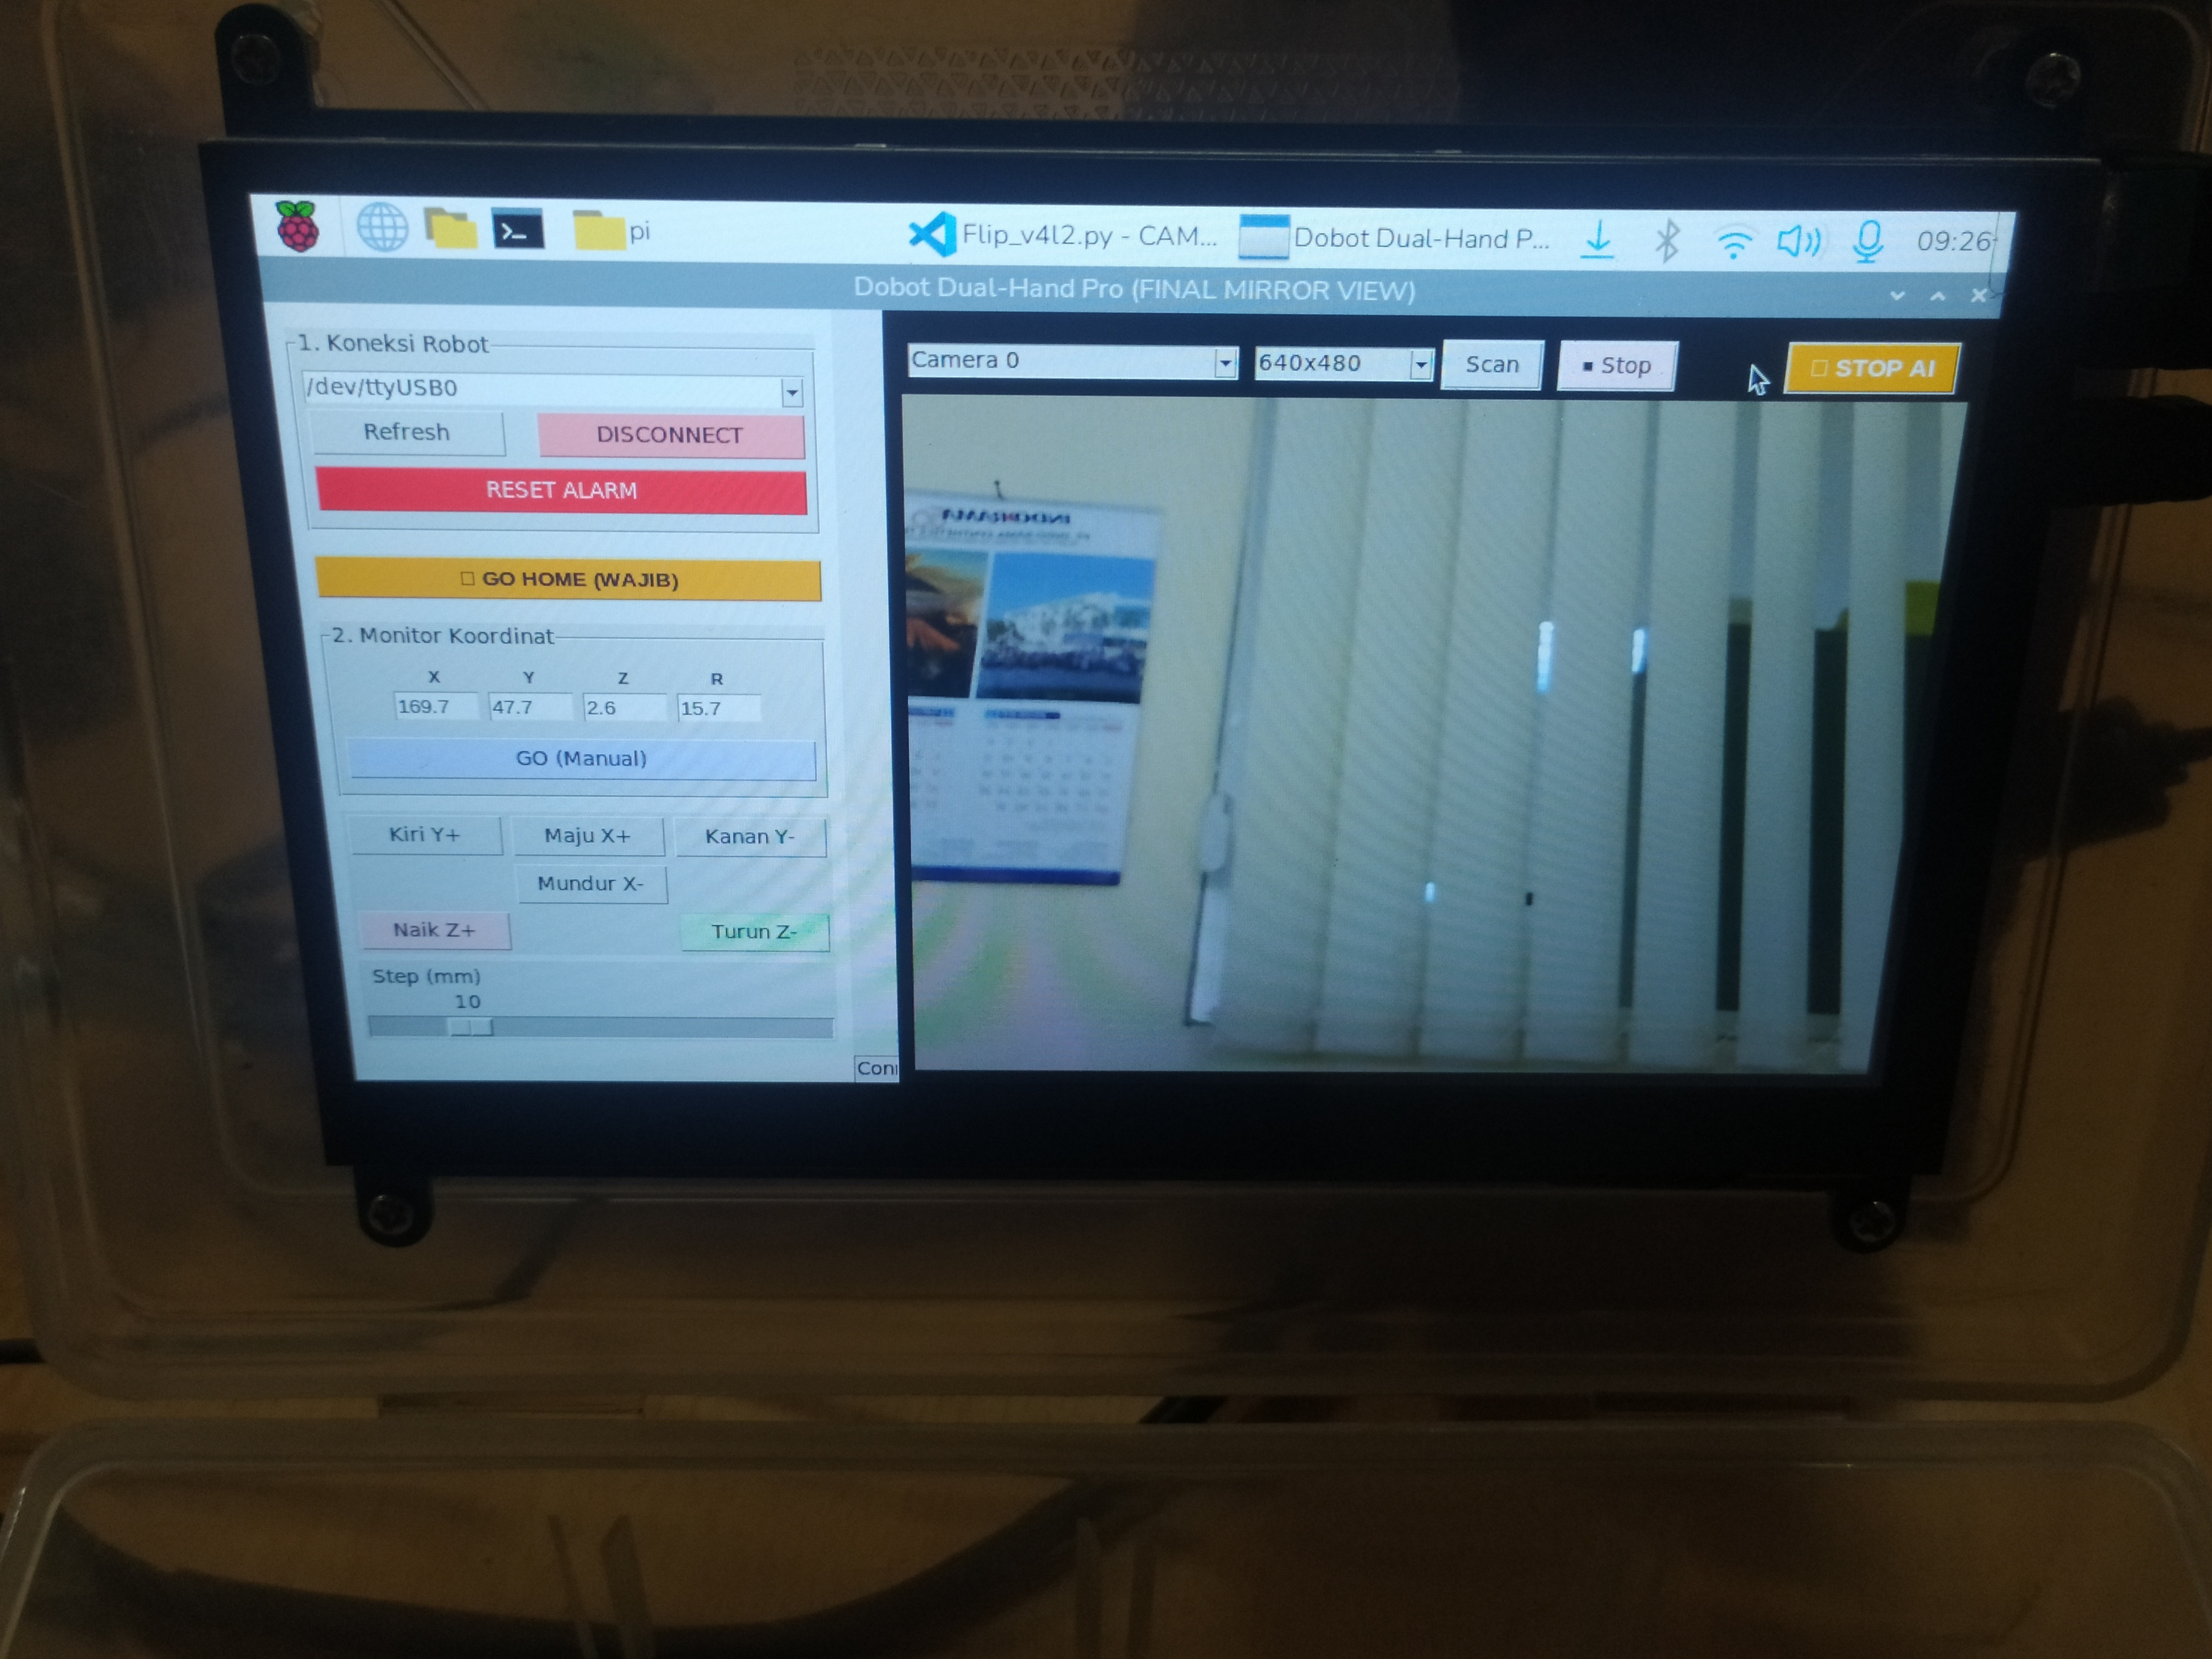
\includegraphics[width=0.85\textwidth]{Gambar/Gambar3_1_antarmuka_dobot.jpg}
    \caption{Antarmuka Sistem Visi Komputer Tertanam pada Kendali Dobot Magician}
    \label{fig:antarmuka_dobot}
\end{figure}

\section{Komputasi Tepi (\textit{Edge Computing}) dengan Raspberry Pi 5}
Komputasi tepi (\textit{edge computing}) adalah paradigma arsitektur teknologi informasi yang mendistribusikan beban kerja komputasi sedekat mungkin dengan sumber data sensorik \cite{satyanarayanan2017}. Dalam sistem robotika kendali visual, kamera bertindak sebagai node sensor berkecepatan tinggi yang terus menerus menghasilkan aliran data (\textit{data stream}). Jika aliran citra ini dikirim ke \textit{server} awan untuk diproses, akan terjadi disipasi \textit{bandwidth} yang besar dan latensi yang fluktuatif. Komputasi tepi menyelesaikan masalah ini dengan menarik kapabilitas analitik kecerdasan buatan langsung ke lapisan perangkat fisik (\textit{device layer}), memastikan waktu respons pergerakan robot berada pada batas waktu nyata (\textit{hard real-time constraints}).

Sebagai platform perangkat keras komputasi tepi, Raspberry Pi 5 ditenagai oleh \textit{System-on-Chip} (SoC) BCM2712 dengan arsitektur ARM Cortex-A76 \textit{quad-core} \cite{rpi5brief2023}. Peningkatan kinerja komputasi instruksi tunggal (\textit{single-thread}) pada mikrokontroler ini memungkinkannya untuk menjalankan model inferensi \textit{Deep Neural Networks} (DNN) dan pelacakan koordinat spasial tanpa memerlukan akselerator grafis terpisah (\textit{dedicated GPU}). Antarmuka PCIe 2.0 dan \textit{bandwidth} memori yang tinggi menjadikannya instrumen yang sangat mumpuni untuk purwarupa kendali robotika \textit{edge AI} berskala industri maupun edukasi \cite{wang2020}.

\section{Visi Komputer dan Ekstraksi Fitur Geometris (\textit{Landmark Extraction})}
Dalam sistem interaksi manusia-robot, proses pengolahan visual sering kali terkendala oleh besarnya beban komputasi apabila mengandalkan pemrosesan matriks piksel mentah \cite{rautaray2015}. Konversi dari citra warna (RGB) tiga kanal beresolusi tinggi secara langsung membutuhkan spesifikasi memori dan \textit{clock speed} yang jauh melampaui kapasitas rata-rata \textit{Single Board Computer} (SBC). Oleh karena itu, pendekatan ekstraksi fitur yang optimal untuk komputasi tepi harus beralih dari analisis piksel masif menuju pemahaman geometri struktur objek utama di dalam \textit{frame}.

Sebagai solusi efisiensi komputasi tepi, proses ekstraksi fitur difokuskan pada geometri struktur objek melalui metode \textit{landmark extraction} \cite{zhang2020}. Pada pendekatan ini, citra kasar tidak diklasifikasikan secara utuh, melainkan direduksi terlebih dahulu menjadi susunan titik-titik koordinat spasial yang merepresentasikan persendian kerangka objek (tangan). Kumpulan titik ini membentuk vektor numerik satu dimensi (1D array) yang sangat ringan. Vektor fitur spasial yang padat (\textit{dense feature vector}) inilah yang kemudian diumpankan maju (\textit{feed-forward}) ke dalam model \textit{Deep Neural Networks} (DNN) \textit{fully-connected} standar, memastikan \textit{inference time} dalam hitungan milidetik.

\section{Pengenalan Sistem Isyarat Bahasa Indonesia (SIBI) Berbasis DNN}
Sistem Isyarat Bahasa Indonesia (SIBI) merupakan tata bahasa isyarat formal yang memanfaatkan artikulasi jari-jemari tangan (\textit{dactylology}) dan posisi spasial tangan relatif terhadap tubuh untuk merepresentasikan abjad alfabet (A--Z) dan struktur numerik \cite{kosasih2012}. Setiap huruf dalam SIBI memiliki karakteristik lekukan jari dan orientasi telapak tangan yang sangat spesifik. Dalam konteks \textit{Human-Machine Interface} (HMI), variabilitas gestur ini merupakan kandidat ideal untuk digunakan sebagai pustaka instruksi mandiri (\textit{command library}), di mana setiap abjad dapat dipetakan secara eksklusif (\textit{one-to-one mapping}) pada aksi lengan robot meArm, seperti perintah buka-tutup \textit{gripper} atau transisi antar sumbu koordinat.

Dalam implementasi kendali ini, pengenalan abjad SIBI tidak menggunakan \textit{Convolutional Neural Networks} (CNN), melainkan diproses menggunakan arsitektur \textit{Deep Neural Networks} (DNN) standar \cite{goodfellow2016}. Fitur \textit{input} yang digunakan adalah nilai jarak relatif atau koordinat $(x,y,z)$ dari 21 titik persendian tangan hasil ekstraksi struktur geometris. Variasi kelengkungan jari pada formasi isyarat SIBI akan menghasilkan larik (\textit{array}) angka yang unik. DNN bertugas memodelkan probabilitas matematika dari susunan angka tersebut melalui fungsi aktivasi non-linear pada lapisan tersembunyi (\textit{hidden layers}). \textit{Output} dari lapisan akhir sistem DNN memprediksi probabilitas tertinggi dari formasi tangan untuk diklasifikasikan ke dalam instruksi spesifik (\textit{discrete control}).

\section{Pelacakan Gerak Tangan (\textit{Hand Tracking}) Menggunakan MediaPipe}
MediaPipe adalah kerangka kerja (\textit{framework}) lintas platform sumber terbuka yang dirancang oleh Google untuk membangun saluran inferensi (\textit{perception pipelines}) berbasis video dengan latensi sangat rendah \cite{lugaresi2019}. Keunggulan utama MediaPipe terletak pada kemampuannya untuk merangkai beberapa model \textit{Machine Learning} secara berurutan dalam sebuah \textit{graph} sinkron, memungkinkan eksekusi deteksi objek dinamis pada \textit{hardware} dengan spesifikasi terbatas tanpa menyebabkan \textit{bottleneck} pemrosesan.

Modul \textit{MediaPipe Hand Tracking} beroperasi menggunakan arsitektur inferensi dua tahap (\textit{two-stage architecture}) \cite{zhang2020}. Tahap pertama menggunakan algoritma detektor telapak tangan (\textit{palm detector model}) untuk melokalisasi \textit{bounding box} area tangan pada \textit{frame} gambar awal. Setelah tangan terlacak, tahap kedua menjalankan model penanda fitur (\textit{hand landmark model}) hanya pada area terpotong (\textit{cropped area}) tersebut untuk memprediksi 21 titik koordinat persendian spasial 3D $(x,y,z)$ secara presisi dan kontinu. Pendekatan prediksi berjenjang ini secara masif mereduksi beban komputasi. Koordinat inilah yang diekstrak sebagai \textit{input} larik numerik (\textit{array}) untuk model DNN pada mode pengenalan SIBI, serta digunakan sebagai target perpindahan sumbu spasial langsung pada mode teleoperasi dinamis Dobot Magician.

Topologi persebaran dan penamaan dari ke-21 titik persendian tangan tersebut diilustrasikan pada Gambar \ref{fig:mediapipe_landmarks}.

\begin{figure}[htbp]
    \centering
    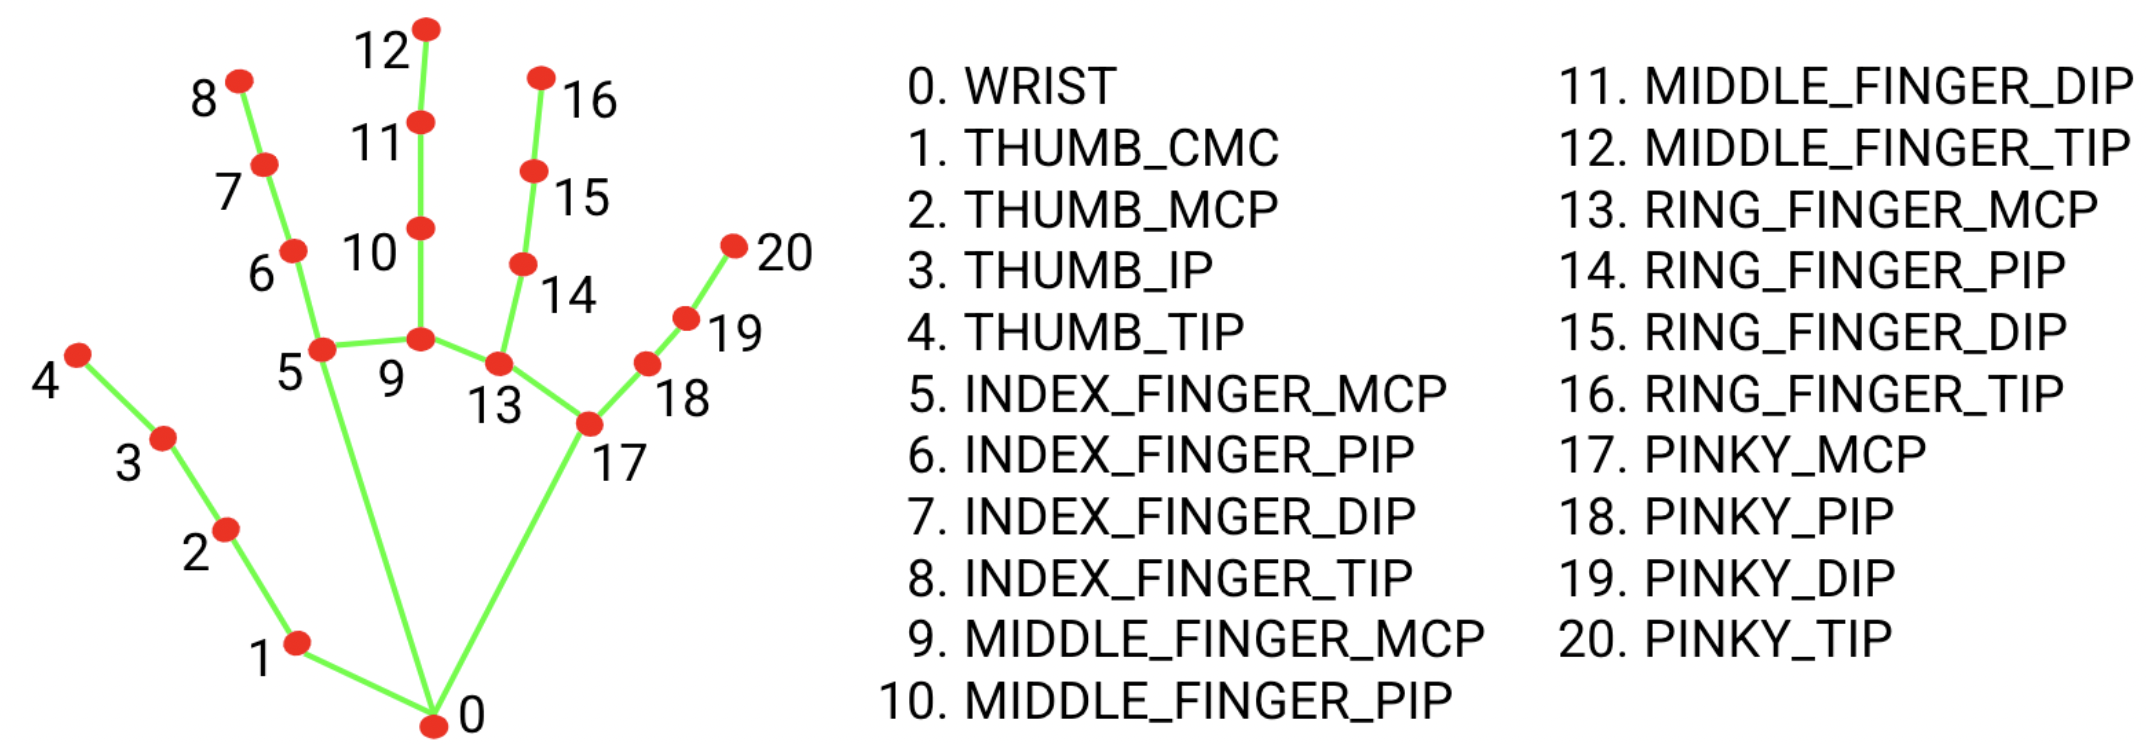
\includegraphics[width=0.85\textwidth]{Gambar/Gambar3_2_mediapipe_landmarks.png}
    \caption{Representasi 21 Titik Persendian Tangan (\textit{Hand Landmarks}) pada Framework MediaPipe}
    \label{fig:mediapipe_landmarks}
\end{figure}

Berdasarkan Gambar \ref{fig:mediapipe_landmarks}, setiap titik persendian tangan memiliki indeks anatomi spesifik, dimulai dari titik 0 yang merepresentasikan pergelangan tangan (WRIST). Titik pergelangan ini difungsikan sebagai titik acuan referensi origin $(0,0,0)$ dalam tahap normalisasi posisi spasial tangan. Titik persendian berikutnya terbagi ke dalam lima jari: ibu jari (titik 1--4: THUMB\_CMC, THUMB\_MCP, THUMB\_IP, THUMB\_TIP), jari telunjuk (titik 5--8: INDEX\_FINGER\_MCP hingga INDEX\_FINGER\_TIP), jari tengah (titik 9--12: MIDDLE\_FINGER\_MCP hingga MIDDLE\_FINGER\_TIP), jari manis (titik 13--16: RING\_FINGER\_MCP hingga RING\_FINGER\_TIP), dan kelingking (titik 17--20: PINKY\_MCP hingga PINKY\_TIP). Informasi spasial tiga dimensi $(x,y,z)$ dari seluruh titik persendian menghasilkan 63 nilai skalar fitur geometris yang merepresentasikan postur tangan secara invarian terhadap latar belakang visual.

\section{Kinematika Lengan Robot Manipulator 4-DOF}
Kinematika adalah cabang mekanika analitik yang mempelajari pergerakan murni suatu sistem benda multi-bodi tanpa mempertimbangkan gaya (torsi) maupun massa yang menyebabkan pergerakan tersebut \cite{craig2018}. Pada analisis lengan robot 4-DOF (\textit{Degree of Freedom}), sistem mekanis dimodelkan sebagai rangkaian segmen kaku (\textit{rigid links}) yang terhubung oleh persendian rotasional. Konfigurasi 4-DOF umumnya menyediakan tiga derajat kebebasan untuk translasi posisi pada koordinat spasial $(X,Y,Z)$ dan satu derajat kebebasan tambahan untuk mengontrol orientasi (\textit{pitch} sudut kemiringan) pada ujung efektor (\textit{end-effector}).

Penyelesaian matematis pergerakan ini sangat esensial dalam perancangan kendali robot dan terbagi menjadi dua penyelesaian utama, yaitu kinematika maju (\textit{forward kinematics}) dan kinematika balikan (\textit{inverse kinematics}) \cite{lynch2017}.

\subsection{Kinematika Maju (\textit{Forward Kinematics})}
Kinematika maju digunakan untuk menghitung posisi dan orientasi absolut dari \textit{end-effector} di ruang Cartesian berdasarkan besaran sudut rotasi yang diumpankan pada masing-masing motor sendi $(\theta_1, \theta_2, \theta_3, \theta_4)$. Berdasarkan pendekatan analisis geometris pada lengan robot artikulasi 4-DOF, lengan direpresentasikan dengan panjang tautan lengan atas ($L_1$), lengan bawah ($L_2$), dan tautan efektor ($L_3$). Tinggi basis dari titik tumpu dinyatakan sebagai $d_1$.

Orientasi sudut kemiringan (\textit{pitch angle}) dari \textit{end-effector} terhadap bidang horizontal disimbolkan dengan $\phi$, yang merupakan akumulasi dari rotasi sendi kedua hingga keempat:
\begin{equation}
\phi = \theta_2 + \theta_3 + \theta_4
\label{eq:phi}
\end{equation}

Posisi radius jangkauan horizontal ($r$) pada bidang proyeksi dua dimensi dirumuskan melalui penjumlahan vektor trigonometri berikut:
\begin{equation}
r = L_1 \cos(\theta_2) + L_2 \cos(\theta_2 + \theta_3) + L_3 \cos(\phi)
\label{eq:r}
\end{equation}

Berdasarkan nilai radius tersebut, proyeksi koordinat Cartesian spasial $(X,Y,Z)$ untuk posisi akhir ujung robot dapat dikalkulasi secara lengkap menggunakan himpunan persamaan:
\begin{equation}
\begin{cases}
X = r \cos(\theta_1), \\
Y = r \sin(\theta_1), \\
Z = d_1 + L_1 \sin(\theta_2) + L_2 \sin(\theta_2 + \theta_3) + L_3 \sin(\phi).
\end{cases}
\label{eq:fk}
\end{equation}
di mana $\theta_1$ mewakili sudut putar pada sendi basis (\textit{base yaw}).

\subsection{Kinematika Balikan (\textit{Inverse Kinematics})}
Kinematika balikan merupakan proses komputasi untuk mencari nilai sudut persendian $(\theta_1, \theta_2, \theta_3, \theta_4)$ yang dibutuhkan agar \textit{end-effector} mencapai target koordinat spasial $(X,Y,Z)$ dengan sudut orientasi $\phi$ tertentu \cite{craig2018}. Penyelesaian pada robot 4-DOF diuraikan dalam beberapa tahapan komputasi geometris.

Pertama, sudut putar basis ($\theta_1$) dan jarak radius planar ($r$) dihitung menggunakan fungsi tangen dua argumen dan teorema Pythagoras:
\begin{equation}
\begin{cases}
\theta_1 = \text{atan2}(Y, X), \\
r = \sqrt{X^2 + Y^2}.
\end{cases}
\label{eq:ik_theta1}
\end{equation}

Tahap kedua adalah mendekomposisi posisi \textit{end-effector} untuk menemukan koordinat persendian pergelangan atau \textit{wrist center} $(r_w, z_w)$. Titik ini merupakan ujung dari tautan $L_2$ dan pangkal dari $L_3$:
\begin{equation}
\begin{cases}
r_w = r - L_3 \cos(\phi), \\
z_w = Z - d_1 - L_3 \sin(\phi).
\end{cases}
\label{eq:wrist_center}
\end{equation}

Tahap ketiga menerapkan Hukum Kosinus pada segitiga yang dibentuk oleh $L_1$, $L_2$, dan garis hipotenusa imajiner yang menghubungkan pangkal $L_1$ dengan \textit{wrist center}. Sudut sendi siku ($\theta_3$) diselesaikan dengan persamaan:
\begin{equation}
\begin{cases}
c_3 = \dfrac{r_w^2 + z_w^2 - L_1^2 - L_2^2}{2 L_1 L_2}, \\[10pt]
\theta_3 = \text{atan2}\left(\pm \sqrt{1 - c_3^2}, c_3\right).
\end{cases}
\label{eq:ik_theta3}
\end{equation}
dengan $c_3 = \cos(\theta_3)$. Tanda $\pm$ mengindikasikan keberadaan dua solusi postur (\textit{elbow-up} atau \textit{elbow-down}).

Tahap keempat menghitung sudut sendi bahu ($\theta_2$) dengan memanfaatkan sudut dekomposisi $\alpha$ dan $\beta$:
\begin{equation}
\begin{cases}
\alpha = \text{atan2}(z_w, r_w), \\[6pt]
\beta = \text{atan2}(L_2 \sin(\theta_3), L_1 + L_2 \cos(\theta_3)), \\[6pt]
\theta_2 = \alpha - \beta.
\end{cases}
\label{eq:ik_theta2}
\end{equation}

Tahap terakhir adalah mengkalkulasi sudut sendi pergelangan ($\theta_4$) berdasarkan nilai orientasi $\phi$ yang telah ditetapkan:
\begin{equation}
\theta_4 = \phi - \theta_2 - \theta_3
\label{eq:ik_theta4}
\end{equation}

\subsection{Implementasi pada Perangkat Keras 4-DOF}
Pemodelan matematis ini diimplementasikan secara spesifik pada dua varian lengan robot 4-DOF:

\subsubsection{Dobot Magician}
Dobot Magician merupakan lengan robot industrial yang digerakkan menggunakan aktuator motor \textit{stepper} berpresisi tinggi \cite{dobot2022, dobot2026}. Kestabilan mekanisnya sangat ideal untuk mode teleoperasi dinamis, sebagaimana ditunjukkan pada Gambar \ref{fig:dobot_magician}. Pada mode ini, penyelesaian \textit{inverse kinematics} (Persamaan (\ref{eq:ik_theta1}) hingga Persamaan (\ref{eq:ik_theta4})) dieksekusi secara kontinu oleh Raspberry Pi untuk mengonversi pergeseran matriks $(x,y,z)$ dari \textit{landmark} tangan manusia menjadi matriks sudut $(\theta_1, \theta_2, \theta_3, \theta_4)$. Data sudut ini kemudian ditransmisikan ke pengendali internal robot agar mampu mereplikasi pergerakan tangan operator secara \textit{real-time}.

\begin{figure}[htbp]
    \centering
    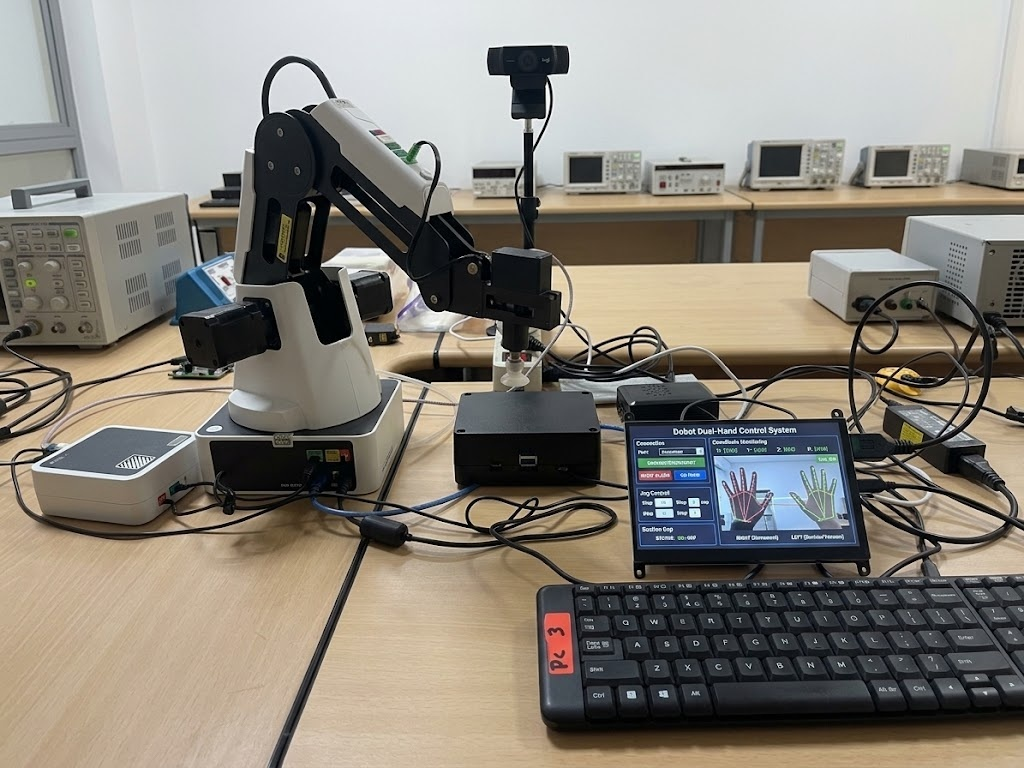
\includegraphics[width=0.75\textwidth]{Gambar/Gambar3_3_dobot_magician.jpg}
    \caption{Lengan Robot Dobot Magician untuk Implementasi Teleoperasi Dinamis}
    \label{fig:dobot_magician}
\end{figure}

\subsubsection{meArm}
meArm adalah purwarupa manipulator berskala kecil berbahan dasar akrilik yang digerakkan oleh motor servo standar \cite{mearm2026}. Konfigurasi fisik purwarupa meArm tampak depan dan tampak samping diilustrasikan pada Gambar \ref{fig:mearm_prototype}. Konfigurasi mekanis ini digunakan secara khusus untuk mode kendali diskret berbasis pengenalan SIBI. Pergerakan meArm difokuskan pada perpindahan absolut dari posisi \textit{home} menuju koordinat kerja yang telah diprogram untuk menjepit atau memindahkan objek setelah isyarat SIBI terdeteksi secara valid.

\begin{figure}[htbp]
    \centering
    \begin{subfigure}[b]{0.48\textwidth}
        \centering
        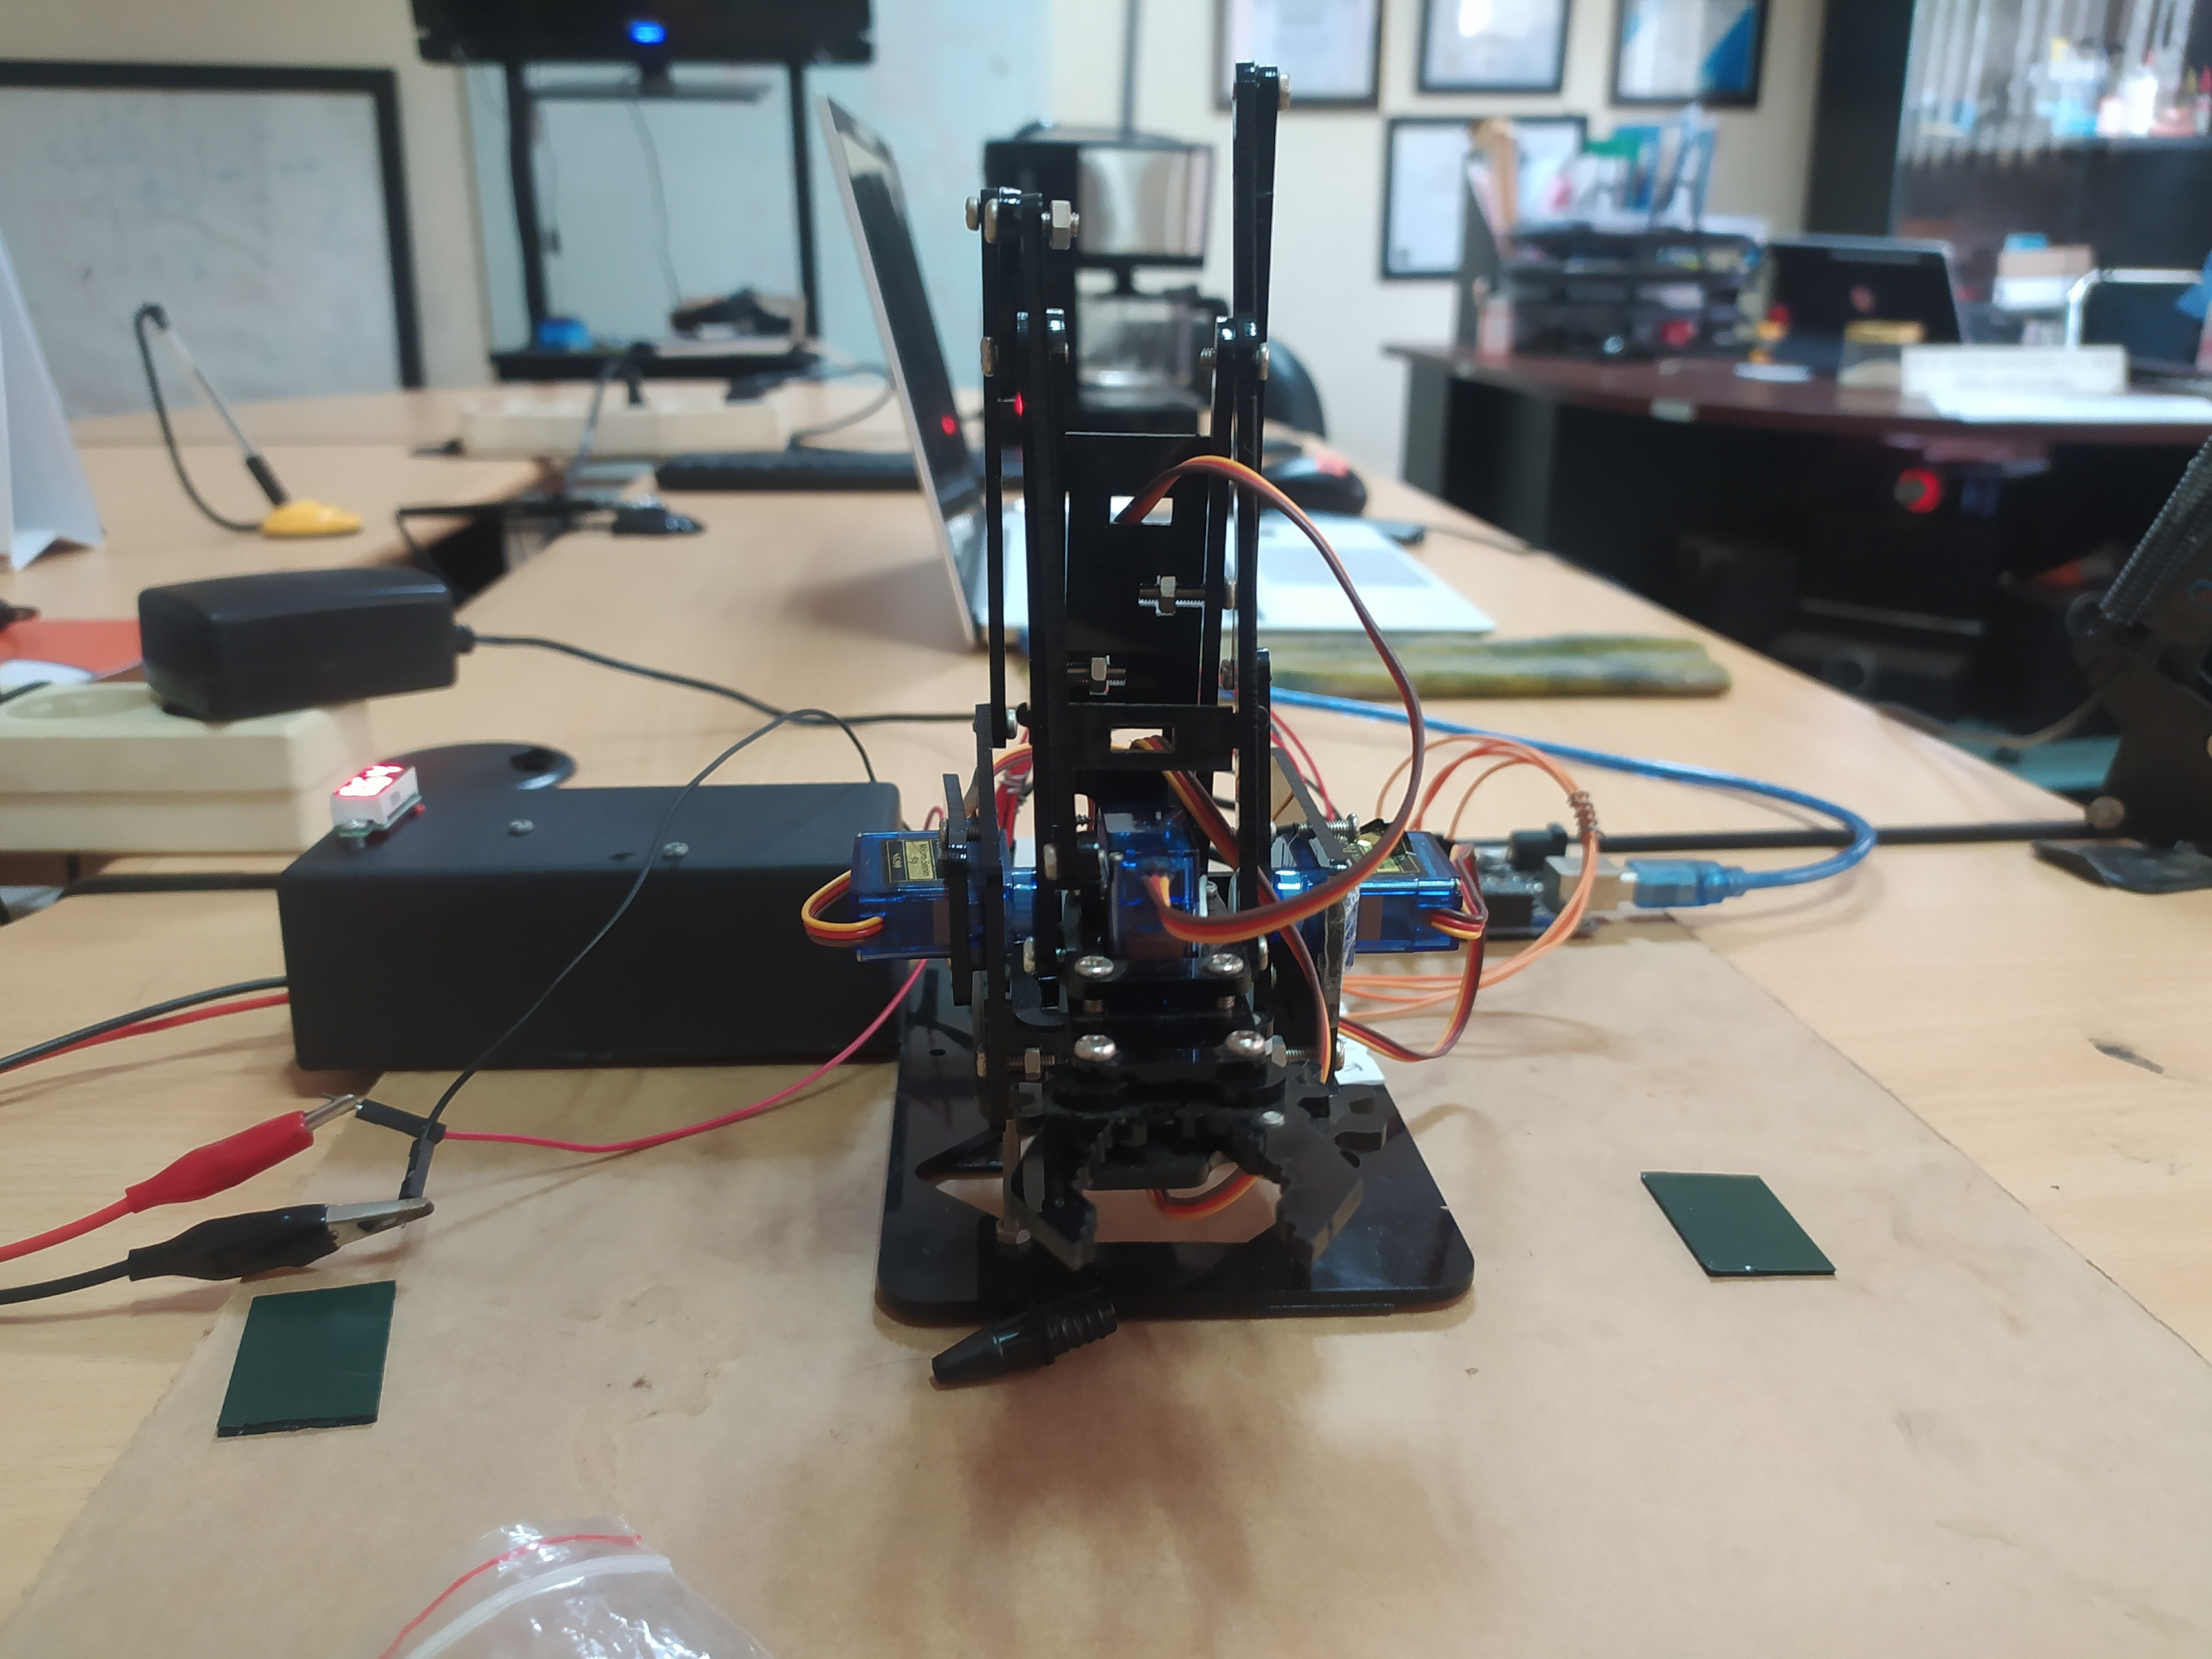
\includegraphics[width=\textwidth]{Gambar/Gambar3_4a_mearm_depan.jpg}
        \caption{Tampak Depan}
        \label{fig:mearm_depan}
    \end{subfigure}
    \hfill
    \begin{subfigure}[b]{0.48\textwidth}
        \centering
        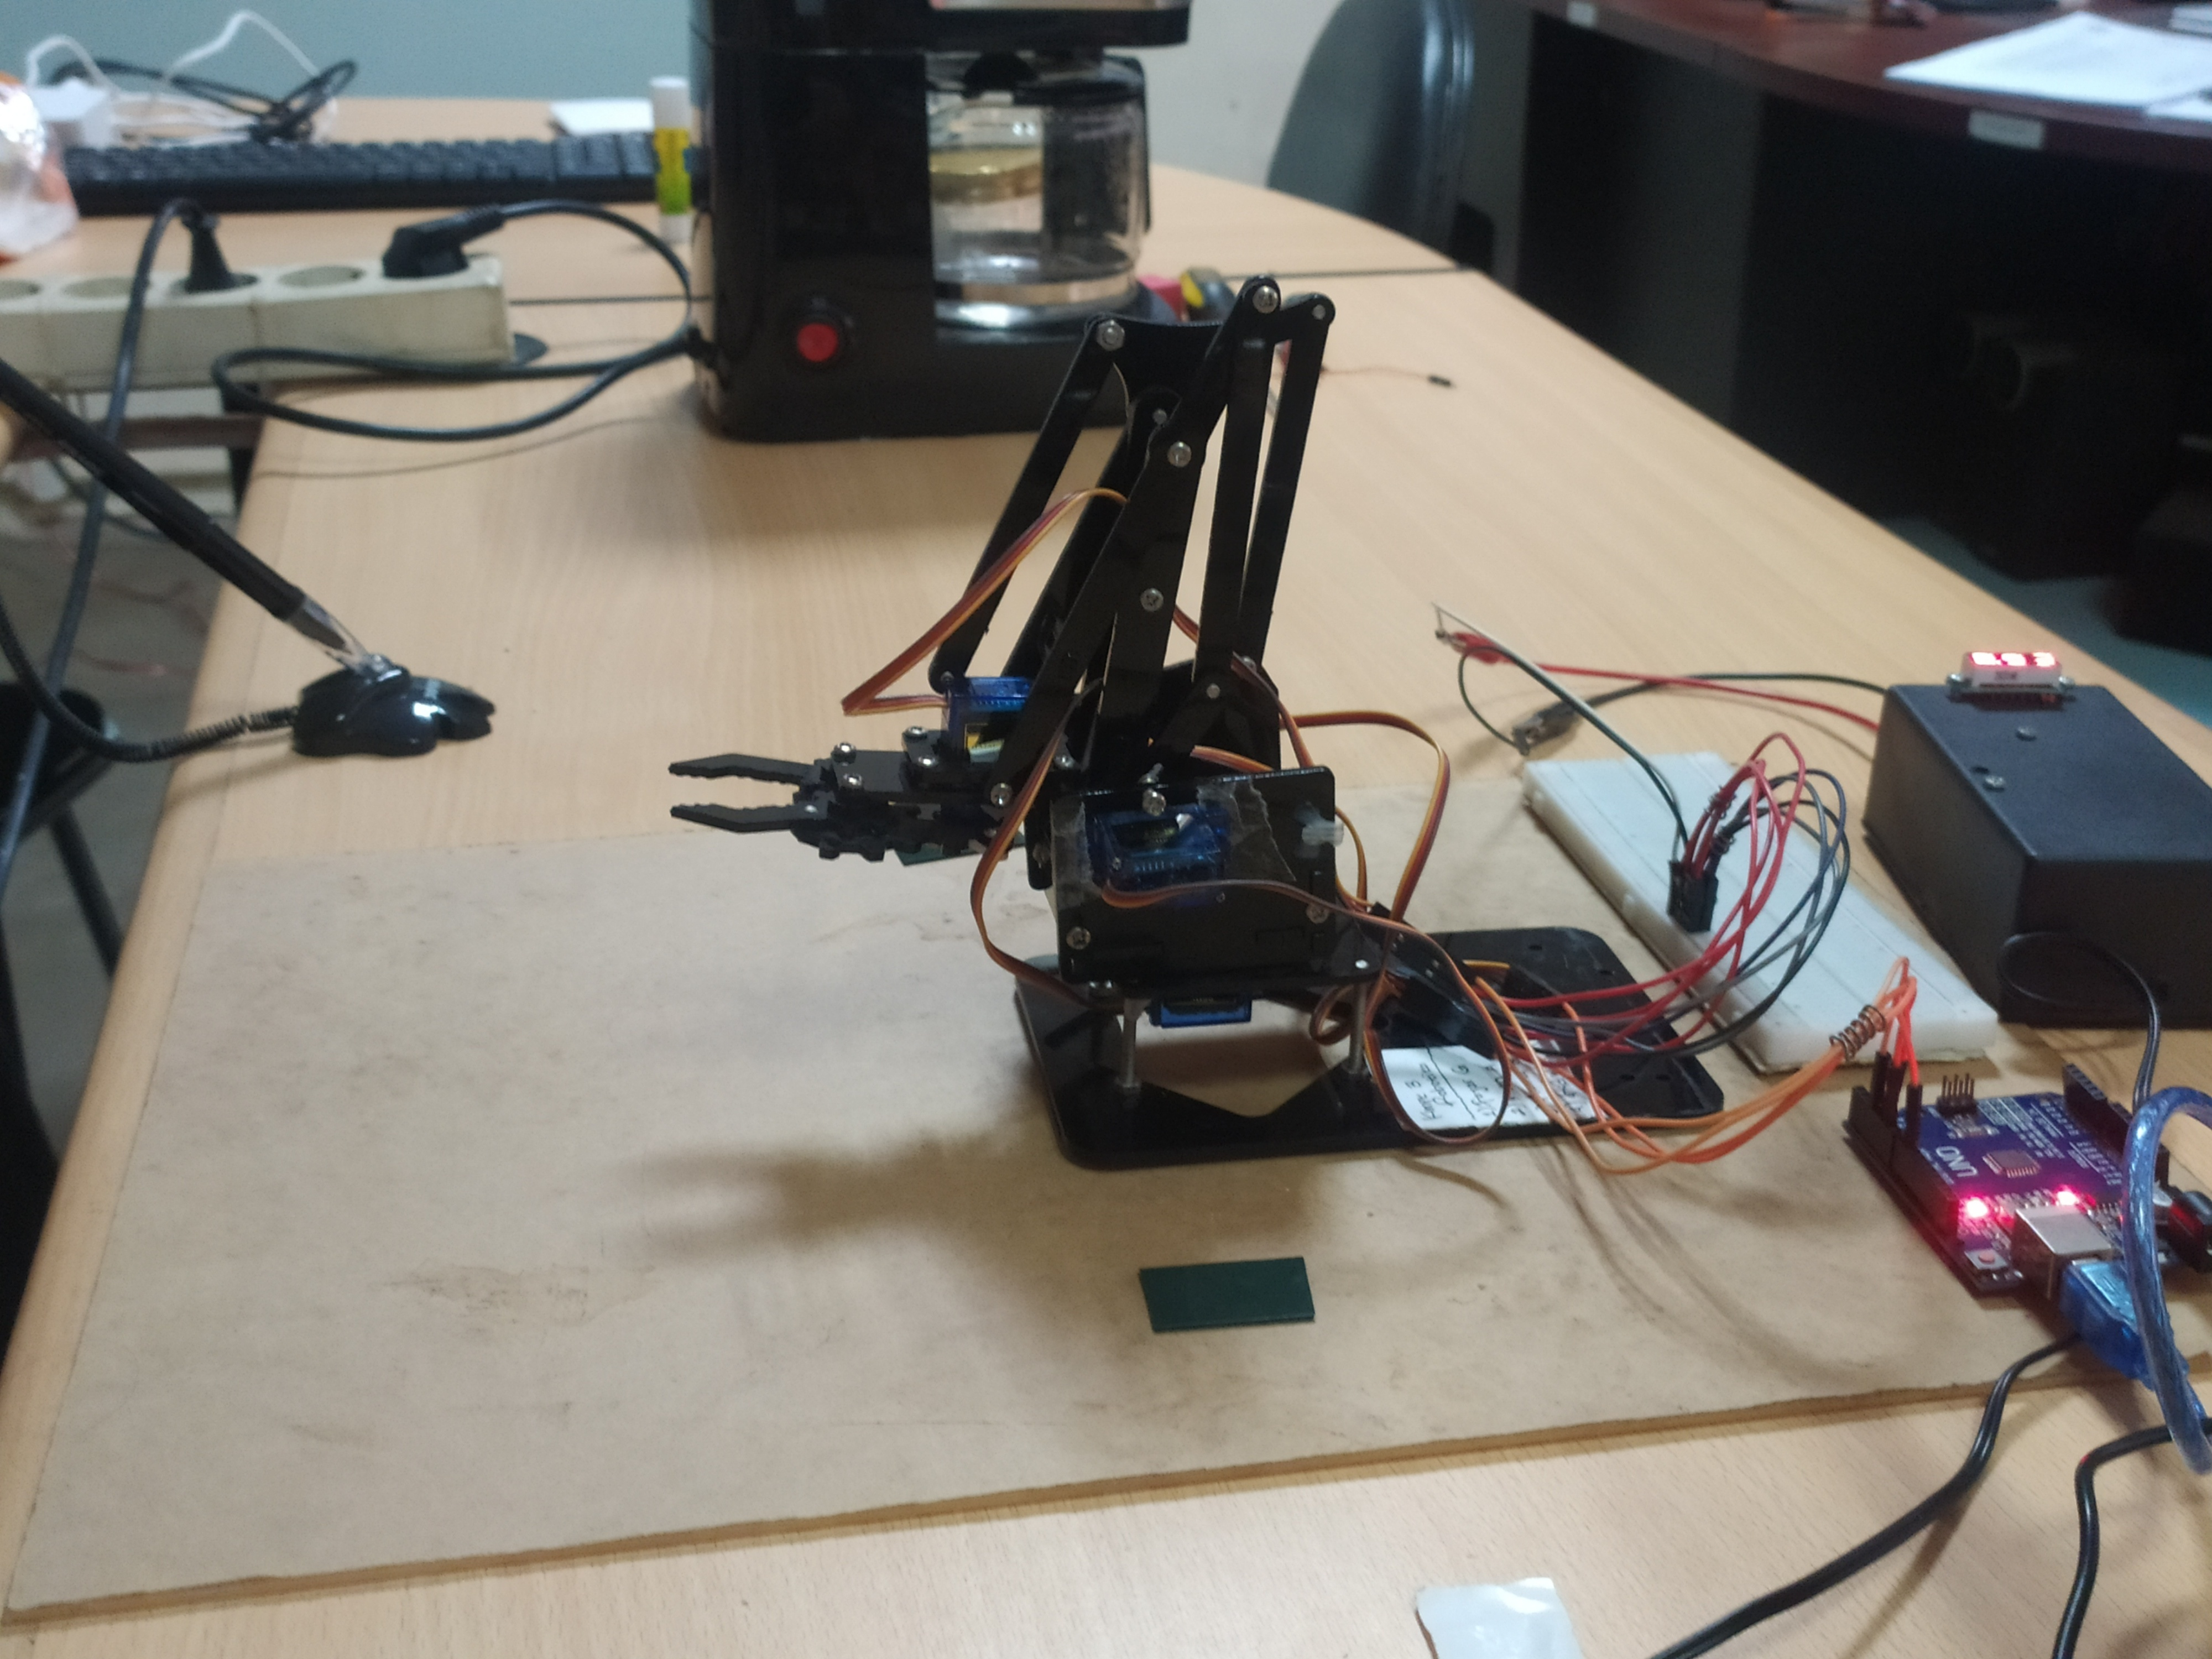
\includegraphics[width=\textwidth]{Gambar/Gambar3_4b_mearm_samping.jpg}
        \caption{Tampak Samping}
        \label{fig:mearm_samping}
    \end{subfigure}
    \caption{Purwarupa Lengan Robot meArm 4-DOF: (a) Tampak Depan dan (b) Tampak Samping untuk Mode Pengenalan SIBI}
    \label{fig:mearm_prototype}
\end{figure}

\section{Python 3.9}
Python 3.9 digunakan sebagai bahasa pemrograman utama karena memiliki sintaks yang ringkas, dukungan pustaka yang luas, serta kompatibilitas dengan banyak modul visi komputer dan komunikasi perangkat keras. Python 3.9 dirilis dengan berbagai penyempurnaan bahasa dan pustaka standar \cite{python39}. Pada penelitian ini, Python digunakan untuk membaca kamera, menjalankan MediaPipe, mengolah \textit{landmark} tangan, melakukan klasifikasi sederhana, mengirim perintah ke robot, serta mencatat data pengujian.

Selain Python, pustaka seperti NumPy dapat digunakan untuk operasi matriks dan pengolahan \textit{array} numerik \cite{harris2020}. Hal ini penting karena pemetaan koordinat, normalisasi fitur, dan perhitungan kinematika membutuhkan operasi vektor dan matriks yang efisien.

\chapter{METODE PENELITIAN}

\section{Waktu dan Tempat Pelaksanaan Penelitian}
Penelitian ini dilaksanakan pada bulan Januari hingga Februari 2026 di Laboratorium Program Studi Teknologi Mekatronika, Politeknik Enjinering Indorama (PEI), Kabupaten Purwakarta, Jawa Barat.

\section{Alat dan Bahan}
Adapun rincian spesifikasi serta kuantitas alat dan bahan yang digunakan pada penelitian ini disajikan pada Tabel \ref{tab:alat_bahan}.

\begin{table}[htbp]
\centering
\caption{Alat dan Bahan}
\label{tab:alat_bahan}
\begin{tabular}{|c|p{8.5cm}|c|}
\hline
\textbf{No.} & \multicolumn{1}{c|}{\textbf{Alat dan Bahan}} & \textbf{Jumlah} \\ \hline
1. & Laptop & 1 buah \\ \hline
2. & Raspberry Pi 5 & 1 buah \\ \hline
3. & Lengan Robot Dobot Magician & 1 buah \\ \hline
4. & Lengan Robot meArm (4-DOF) & 1 buah \\ \hline
5. & Kamera Web (Webcam) Logitech [Model: C270/HD] \newline (Resolusi: 640$\times$480 piksel, 30 FPS) & 1 buah \\ \hline
6. & Monitor Raspberry Pi & 1 buah \\ \hline
7. & Adaptor Daya (\textit{Power Supply}) Raspberry Pi & 1 buah \\ \hline
8. & \textit{Power Supply} 5V DC (untuk meArm) & 1 buah \\ \hline
9. & Papan Rangkaian (\textit{Breadboard}) & 1 buah \\ \hline
10. & Kabel \textit{Jumper} (\textit{Male-to-Male}/\textit{Male-to-Female}) & Secukupnya \\ \hline
11. & Kabel USB Serial & 1 buah \\ \hline
12. & Software Python 3.9 & - \\ \hline
13. & Pustaka Python: OpenCV (v4.9.0.80), MediaPipe (v0.9.0.1), TensorFlow/Keras, NumPy (v1.23.5), Protobuf (v3.20.3), Pydobotplus, PySerial, Tkinter, dan Pillow (PIL) & - \\ \hline
\end{tabular}
\end{table}

\section{Diagram Alir}
Adapun diagram alir penelitian ini adalah sebagai berikut.

\begin{figure}[htbp]
\centering
\begin{tikzpicture}[
    node distance=1.3cm,
    every node/.style={fill=white, font=\small},
    block/.style={rectangle, draw=black, rounded corners, fill=blue!10, text width=7.5cm, text centered, minimum height=1cm, line width=0.8pt},
    arrow/.style={thick, ->, >=stealth}
]
    \node (step1) [block] {Menyiapkan alat dan bahan};
    \node (step2) [block, below of=step1] {Pelaksanaan studi literatur};
    \node (step3) [block, below of=step2] {Perancangan \textit{hardware} sistem kendali lengan robot};
    \node (step4) [block, below of=step3] {Perancangan piranti lunak eksperimen};
    \node (step5) [block, below of=step4] {Penyusunan desain utama rangkaian secara keseluruhan};
    \node (step6) [block, below of=step5] {Pengujian sistem};

    \draw [arrow] (step1) -- (step2);
    \draw [arrow] (step2) -- (step3);
    \draw [arrow] (step3) -- (step4);
    \draw [arrow] (step4) -- (step5);
    \draw [arrow] (step5) -- (step6);
\end{tikzpicture}
\caption{Diagram Alir Penelitian}
\label{fig:diagram_alir}
\end{figure}

Penelitian ini diinisiasi dengan melaksanakan riset terkait studi literatur dari diversifikasi sumber yang teruji validitasnya. Riset ini dilakukan untuk menganalisis secara mendalam terkait landasan teori dari topik yang diteliti, menganalisis prinsip dan langkah kerja dari eksperimen yang dilakukan, dan memahami prinsip kerja dari alat yang digunakan dalam menunjang efektivitas eksperimen. Setelah dilaksanakan riset studi literatur, tahapan selanjutnya adalah perancangan \textit{hardware} dari sistem kendali lengan robot, mencakup di dalamnya pemilihan komponen dan memahami prinsip kerja, \textit{datasheet}, dan alur rangkaian dari purwarupa yang disusun.

Langkah selanjutnya setelah rangkaian berjalan dengan baik, tahapan yang dilakukan adalah menyusun piranti lunak, mencakup di dalamnya kode program terkait ekstraksi \textit{landmark} pengenalan SIBI dan algoritma kinematika, serta program antarmuka menggunakan piranti Python 3.9. Tahapan yang ditempuh setelah rangkaian \textit{hardware} dan tampilan antarmuka berjalan dengan baik dan konsisten, maka tahapan yang dilaksanakan adalah penyusunan desain utama rangkaian secara keseluruhan. Setelah seluruh tahapan dilakukan, maka tahapan akhir yang ditempuh adalah pengujian sistem secara keseluruhan. Tahapan ini mencakup di dalamnya pengukuran data dan pengolahan data serta membandingkan hasil yang diperoleh dengan referensi yang ada untuk memvalidasi efektivitas sistem.

\subsection{Studi Literatur}
Studi literatur yang ditempuh adalah menggunakan referensi yang kredibel, mencakup di dalamnya yaitu referensi berdasarkan jurnal terakreditasi, buku, dan dokumen resmi terkait prinsip kerja dari komponen yang digunakan. Literatur ini mencakup di dalamnya terkait teori yang mendasari ekstraksi \textit{landmark} MediaPipe, prosedur kerja eksperimen yang ditempuh, prinsip kerja dari aktuator lengan robot, prosedur kerja dari persamaan trigonometri \textit{Inverse Kinematics} yang disusun, pemodelan jaringan \textit{Deep Neural Networks} (DNN), dan tahapan pengukuran maupun pengolahan data yang dilakukan.

\subsection{Perancangan \textit{Hardware} Sistem Kendali Robot}
Pada tahap ini, tahapan prosedur difokuskan dalam penyusunan rangkaian secara elektronika. Penyusunan rangkaian dimulai dari penempatan aktuator Dobot Magician dan perakitan mekanis lengan robot meArm, yang keduanya diintegrasikan dengan modul Raspberry Pi 5 sebagai \textit{edge computer} utama yang terhubung ke Monitor Raspberry Pi. Kemudian, penyusunan rangkaian turut dilaksanakan dengan menghubungkan beberapa pin utama yang menghubungkan aktuator servo meArm terhadap pin GPIO mikrokontroler melalui bantuan \textit{breadboard} dan kabel \textit{jumper}.

Adaptor daya kustom dialokasikan khusus untuk menyuplai daya komputasi Raspberry Pi 5 agar tidak mengalami \textit{under-voltage}, sedangkan \textit{power supply} 5V DC eksternal digunakan untuk menyuplai arus penggerak motor servo meArm secara terpisah agar sistem terhindar dari gangguan \textit{noise} induksi motor. Kabel USB Serial juga dipasangkan secara fisik untuk menjamin kestabilan transmisi instruksi sudut dan koordinat dari port USB Raspberry Pi 5 menuju \textit{internal controller} Dobot Magician.

\subsection{Perancangan Piranti Lunak}
Tahapan perancangan piranti lunak mencakup penyusunan arsitektur pemrograman berbasis Python 3.9 yang mengintegrasikan pemrosesan citra, ekstraksi fitur penanda geometris, klasifikasi kecerdasan buatan, manajemen antarmuka grafis (\textit{Graphical User Interface}), dan komunikasi serial. Secara teknis, fungsionalitas piranti lunak ini dirancang menggunakan kontribusi dari beberapa pustaka utama dengan mekanisme kerja sebagai berikut:

Dalam inisialisasi awal program, sistem meluncurkan antarmuka pengguna grafis (GUI) yang dibangun menggunakan pustaka Tkinter. GUI ini memfasilitasi interaksi pengguna untuk memantau konektivitas robot, mengelola \textit{jogging} secara manual, serta memvisualisasikan mode kendali berbasis AI. Sementara itu, pustaka OpenCV (v4.9.0.80) dikonfigurasi untuk membuka saluran komunikasi visual dengan \textit{webcam} Logitech. OpenCV bertugas melakukan akuisisi bingkai (\textit{frame}) video secara \textit{real-time}, membalikkan citra secara horizontal (\textit{mirroring}), serta melakukan konversi ruang warna dari BGR ke RGB. Agar aliran citra visual tersebut dapat dirender dan ditanamkan (\textit{embedded}) ke dalam kanvas antarmuka Tkinter, program memanfaatkan pustaka Pillow (PIL) untuk mengonversi matriks array NumPy menjadi objek gambar (ImageTk) yang kompatibel dengan komponen GUI.

Setelah citra RGB diperoleh, data diumpankan secara langsung ke dalam kerangka kerja MediaPipe (v0.9.0.1). Di dalam struktur perulangan (\textit{main loop}), MediaPipe mengeksekusi model deteksi untuk mengekstrak 21 titik persendian spasial (\textit{landmarks}) dalam koordinat tiga dimensi $(x,y,z)$. Koordinat ini kemudian didistribusikan ke dalam dua logika kondisional berdasarkan mode operasi robot:

\begin{enumerate}[label=\arabic*.]
    \item \textbf{Alur Kerja Mode SIBI (meArm)}: Matriks koordinat 21 persendian tangan ditransformasikan ke dalam larik 1D dan dinormalisasi terhadap titik pergelangan (\textit{wrist}). Vektor fitur spasial yang telah siap kemudian diumpankan maju (\textit{feed-forward}) ke dalam model \textit{Deep Neural Networks} (DNN) yang dimuat menggunakan pustaka TensorFlow/Keras. Kestabilan struktur \textit{array} dan komputasi matriks pada tahap ini dijaga sepenuhnya oleh pustaka NumPy (v1.23.5), sementara kompatibilitas pemuatan arsitektur model diregulasi oleh pustaka Protobuf (v3.20.3). Jika nilai probabilitas klasifikasi abjad melampaui batas ambang batas (\textit{confidence score} $> 0.8$), perintah dipetakan menjadi koordinat tujuan (\textit{waypoint}) yang kemudian dikirim via serial komunikasi untuk menggerakkan meArm.
    \item \textbf{Alur Kerja Mode Teleoperasi (Dobot Magician)}: Program memetakan koordinat titik \textit{wrist} dan \textit{index finger tip}, lalu mengonversinya menjadi koordinat kerja spasial absolut robot $(X,Y,Z)$ melalui algoritma \textit{Inverse Kinematics} berbasis komputasi NumPy. Untuk mentransmisikan matriks target secara instan, program ditunjang oleh pustaka PySerial di tingkat \textit{low-level} serta pustaka Pydobotplus di tingkat operasional. Keunggulan kolaborasi kedua pustaka komunikasi ini berhasil mengeliminasi \textit{bug packet loss} dan menstabilkan \textit{buffer} instruksi \textit{Point-to-Point} (PTP), sehingga lengan robot Dobot Magician bergerak mulus meniru gestur operator tanpa adanya getaran (\textit{jitter}).
\end{enumerate}

\subsection{Pengujian}
Pada tahapan akhir, pengujian sistem dilaksanakan pada alat yang telah disusun, kemudian menghitung dan membandingkan data akurasi serta latensi yang diperoleh terhadap parameter respons target untuk memvalidasi keakuratan dan ketelitian data yang diperoleh. Pengujian alat ini dilakukan dengan memberikan input formasi jari langsung di hadapan \textit{webcam} Logitech untuk memperoleh beragam kelas dataset gestur abjad. Kemudian, sensor kamera akan mencatat nilai koordinat persendian secara kontinu dan mengkalkulasi prediksi secara otomatis. Data yang diperoleh kemudian akan ditampilkan secara visual pada antarmuka GUI Tkinter berupa label abjad SIBI yang diklasifikasikan beserta matriks koordinat Cartesian yang tengah dieksekusi oleh mesin robot.

\chapter{HASIL DAN PEMBAHASAN}

\section{Hasil Perancangan Sistem Tertanam}
Hasil perancangan sistem tertanam berupa arsitektur kendali berbasis Raspberry Pi 5 yang menghubungkan kamera, \textit{pipeline} MediaPipe, modul pemilihan mode, dan dua robot manipulator. Sistem dibagi menjadi dua mode utama, yaitu mode pengenalan SIBI pada meArm dan mode teleoperasi pada Dobot Magician. Pembagian mode ini bertujuan agar satu perangkat komputasi dapat menjalankan dua fungsi interaksi manusia--robot yang berbeda.

Secara umum, alur sistem dimulai dari akuisisi citra tangan oleh kamera. Citra tersebut diproses oleh MediaPipe untuk menghasilkan \textit{landmark} tangan. \textit{Landmark} kemudian dikirim ke modul pengolah fitur. Jika sistem berada pada mode SIBI, fitur digunakan untuk klasifikasi isyarat. Jika sistem berada pada mode teleoperasi, fitur digunakan untuk menentukan koordinat target robot. Hasil rancangan arsitektur sistem ditunjukkan pada Gambar \ref{fig:arsitektur_sistem}.

\begin{figure}[htbp]
\centering
\begin{tikzpicture}[
    node distance=1.5cm,
    font=\small,
    box/.style={rectangle, draw=black, rounded corners, fill=blue!10, text centered, minimum height=0.9cm, text width=3.2cm, line width=0.8pt},
    decision/.style={diamond, draw=black, fill=orange!20, text centered, inner sep=2pt, line width=0.8pt},
    arrow/.style={thick, ->, >=stealth}
]
    % Container box for RPi 5
    \draw[dashed, fill=gray!5, line width=0.8pt] (-4.5, -4.5) rectangle (7.5, 1.8);
    \node at (1.5, 1.4) [font=\bfseries] {Raspberry Pi 5 (Edge Computer)};

    % Top nodes
    \node (cam) [box, text width=2.6cm] at (-3, 0.4) {Kamera Web\\Logitech};
    \node (mp) [box, text width=2.8cm] at (0.2, 0.4) {MediaPipe\\Hands};
    \node (ext) [box, text width=3.2cm] at (4.0, 0.4) {Ekstraksi 21\\Landmark $(x,y,z)$};

    % Decision node
    \node (dec) [decision] at (4.0, -1.5) {Mode?};

    % Branch 1: SIBI
    \node (dnn) [box, text width=2.8cm] at (1.2, -2.6) {DNN Klasifikasi\\SIBI};
    \node (mearm) [box, text width=2.8cm, fill=green!15] at (-2.5, -2.6) {meArm 4-DOF\\(Serial)};

    % Branch 2: Teleoperation
    \node (ik) [box, text width=3.0cm] at (4.0, -3.8) {Pemetaan IK\\Koordinat Spasial};
    \node (dobot) [box, text width=2.8cm, fill=green!15] at (-0.5, -3.8) {Dobot Magician\\(USB)};

    % Connections
    \draw [arrow] (cam) -- (mp);
    \draw [arrow] (mp) -- (ext);
    \draw [arrow] (ext) -- (dec);
    \draw [arrow] (dec) -| node[above, font=\footnotesize, xshift=1cm] {SIBI} (dnn);
    \draw [arrow] (dnn) -- (mearm);
    \draw [arrow] (dec) -- node[right, font=\footnotesize] {Teleoperasi} (ik);
    \draw [arrow] (ik) -- (dobot);
\end{tikzpicture}
\caption{Hasil Rancangan Arsitektur Sistem Tertanam Berbasis Raspberry Pi 5}
\label{fig:arsitektur_sistem}
\end{figure}

Pembahasan pada tahap ini perlu menekankan bahwa Raspberry Pi 5 tidak hanya berfungsi sebagai pengendali aktuator, tetapi juga sebagai simpul komputasi tepi. Dengan demikian, pengolahan citra, ekstraksi \textit{landmark}, pengambilan keputusan, dan pengiriman perintah dapat dilakukan secara lokal. Hal ini mendukung pengurangan latensi dan membuat sistem lebih portabel dibanding rancangan yang bergantung pada komputer eksternal atau \textit{server}.

\section{Pengujian Mode Pengenalan SIBI pada meArm}
Mode pengenalan SIBI diuji dengan memberikan sejumlah isyarat tangan ke kamera, kemudian sistem mengklasifikasikan isyarat tersebut menjadi label perintah. Label yang dikenali selanjutnya dipetakan ke gerakan meArm. Contoh pemetaan perintah dapat dilihat pada Tabel \ref{tab:pemetaan_sibi}. Tabel ini dapat disesuaikan dengan kelas SIBI yang digunakan saat pengambilan data.

\begin{table}[htbp]
\centering
\caption{Pemetaan Isyarat Abjad SIBI terhadap Respons Kendali meArm}
\label{tab:pemetaan_sibi}
\begin{tabular}{|c|c|p{4.5cm}|p{5.5cm}|}
\hline
\textbf{No.} & \textbf{Karakter} & \multicolumn{1}{c|}{\textbf{Klasifikasi Isyarat}} & \multicolumn{1}{c|}{\textbf{Respons Kinematika meArm}} \\ \hline
1 & 'A' & Kepalan ibu jari ke atas & Bergerak maju ke target posisi $XYZ(80, 0, 40)$ mm \\ \hline
2 & 'B' & Empat jari tegak rapat & Bergerak rotasi ke posisi kerja $XYZ(60, 60, 30)$ mm \\ \hline
3 & 'C' & Jari melengkung kurva & Menutup capit \textit{gripper} (sudut servo $90^\circ$) \\ \hline
4 & 'D' & Telunjuk tegak vertikal & Membuka capit \textit{gripper} (sudut servo $180^\circ$) \\ \hline
5 & 'E' & Empat jari menekuk & Kembali ke posisi parkir awal (\textit{home}) \\ \hline
\end{tabular}
\end{table}

Berdasarkan skema pemetaan pada Tabel \ref{tab:pemetaan_sibi}, pergerakan translasi posisi lengan robot meArm maupun kendali capit (\textit{gripper}) diatur secara terarah terhadap hasil klasifikasi isyarat tangan.

\subsection{Akurasi Klasifikasi Isyarat SIBI}
Sebelum model diimplementasikan ke dalam kendali aktuator meArm, dilakukan pelatihan model \textit{Deep Neural Network} (DNN) menggunakan arsitektur \textit{fully-connected} dengan pengoptimal Adam dan fungsi kerugian \textit{categorical cross-entropy}. Proses pelatihan model ini dilaksanakan pada tahap magang Minggu ke-3, tepatnya tanggal 25 Januari 2026. Dinamika proses pelatihan model dievaluasi melalui grafik akurasi terhadap \textit{epoch} dan grafik \textit{loss} terhadap \textit{epoch} yang disajikan berdampingan pada Gambar \ref{fig:evaluasi_dnn}.

\begin{figure}[htbp]
    \centering
    \begin{subfigure}[b]{0.48\textwidth}
        \centering
        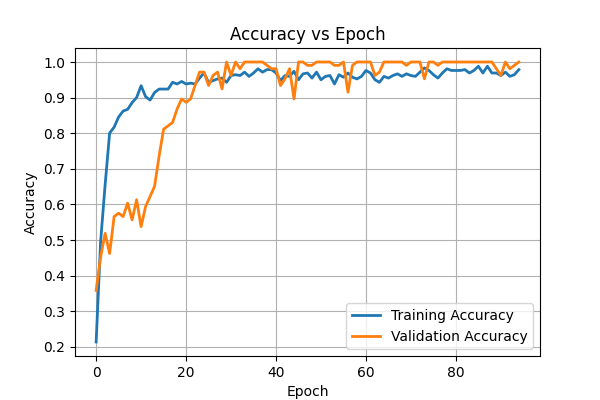
\includegraphics[width=\textwidth]{Gambar/Gambar5_2a_akurasi_sibi.png}
        \caption{Akurasi vs Epoch}
        \label{fig:akurasi_epoch}
    \end{subfigure}
    \hfill
    \begin{subfigure}[b]{0.48\textwidth}
        \centering
        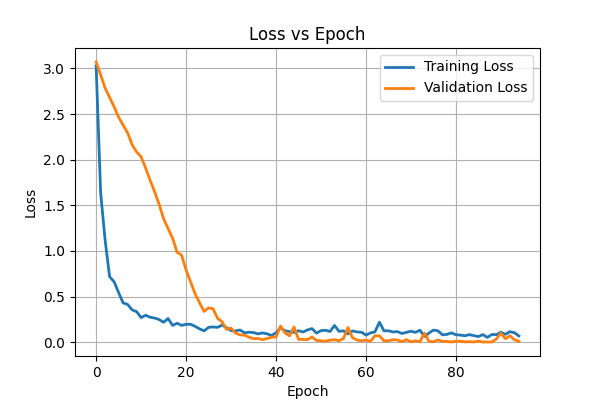
\includegraphics[width=\textwidth]{Gambar/Gambar5_2b_loss_sibi.png}
        \caption{Loss vs Epoch}
        \label{fig:loss_epoch}
    \end{subfigure}
    \caption{Kurva Evaluasi Pelatihan Model DNN SIBI (Sesi Pelatihan 25 Januari 2026): (a) \textit{Accuracy vs Epoch}, (b) \textit{Loss vs Epoch}}
    \label{fig:evaluasi_dnn}
\end{figure}

Berdasarkan Gambar \ref{fig:evaluasi_dnn}, pada kurva akurasi (sisi kiri), nilai akurasi data latih (\textit{Training Accuracy}) meningkat secara pesat pada 20 \textit{epoch} pertama dari 21,3\% hingga melampaui 90,0\%, dan mencapai kestabilan pada rentang 96,0\% hingga 98,5\%. Akurasi validasi (\textit{Validation Accuracy}) turut menunjukkan kenaikan yang konsisten hingga mencapai 98,0\%--100,0\%. Pada kurva \textit{loss} (sisi kanan), nilai \textit{Training Loss} dan \textit{Validation Loss} mengalami peluruhan eksponensial yang tajam dari nilai awal sekitar 3,08 hingga menyusut di bawah 0,10. Nilai kerugian validasi yang terus berimpit rendah dengan nilai kerugian latih mengonfirmasi bahwa proses optimasi konvergen dengan sangat baik serta model terbebas dari kendala \textit{overfitting}.

Kinerja klasifikasi pada data uji dihitung dengan membandingkan jumlah prediksi benar terhadap seluruh data uji menggunakan persamaan:
\begin{equation}
\text{Akurasi} = \frac{\text{Jumlah prediksi benar}}{\text{Jumlah seluruh data uji}} \times 100\%.
\label{eq:akurasi}
\end{equation}

Evaluasi keandalan pengenalan isyarat SIBI selanjutnya dianalisis melalui dua tahapan pengujian yang selaras dengan linimasa eksperimen magang:
\begin{enumerate}[label=\arabic*.]
    \item \textbf{Pengujian Data Validasi Latih (25 Januari 2026)}: Evaluasi dilakukan langsung pasca-pelatihan model terhadap 106 sampel data uji validasi (sekitar 4--6 data per kelas huruf). Sebagaimana ditunjukkan pada Gambar \ref{fig:cm_validasi}, seluruh elemen prediksi terkonsentrasi penuh pada diagonal utama matriks dari huruf A hingga Z tanpa adanya kesalahan prediksi silang (\textit{off-diagonal} bernilai 0). Hal ini membuktikan bahwa pembobotan fitur 63 koordinat spasial telah terpetakan sempurna pada data uji latih.
    \item \textbf{Pengujian Sistem Secara \textit{Real-Time} (18 Februari 2026)}: Untuk menguji keandalan sistem dalam kondisi operasional nyata, pengujian eksperimental dilakukan pada akhir masa magang di hadapan kamera secara langsung dengan Raspberry Pi 5. Pada pengujian ini, setiap abjad diuji sebanyak 20 kali percobaan (total 520 data uji). Distribusi hasil pengujian nyata disajikan pada Gambar \ref{fig:cm_realtime}.
\end{enumerate}

\begin{figure}[htbp]
    \centering
    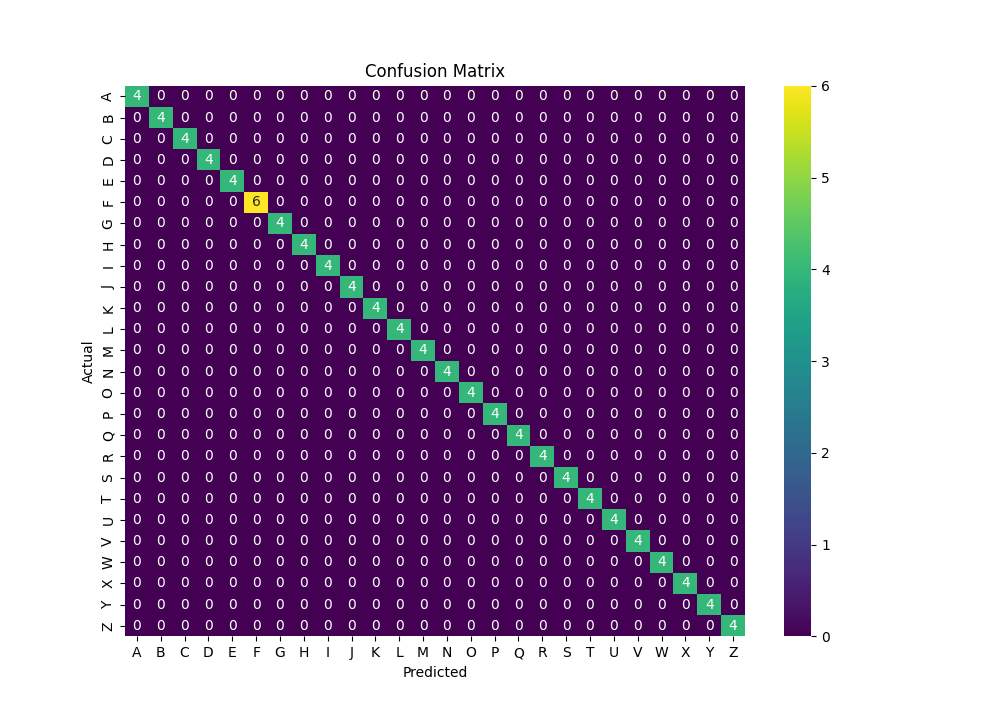
\includegraphics[width=0.82\textwidth]{Gambar/Gambar5_3_cm_validasi.png}
    \caption{Matriks Kebingungan Pengujian Validasi Awal Model SIBI (Sesi 25 Januari 2026)}
    \label{fig:cm_validasi}
\end{figure}

\begin{figure}[htbp]
    \centering
    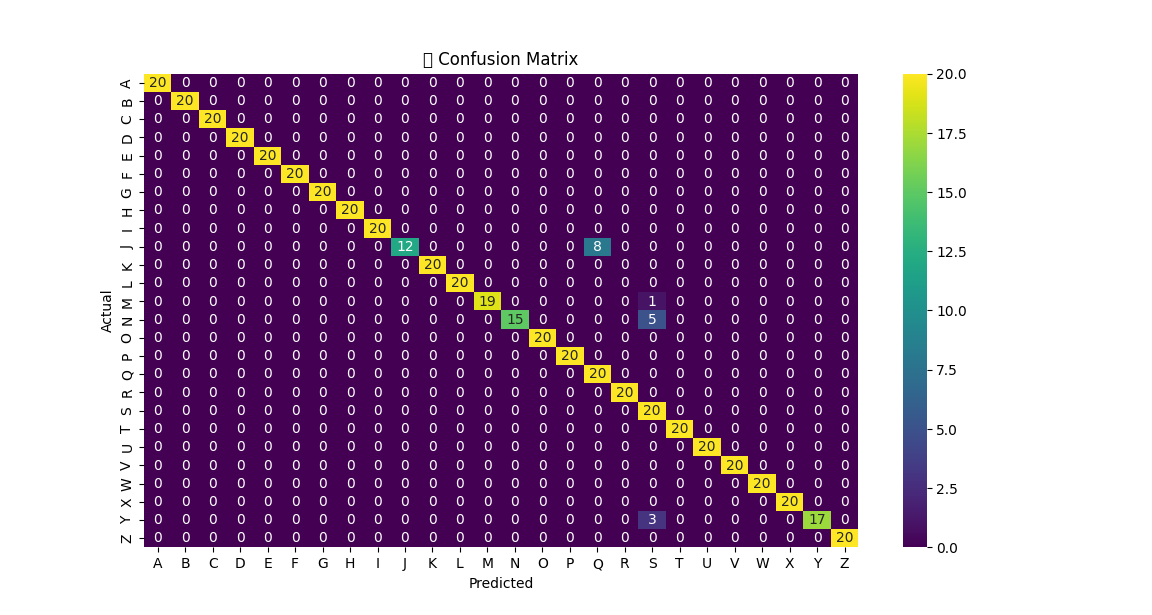
\includegraphics[width=0.88\textwidth]{Gambar/Gambar5_4_cm_realtime.png}
    \caption{Matriks Kebingungan Pengujian Sistem \textit{Real-Time} SIBI dengan 20 Data Uji per Abjad (Sesi 18 Februari 2026)}
    \label{fig:cm_realtime}
\end{figure}

Berdasarkan hasil pengujian nyata pada Gambar \ref{fig:cm_realtime}, dari total 520 kali pengujian isyarat, sistem berhasil memprediksi 503 data dengan tepat, menghasilkan akurasi sistem secara keseluruhan sebesar \textbf{96,73\%}. Sebanyak 22 kelas alfabet berhasil dikenali dengan akurasi 100,0\% (20 dari 20 percobaan). Rekapitulasi hasil pengujian per kelompok isyarat disajikan pada Tabel \ref{tab:rekap_sibi}.

\begin{table}[htbp]
\centering
\caption{Rekapitulasi Kinerja Pengujian Sistem SIBI (Sesi 18 Februari 2026)}
\label{tab:rekap_sibi}
\begin{tabular}{|c|p{6cm}|c|c|c|}
\hline
\textbf{No.} & \multicolumn{1}{c|}{\textbf{Kelompok Isyarat}} & \textbf{Data Uji} & \textbf{Prediksi Benar} & \textbf{Akurasi (\%)} \\ \hline
1 & Isyarat Perintah Utama (A--E) & 100 & 100 & 100,0 \\ \hline
2 & Isyarat Sekunder (F--J) & 100 & 92 & 92,0 \\ \hline
3 & Isyarat Lanjutan 1 (K--R) & 160 & 154 & 96,25 \\ \hline
4 & Isyarat Lanjutan 2 (S--Z) & 160 & 157 & 98,13 \\ \hline
\multicolumn{2}{|c|}{\textbf{Total Kinerja Keseluruhan (520 Pengujian)}} & \textbf{520} & \textbf{503} & \textbf{96,73} \\ \hline
\end{tabular}
\end{table}

Berdasarkan data pada Tabel \ref{tab:rekap_sibi}, kelompok isyarat perintah utama (A--E) yang menjadi dasar kendali aktuator robot meArm berhasil mencapai akurasi sempurna sebesar 100,0\%. Tingginya akurasi klasifikasi ini didukung oleh penggunaan 63 fitur koordinat spasial ternormalisasi dari 21 titik persendian \textit{MediaPipe Hand Landmarks}. Normalisasi koordinat terhadap titik pergelangan tangan (\textit{wrist}) berhasil mengeliminasi variasi posisi tangan relatif terhadap sudut pandang kamera, sehingga model DNN dapat membedakan formasi kelengkungan jari secara tegas dan konsisten.

\subsection{Analisis Pergerakan Kinematis meArm}
Analisis pergerakan kinematis meArm dilakukan dengan mengamati respons servo terhadap hasil klasifikasi. Hasil pengujian respons fisik motor servo meArm terhadap kelima isyarat SIBI yang berhasil diklasifikasikan disajikan pada Tabel \ref{tab:respons_mearm}.

\begin{table}[htbp]
\centering
\caption{Pengujian Respons Kinematik meArm terhadap Perintah SIBI}
\label{tab:respons_mearm}
\begin{tabular}{|c|c|p{4cm}|p{5cm}|c|}
\hline
\textbf{No.} & \textbf{Isyarat} & \multicolumn{1}{c|}{\textbf{Perintah Aksi}} & \multicolumn{1}{c|}{\textbf{Respons Fisik Aktual}} & \textbf{Status} \\ \hline
1 & 'A' & Maju ke posisi kerja & Lengan bergerak maju menuju $XYZ(80,0,40)$ mm & Berhasil \\ \hline
2 & 'B' & Rotasi ke posisi samping & Basis berputar ke koordinat $XYZ(60,60,30)$ mm & Berhasil \\ \hline
3 & 'C' & Menutup \textit{gripper} & Capit menutup rapat menjepit silinder uji & Berhasil \\ \hline
4 & 'D' & Membuka \textit{gripper} & Capit membuka penuh melepas silinder & Berhasil \\ \hline
5 & 'E' & Kembali ke posisi \textit{home} & Seluruh servo kembali ke posisi parkir awal & Berhasil \\ \hline
\end{tabular}
\end{table}

Berdasarkan Tabel \ref{tab:respons_mearm}, seluruh lima perintah utama SIBI berhasil diterjemahkan menjadi respons gerak servo meArm secara konsisten. Pergerakan servo berjalan halus tanpa lonjakan mendadak berkat implementasi jeda bertahap (\textit{smooth stepping}) pada firmware. Keterbatasan utama yang diamati adalah rentang kerja fisik meArm yang relatif sempit ($\le 180$ mm jangkauan diagonal), sehingga target koordinat harus dibatasi agar tidak melampaui batas mekanis tautan lengan.

Dokumentasi visual proses pengujian interaksi langsung lengan robot meArm ditunjukkan pada Gambar \ref{fig:uji_mearm}. Pada pengujian tersebut, operator memperagakan isyarat tangan di hadapan kamera komputer jinjing yang menjalankan sistem deteksi penanda tangan (\textit{hand landmarks}) MediaPipe. Ketika gestur terdeteksi secara valid, kontroler memetakan instruksi dan menggerakkan aktuator motor servo meArm untuk bermanuver dan menjepit objek silinder uji di atas meja eksperimen.

\begin{figure}[htbp]
    \centering
    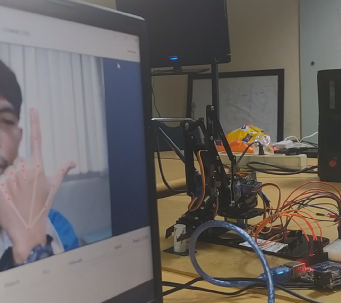
\includegraphics[width=0.85\textwidth]{Gambar/Gambar5_5_uji_mearm_sibi.png}
    \caption{Dokumentasi Pengujian Mode Respons Kinematik meArm Berbasis Deteksi Gestur Tangan}
    \label{fig:uji_mearm}
\end{figure}

\section{Pengujian Mode Teleoperasi pada Dobot Magician}
Mode teleoperasi pada Dobot Magician diuji dengan memetakan gerak tangan pengguna ke posisi target robot. \textit{Landmark} tangan yang dipilih sebagai acuan dapat berupa pergelangan tangan, ujung telunjuk, atau titik tengah telapak. Koordinat citra kemudian dinormalisasi dan diskalakan ke ruang kerja Dobot Magician.

\subsection{Kinerja Pemetaan Koordinat Hand Tracking MediaPipe}
Kinerja pemetaan koordinat dievaluasi dengan membandingkan arah gerak tangan terhadap arah gerak robot. Jika tangan bergerak ke kanan pada citra, robot seharusnya bergerak ke arah yang sesuai pada ruang kerja yang telah didefinisikan. Kalibrasi perlu memperhatikan orientasi kamera karena posisi kamera yang terbalik atau miring dapat menyebabkan arah gerak robot tidak sesuai. Hasil evaluasi pemetaan arah gerak spasial tangan terhadap respons Dobot Magician disajikan pada Tabel \ref{tab:pemetaan_dobot}.

\begin{table}[htbp]
\centering
\caption{Evaluasi Pemetaan Koordinat Hand Tracking ke Dobot Magician}
\label{tab:pemetaan_dobot}
\begin{tabular}{|c|p{4.5cm}|p{5cm}|c|}
\hline
\textbf{No.} & \multicolumn{1}{c|}{\textbf{Arah Gerak Tangan}} & \multicolumn{1}{c|}{\textbf{Respons Dobot Magician}} & \textbf{Kesesuaian Arah} \\ \hline
1 & Geser Kanan ($X > 0{,}5$) & Translasi sumbu $Y+$ (kanan) & Sesuai (Valid) \\ \hline
2 & Geser Kiri ($X < 0{,}5$) & Translasi sumbu $Y-$ (kiri) & Sesuai (Valid) \\ \hline
3 & Angkat Tangan ($Y < 0{,}5$) & Translasi sumbu $Z+$ (naik) & Sesuai (Valid) \\ \hline
4 & Turun Tangan ($Y > 0{,}5$) & Translasi sumbu $Z-$ (turun) & Sesuai (Valid) \\ \hline
5 & Mendekati Kamera ($\text{Skala} > 0{,}2$) & Jangkauan sumbu $X+$ (maju) & Sesuai (Valid) \\ \hline
6 & Jepit Telunjuk--Ibu Jari ($< 30$ px) & Aktivasi Penyedot (\textit{Suction ON}) & Sesuai (Valid) \\ \hline
\end{tabular}
\end{table}

Berdasarkan data pada Tabel \ref{tab:pemetaan_dobot}, seluruh enam aksi arah pergerakan tangan dan gestur operator berhasil dipetakan secara valid dan presisi ke pergerakan fisik Dobot Magician. Pembahasan kinerja pemetaan menunjukkan bahwa penerapan filter \textit{exponential smoothing} ($\alpha = 0{,}2$) dan batas toleransi perubahan jarak gerak (\textit{movement threshold} sebesar 5,0 mm) pada algoritma teleoperasi berhasil mengeliminasi getaran mikro (\textit{jitter}) pada motor penggerak tanpa mengorbankan kelincahan manuver lengan robot.

Pelaksanaan pengujian mode teleoperasi Dobot Magician secara \textit{real-time} ditunjukkan pada Gambar \ref{fig:uji_dobot}. Pada layar komputer jinjing tampak antarmuka pelacakan tangan operator dengan keterangan status ``TANGAN KANAN (On)'' beserta visualisasi graf 21 persendian tangan berbasis MediaPipe. Posisi spasial tangan operator dipetakan secara simultan ke koordinat kerja manipulator Dobot Magician, di mana efektor akhir (\textit{end-effector}) robot yang dilengkapi penyedot vakum (\textit{suction cup}) berhasil dikendalikan secara presisi untuk mengambil dan memindahkan balok kubus objek uji.

\begin{figure}[htbp]
    \centering
    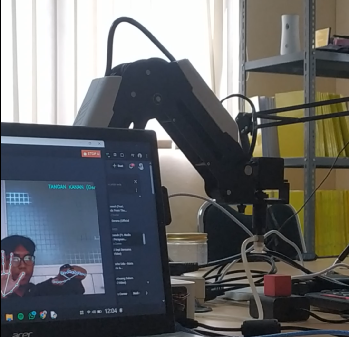
\includegraphics[width=0.85\textwidth]{Gambar/Gambar5_6_uji_teleoperasi_dobot.png}
    \caption{Dokumentasi Pengujian Mode Teleoperasi Dobot Magician Menggunakan Pelacakan Tangan MediaPipe}
    \label{fig:uji_dobot}
\end{figure}

\subsection{Analisis Presisi Spasial dan Waktu Respons Dobot Magician}
Presisi spasial dianalisis dengan membandingkan koordinat target hasil kalkulasi pemetaan algoritma terhadap koordinat aktual yang terbaca dari umpan balik enkoder internal Dobot Magician. Selisih posisi dihitung menggunakan galat Euclidean 3D:
\begin{equation}
e = \sqrt{(X_{\text{target}} - X_{\text{aktual}})^2 + (Y_{\text{target}} - Y_{\text{aktual}})^2 + (Z_{\text{target}} - Z_{\text{aktual}})^2}.
\label{eq:galat_euclidean}
\end{equation}

Pengujian presisi spasial dilaksanakan dengan memberikan 4 target koordinat representatif yang mencakup variasi kuadran pada ruang kerja Dobot Magician. Setiap target koordinat diuji secara berulang untuk memastikan konsistensi posisi. Koordinat aktual diperoleh langsung dari pembacaan umpan balik enkoder optik internal Dobot melalui pustaka \textit{pydobotplus}. Waktu respons dihitung menggunakan penanda waktu (\textit{timestamp}) Python dari saat \textit{frame} citra tangan diterima oleh \textit{pipeline} MediaPipe hingga konfirmasi eksekusi perintah pergerakan PTP (\textit{Point-to-Point}) oleh mikrokontroler Dobot. Hasil pengujian presisi spasial dan waktu respons sistem disajikan pada Tabel \ref{tab:presisi_dobot}.

\begin{table}[htbp]
\centering
\caption{Pengujian Presisi Spasial dan Waktu Respons Dobot Magician}
\label{tab:presisi_dobot}
\begin{tabular}{|c|c|c|c|c|}
\hline
\textbf{No.} & \textbf{Target (mm)} & \textbf{Aktual (mm)} & \textbf{Galat (mm)} & \textbf{Respons (ms)} \\ \hline
1 & (200,0; 0,0; 0,0) & (198,8; 0,4; -0,2) & 1,28 & 82 \\ \hline
2 & (220,0; 50,0; 30,0) & (218,6; 49,2; 29,5) & 1,68 & 88 \\ \hline
3 & (250,0; -60,0; 50,0) & (247,8; -58,7; 50,8) & 2,68 & 94 \\ \hline
4 & (190,0; 80,0; -20,0) & (188,5; 78,9; -19,4) & 1,95 & 85 \\ \hline
\multicolumn{3}{|c|}{\textbf{Rata-rata}} & \textbf{1,90} & \textbf{87,25} \\ \hline
\end{tabular}
\end{table}

Berdasarkan data pada Tabel \ref{tab:presisi_dobot}, rata-rata galat posisi spasial yang terukur pada Dobot Magician adalah sebesar 1,90 mm dengan nilai galat terendah 1,28 mm. Waktu respons rata-rata sistem tercatat sebesar 87,25 ms, yang membuktikan bahwa kendali teleoperasi Dobot Magician melalui transmisi serial USB mampu mengeksekusi instruksi pergerakan secara responsif (\textit{near real-time}) di bawah batas persepsi visual manusia.

\section{Evaluasi Kinerja Sistem Keseluruhan}
Evaluasi sistem keseluruhan dilakukan dengan meninjau keterpaduan antara perangkat keras, piranti lunak, dan robot. Indikator keberhasilan sistem meliputi kemampuan Raspberry Pi 5 menjalankan \textit{pipeline} visi secara stabil, keberhasilan ekstraksi \textit{landmark}, akurasi pengenalan SIBI, respons meArm, kesesuaian pemetaan teleoperasi, presisi Dobot Magician, dan waktu respons sistem. Rangkuman seluruh parameter kinerja disajikan pada Tabel \ref{tab:rangkuman_kinerja}.

\begin{table}[htbp]
\centering
\caption{Rangkuman Kinerja Sistem Keseluruhan}
\label{tab:rangkuman_kinerja}
\begin{tabular}{|c|p{4.5cm}|c|c|}
\hline
\textbf{No.} & \multicolumn{1}{c|}{\textbf{Parameter Kinerja}} & \textbf{Mode SIBI (meArm)} & \textbf{Mode Teleoperasi (Dobot)} \\ \hline
1 & Akurasi Klasifikasi & 96,73\% (503/520) & N/A \\ \hline
2 & Kesesuaian Pemetaan Arah & N/A & 6/6 Valid \\ \hline
3 & Galat Spasial Rata-rata & -- & 1,90 mm \\ \hline
4 & Waktu Respons Rata-rata & -- & 87,25 ms \\ \hline
5 & Respons Perintah Kinematik & 5/5 Berhasil & 4/4 Berhasil \\ \hline
6 & Stabilitas \textit{Pipeline} RPi 5 & Stabil & Stabil \\ \hline
\end{tabular}
\end{table}

Berdasarkan Tabel \ref{tab:rangkuman_kinerja}, sistem tertanam berbasis Raspberry Pi 5 berhasil menjalankan kedua mode operasi secara stabil. Satu perangkat Raspberry Pi 5 dapat digunakan untuk dua skenario robotika yang berbeda, menunjukkan keunggulan pada portabilitas dan fleksibilitas. Namun, sistem juga memiliki keterbatasan. Kinerja deteksi tangan dipengaruhi oleh pencahayaan dan posisi kamera, sedangkan gerak robot dipengaruhi oleh batas mekanik, komunikasi serial, dan metode pemetaan koordinat. Secara keseluruhan, hasil evaluasi menunjukkan bahwa rancangan sistem ini layak digunakan sebagai purwarupa kendali robotika berbasis visi komputer tertanam untuk kebutuhan edukasi dan demonstrasi interaksi manusia--robot.

\subsection{Akses Repositori dan Rekaman Video Pengujian Daring}
Untuk menjamin keterbukaan data, verifikasi hasil eksperimen, serta memudahkan peninjauan terhadap dinamika gerak sistem robot secara nyata, seluruh dokumentasi dan rekaman video pengujian kedua lengan robot (Dobot Magician dan meArm) telah diunggah ke repositori penyimpanan daring Google Drive. Tautan \textit{hyperlink} berikut dapat diakses dan dibuka secara langsung untuk menyaksikan rekaman video pengujian sistem:

\begin{center}
\textbf{Tautan Repositori Video Dokumentasi Pengujian Sistem (Google Drive):}\\
\url{https://drive.google.com/drive/folders/1tkqb4tbg0jelGM6Wm1YSTbDkor_XJfIM?usp=sharing}
\end{center}

Repositori daring tersebut memuat berkas rekaman video pengujian eksperimental sebagai berikut:
\begin{enumerate}[label=\arabic*.]
    \item \textbf{Pengujian Dobot Magician (Gambar \ref{fig:uji_dobot})}: Rekaman video pengujian teleoperasi dinamis menggunakan pelacakan tangan MediaPipe secara \textit{real-time}, respons translasi 3-sumbu Cartesian $(X,Y,Z)$, serta aktivasi penyedot vakum (\textit{suction cup}) dalam mengambil dan memindahkan objek balok.
    \item \textbf{Pengujian meArm (Gambar \ref{fig:uji_mearm})}: Rekaman video pengujian respons kinematika balikan lengan robot meArm 4-DOF terhadap pengenalan isyarat gestur tangan SIBI melalui kamera serta aksi jepit \textit{gripper} terhadap objek uji silinder.
\end{enumerate}

\chapter{KESIMPULAN DAN SARAN}

\section{Kesimpulan}
Berdasarkan hasil perancangan, pengujian, dan pembahasan yang telah diuraikan pada bab-bab sebelumnya, kesimpulan dari penelitian ini adalah sebagai berikut:
\begin{enumerate}[label=\arabic*.]
    \item Sistem tertanam berbasis Raspberry Pi 5 berhasil dirancang dan diimplementasikan sebagai pusat komputasi tepi (\textit{edge computer}) yang mengintegrasikan kamera web Logitech, \textit{framework} MediaPipe, Python 3.9, serta dua robot manipulator 4-DOF (meArm dan Dobot Magician) secara lokal tanpa bergantung pada komputasi awan. \textit{Pipeline} visi komputer berjalan stabil pada perangkat Raspberry Pi 5 untuk kedua mode operasi.
    \item Mode pengenalan Sistem Isyarat Bahasa Indonesia (SIBI) pada meArm berhasil mengklasifikasikan 26 abjad dengan akurasi keseluruhan sebesar \textbf{96,73\%} (503 prediksi benar dari 520 percobaan). Model \textit{Deep Neural Networks} (DNN) berbasis 63 fitur koordinat spasial \textit{landmark} tangan mampu mengenali 22 dari 26 kelas abjad dengan akurasi sempurna (100,0\%), dengan galat klasifikasi terbatas pada huruf J, M, N, dan Y akibat kemiripan topologi gestur.
    \item Mode teleoperasi pada Dobot Magician berhasil memetakan gerak tangan operator ke ruang kerja robot dengan kesesuaian 6 dari 6 arah pemetaan (valid), galat spasial rata-rata sebesar \textbf{1,90 mm}, dan waktu respons rata-rata sebesar \textbf{87,25 ms}. Penerapan filter \textit{exponential smoothing} ($\alpha = 0{,}2$) dan ambang batas gerak 5,0 mm berhasil mengeliminasi getaran mikro (\textit{jitter}) pada motor penggerak robot.
\end{enumerate}

\section{Saran}
Saran untuk pengembangan penelitian selanjutnya adalah sebagai berikut:
\begin{enumerate}[label=\arabic*.]
    \item Menambah jumlah kelas dan variasi data SIBI dari beberapa pengguna agar sistem lebih tahan terhadap variasi bentuk tangan.
    \item Menggunakan metode klasifikasi yang lebih kuat, seperti \textit{support vector machine}, \textit{random forest}, atau jaringan saraf ringan yang tetap dapat dijalankan pada Raspberry Pi 5.
    \item Menambahkan filter temporal pada \textit{landmark} tangan agar gerak robot lebih halus dan tidak bergetar.
    \item Melakukan kalibrasi ruang kerja yang lebih presisi antara kamera dan Dobot Magician.
    \item Menambahkan antarmuka pengguna untuk memilih mode, memantau hasil klasifikasi, dan menyimpan data pengujian secara otomatis.
\end{enumerate}


% --- DAFTAR PUSTAKA ---
\newpage
\bibliographystyle{ieeetr}
\bibliography{references}
\addcontentsline{toc}{chapter}{DAFTAR PUSTAKA}

% --- LAMPIRAN ---
\newpage
\chapter*{LAMPIRAN}
\addcontentsline{toc}{chapter}{LAMPIRAN}
\stepcounter{chapter}
\renewcommand{\thefigure}{6.\arabic{figure}}
\setcounter{figure}{0}

\section*{Lampiran 1: Kode Program Python Pengenalan SIBI Berbasis MediaPipe dan Model DNN}
\addcontentsline{toc}{section}{Lampiran 1: Kode Program Python Pengenalan SIBI Berbasis MediaPipe dan Model DNN}

Program berikut merupakan implementasi nyata akuisisi citra kamera secara \textit{real-time}, ekstraksi 21 titik persendian tangan menggunakan MediaPipe Hands, serta inferensi klasifikasi abjad SIBI menggunakan model \textit{Deep Neural Network} (DNN) \texttt{.keras} dan visualisasi GUI Tkinter.

\begin{lstlisting}[language=Python, caption={Implementasi Program Python untuk Mode Pengenalan SIBI pada meArm}]
import cv2
import numpy as np
import tensorflow as tf
import mediapipe as mp
import tkinter as tk
from PIL import Image, ImageTk
import joblib

# Pemuatan Model DNN dan Label Encoder
model = tf.keras.models.load_model("model/sibi_model.keras")
label_encoder = joblib.load("model/label_encoder.pkl")
labels = list(label_encoder.classes_)

# Inisialisasi MediaPipe Hands
mp_hands = mp.solutions.hands
hands = mp_hands.Hands(
    static_image_mode=False,
    max_num_hands=1,
    min_detection_confidence=0.9,
    min_tracking_confidence=0.9
)
mp_draw = mp.solutions.drawing_utils

class SIBIGUI:
    def __init__(self, root):
        self.root = root
        root.title("SIBI Detector - MediaPipe Mode")
        root.geometry("1000x700")

        self.cam_label = tk.Label(root, bg="black")
        self.cam_label.pack(pady=5)
        self.info_label = tk.Label(root, text="Huruf Terdeteksi: -", font=("Arial", 14), fg="#00ff00")
        self.info_label.pack(pady=5)

        self.cap = cv2.VideoCapture(0)
        self.current_char = ""
        self.update_frame()

    def update_frame(self):
        ret, frame = self.cap.read()
        if ret:
            frame = cv2.flip(frame, 1)
            rgb_frame = cv2.cvtColor(frame, cv2.COLOR_BGR2RGB)

            # Deteksi Landmark Tangan
            results = hands.process(rgb_frame)
            if results.multi_hand_landmarks:
                for hand_landmarks in results.multi_hand_landmarks:
                    mp_draw.draw_landmarks(
                        frame, hand_landmarks, mp_hands.HAND_CONNECTIONS,
                        mp_draw.DrawingSpec(color=(0, 255, 0), thickness=2, circle_radius=2),
                        mp_draw.DrawingSpec(color=(0, 0, 255), thickness=2)
                    )

                    # Ekstraksi 21 Titik Koordinat Spasial (x, y, z)
                    landmarks = []
                    for lm in hand_landmarks.landmark:
                        landmarks.extend([lm.x, lm.y, lm.z])

                    # Inferensi Model DNN
                    prediction = model.predict(np.array([landmarks]), verbose=0)
                    class_id = np.argmax(prediction)
                    self.current_char = labels[class_id]
                    self.info_label.config(text=f"Huruf Terdeteksi: {self.current_char}")

            img = Image.fromarray(cv2.cvtColor(frame, cv2.COLOR_BGR2RGB))
            imgtk = ImageTk.PhotoImage(image=img)
            self.cam_label.imgtk = imgtk
            self.cam_label.config(image=imgtk)

        self.root.after(10, self.update_frame)

if __name__ == "__main__":
    root = tk.Tk()
    app = SIBIGUI(root)
    root.mainloop()
\end{lstlisting}

\newpage
\section*{Lampiran 2: Kode Program Python Teleoperasi Dinamis Dobot Magician}
\addcontentsline{toc}{section}{Lampiran 2: Kode Program Python Teleoperasi Dinamis Dobot Magician}

Program berikut memetakan posisi spasial tangan operator secara \textit{real-time} ke koordinat kerja 3D Dobot Magician melalui pustaka \texttt{pydobotplus}, dilengkapi filter penghalusan gerak (\textit{exponential smoothing}), ambang batas pemindahan (\textit{anti-spam threshold}), serta logika kendali \textit{suction cup} berbasis gestur jepit ibu jari dan telunjuk.

\begin{lstlisting}[language=Python, caption={Implementasi Program Python untuk Teleoperasi Dobot Magician}]
import cv2
import mediapipe as mp
from pydobotplus import Dobot
import math

MAX_RADIUS = 310.0      # Batas jangkauan kerja robot (mm)
LIMIT_Z_MIN = -50.0     # Batas tinggi minimum (mm)
LIMIT_Z_MAX = 150.0     # Batas tinggi maksimum (mm)

SMOOTHING = 0.2         # Bobot filter penghalusan gerak
MOVE_THRESHOLD = 5.0    # Ambang batas gerak minimum anti-spam (mm)

class DobotTeleoperation:
    def __init__(self, port="COM3"):
        self.device = Dobot(port=port)
        self.curr_x, self.curr_y, self.curr_z = 200.0, 0.0, 0.0
        self.last_x, self.last_y, self.last_z = 200.0, 0.0, 0.0
        self.grip_state = False

        self.mp_hands = mp.solutions.hands
        self.hands = self.mp_hands.Hands(
            max_num_hands=1,
            min_detection_confidence=0.7,
            min_tracking_confidence=0.5
        )
        self.mp_draw = mp.solutions.drawing_utils

    def check_limit(self, x, y, z):
        radius = math.sqrt(x**2 + y**2)
        return radius <= MAX_RADIUS and LIMIT_Z_MIN <= z <= LIMIT_Z_MAX

    def process_hand_tracking(self, frame):
        img_h, img_w, _ = frame.shape
        rgb_frame = cv2.cvtColor(frame, cv2.COLOR_BGR2RGB)
        results = self.hands.process(rgb_frame)

        if results.multi_hand_landmarks:
            for hand_lms in results.multi_hand_landmarks:
                self.mp_draw.draw_landmarks(frame, hand_lms, self.mp_hands.HAND_CONNECTIONS)

                lm_wrist = hand_lms.landmark[0]
                lm_mid = hand_lms.landmark[9]

                # Pemetaan Koordinat Citra ke Ruang Cartesian Robot
                target_y = (lm_mid.x - 0.5) * 450.0             # Sumbu Y (Kiri-Kanan)
                target_z = (1.0 - lm_mid.y) * 220.0 - 50.0      # Sumbu Z (Naik-Turun)

                # Estimasi Kedalaman Sumbu X berbasis Skala Ukuran Tangan
                hand_size = abs(lm_wrist.y - lm_mid.y)
                target_x = 180.0 + (hand_size - 0.1) * 600.0
                target_x = max(180.0, min(target_x, 305.0))

                # Penghalusan Gerak (Exponential Smoothing)
                self.curr_x = self.curr_x * (1 - SMOOTHING) + target_x * SMOOTHING
                self.curr_y = self.curr_y * (1 - SMOOTHING) + target_y * SMOOTHING
                self.curr_z = self.curr_z * (1 - SMOOTHING) + target_z * SMOOTHING

                # Logika Anti-Spam: Pengiriman instruksi jika delta gerak > 5 mm
                dist = math.sqrt((self.curr_x - self.last_x)**2 +
                                 (self.curr_y - self.last_y)**2 +
                                 (self.curr_z - self.last_z)**2)

                if dist > MOVE_THRESHOLD and self.check_limit(self.curr_x, self.curr_y, self.curr_z):
                    try:
                        self.device.move_to(x=self.curr_x, y=self.curr_y, z=self.curr_z, r=0, wait=False)
                        self.last_x, self.last_y, self.last_z = self.curr_x, self.curr_y, self.curr_z
                    except Exception as e:
                        print("Koneksi Error:", e)

                # Logika Jepit Gripper / Suction (Jarak Euclidean Ujung Telunjuk - Ibu Jari)
                x4, y4 = hand_lms.landmark[4].x * img_w, hand_lms.landmark[4].y * img_h
                x8, y8 = hand_lms.landmark[8].x * img_w, hand_lms.landmark[8].y * img_h
                is_fist = math.hypot(x8 - x4, y8 - y4) < 30.0

                if is_fist != self.grip_state:
                    self.grip_state = is_fist
                    self.device.suck(enable=self.grip_state)
\end{lstlisting}

\newpage
\section*{Lampiran 3: Kode Program Firmware Arduino Kendali Kinematika Balikan meArm}
\addcontentsline{toc}{section}{Lampiran 3: Kode Program Firmware Arduino Kendali Kinematika Balikan meArm}

Program berikut merupakan firmware mikrokontroler Arduino yang mengimplementasikan perhitungan trigonometri \textit{Inverse Kinematics} (IK) untuk mengonversi target koordinat spasial Cartesian $(X,Y,Z)$ menjadi sudut rotasi 4 motor servo meArm secara halus (\textit{smooth sequential movement}).

\begin{lstlisting}[language=C++, caption={Implementasi Program Arduino Kinematika Balikan meArm 4-DOF}]
#include <Servo.h>
#include <math.h>

const float L1 = 90.0; // Panjang tautan lengan atas (mm)
const float L2 = 90.0; // Panjang tautan lengan bawah (mm)

#define PIN_B 3 // Servo Basis
#define PIN_S 5 // Servo Bahu (Shoulder)
#define PIN_E 6 // Servo Siku (Elbow)
#define PIN_G 9 // Servo Gripper

Servo svB, svS, svE, svG;
int posB = 75, posS = 85, posE = 54, posG = 180;

void setup() {
  Serial.begin(115200);
  svB.attach(PIN_B); svS.attach(PIN_S);
  svE.attach(PIN_E); svG.attach(PIN_G);
  svB.write(posB); svS.write(posS);
  svE.write(posE); svG.write(posG);
}

void moveSmooth(Servo &sv, int &pos, int target, int delayMs = 15) {
  target = constrain(target, 0, 180);
  if (pos == target) return;
  int step = (target > pos) ? 1 : -1;
  while (pos != target) {
    pos += step;
    sv.write(pos);
    delay(delayMs);
  }
}

// Komputasi Kinematika Balikan (Inverse Kinematics)
void executeXYZ(float x, float y, float z) {
  float radBase = atan2(y, x);
  float degBase = radBase * 180.0 / PI;

  float r = sqrt(x * x + y * y);
  float d = sqrt(r * r + z * z);
  if (d > (L1 + L2)) return; // Batas fisik jangkauan link robot

  float alpha1 = atan2(z, r);
  float cosAlpha2 = (L1 * L1 + d * d - L2 * L2) / (2.0 * L1 * d);
  float alpha2 = acos(constrain(cosAlpha2, -1.0, 1.0));
  float thetaShoulder = (alpha1 + alpha2) * 180.0 / PI;

  float cosBeta = (L1 * L1 + L2 * L2 - d * d) / (2.0 * L1 * L2);
  float beta = acos(constrain(cosBeta, -1.0, 1.0));
  float thetaElbow = beta * 180.0 / PI;

  moveSmooth(svB, posB, degBase);
  moveSmooth(svS, posS, thetaShoulder);
  moveSmooth(svE, posE, thetaElbow);
}

void loop() {
  if (Serial.available() > 0) {
    char cmd = Serial.read();
    if (cmd == 'A') executeXYZ(80, 0, 40);
    else if (cmd == 'B') executeXYZ(60, 60, 30);
    else if (cmd == 'C') moveSmooth(svG, posG, 90);  // Tutup Gripper
    else if (cmd == 'D') moveSmooth(svG, posG, 180); // Buka Gripper
  }
}
\end{lstlisting}

\newpage
\section*{Lampiran 4: Dokumentasi Perangkat Keras dan Pengujian Robot}
\addcontentsline{toc}{section}{Lampiran 4: Dokumentasi Perangkat Keras dan Pengujian Robot}

Dokumentasi visual berikut memuat seluruh dokumentasi perangkat keras, perakitan, dan proses pengujian eksperimental untuk kedua platform lengan robot (meArm 4-DOF dan Dobot Magician) yang diperoleh selama pelaksanaan kegiatan di laboratorium:

\subsection*{4.1 Dokumentasi Purwarupa dan Pengujian Lengan Robot meArm}

\begin{figure}[htbp]
    \centering
    \begin{subfigure}[b]{0.48\textwidth}
        \centering
        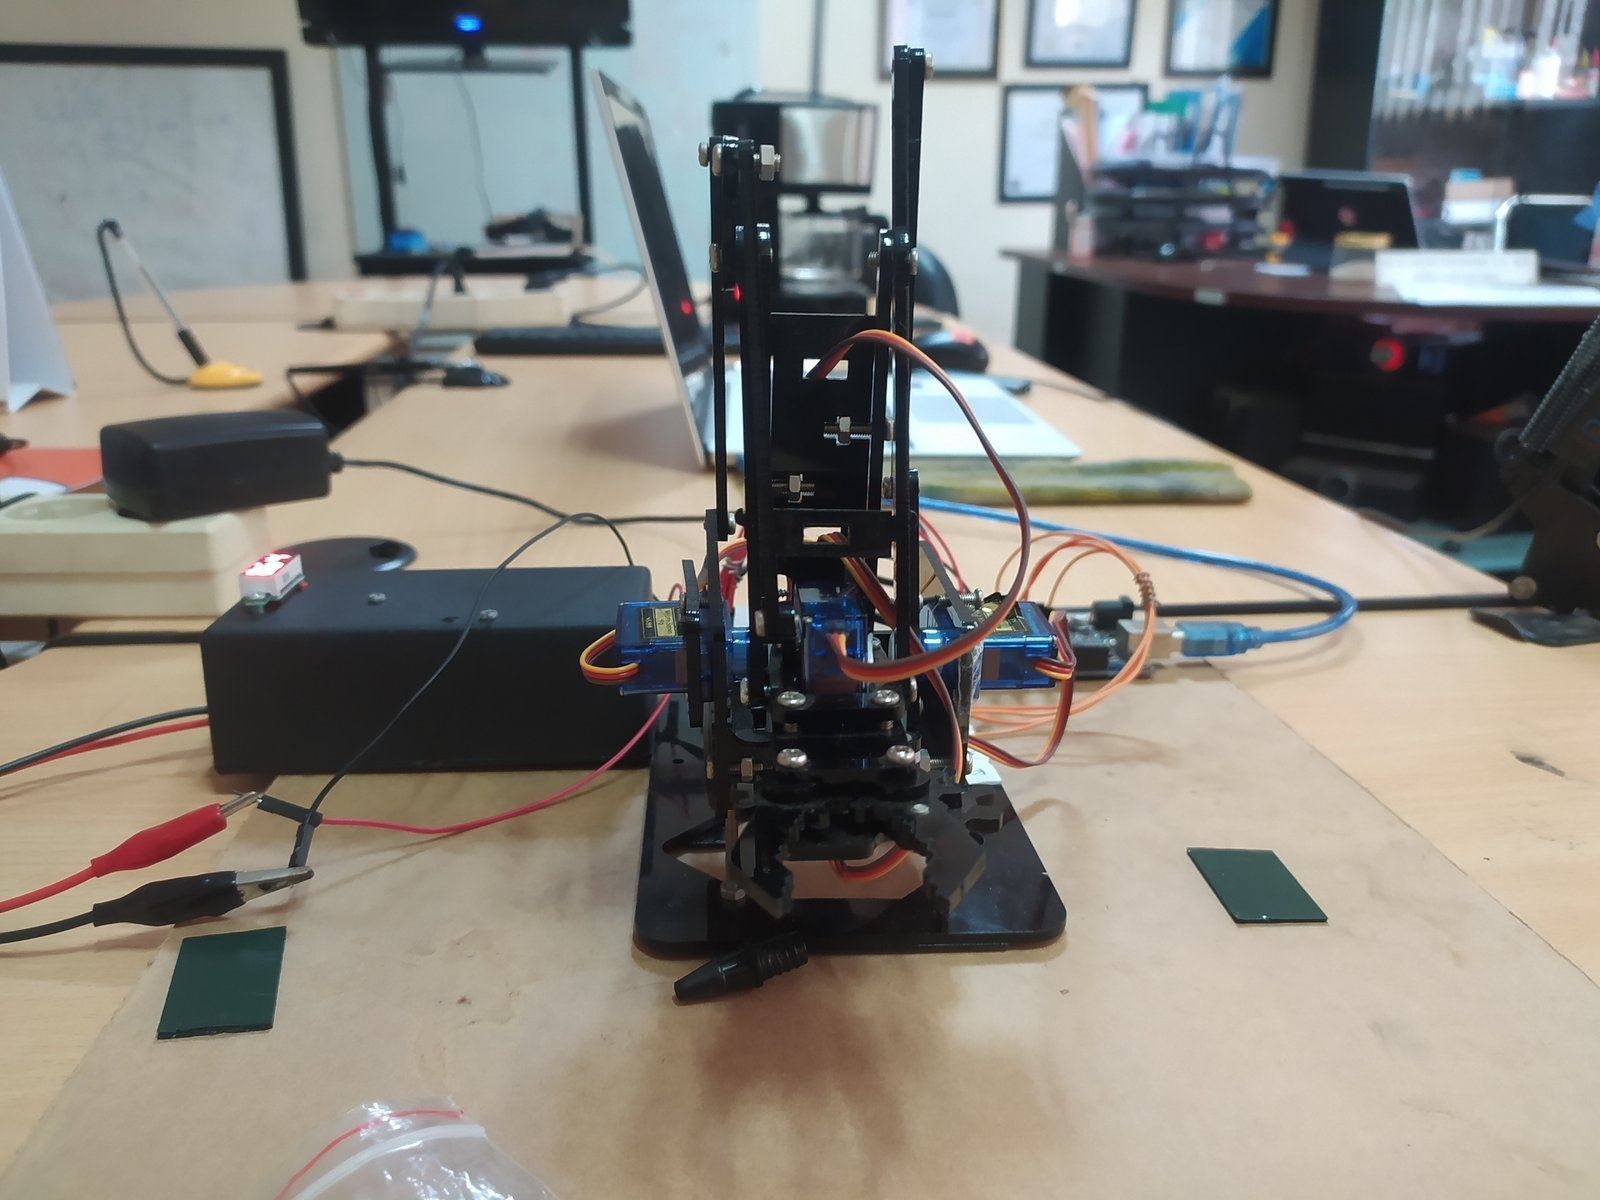
\includegraphics[width=\textwidth]{Gambar/Gambar6_1_mearm_tampak_depan.jpg}
        \caption{Purwarupa meArm (Tampak Depan)}
        \label{fig:app_6_1}
    \end{subfigure}
    \hfill
    \begin{subfigure}[b]{0.48\textwidth}
        \centering
        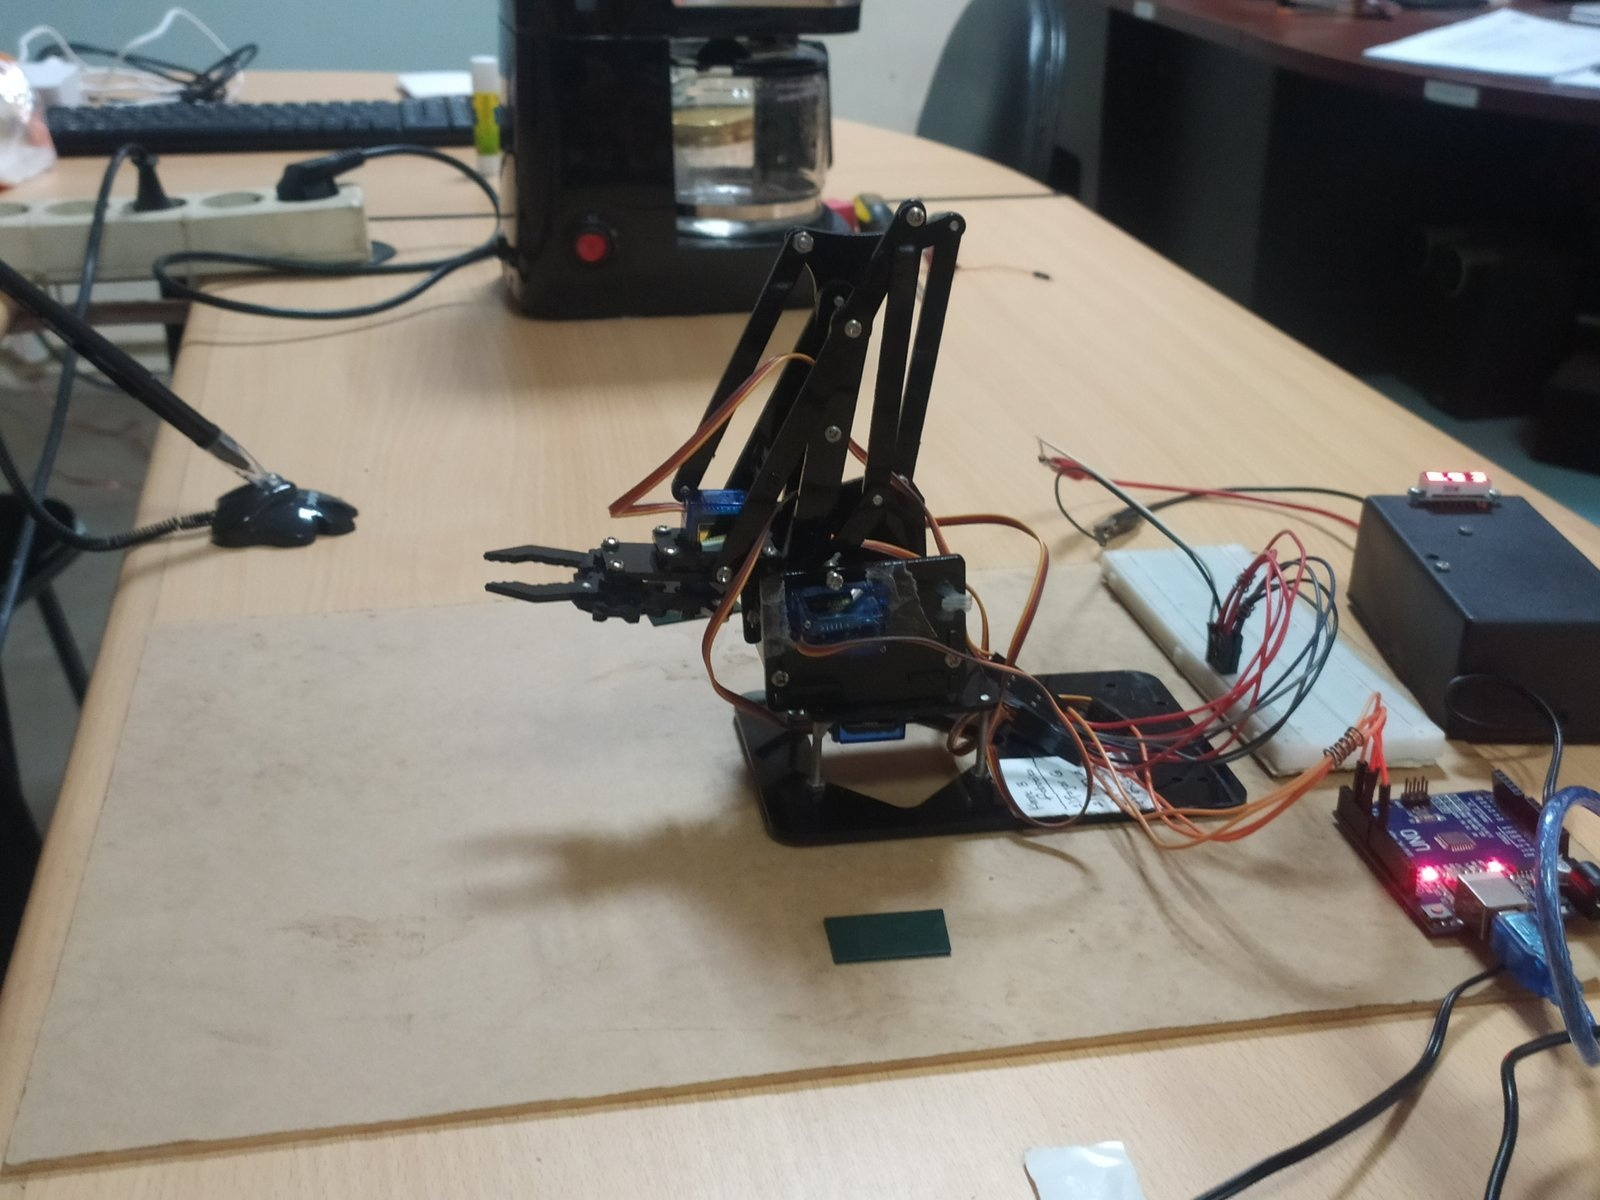
\includegraphics[width=\textwidth]{Gambar/Gambar6_2_mearm_dan_mikrokontroler.jpg}
        \caption{meArm dan Mikrokontroler}
        \label{fig:app_6_2}
    \end{subfigure}
    \caption{Dokumentasi Fisik Purwarupa meArm 4-DOF}
\end{figure}

\begin{figure}[htbp]
    \centering
    \begin{subfigure}[b]{0.48\textwidth}
        \centering
        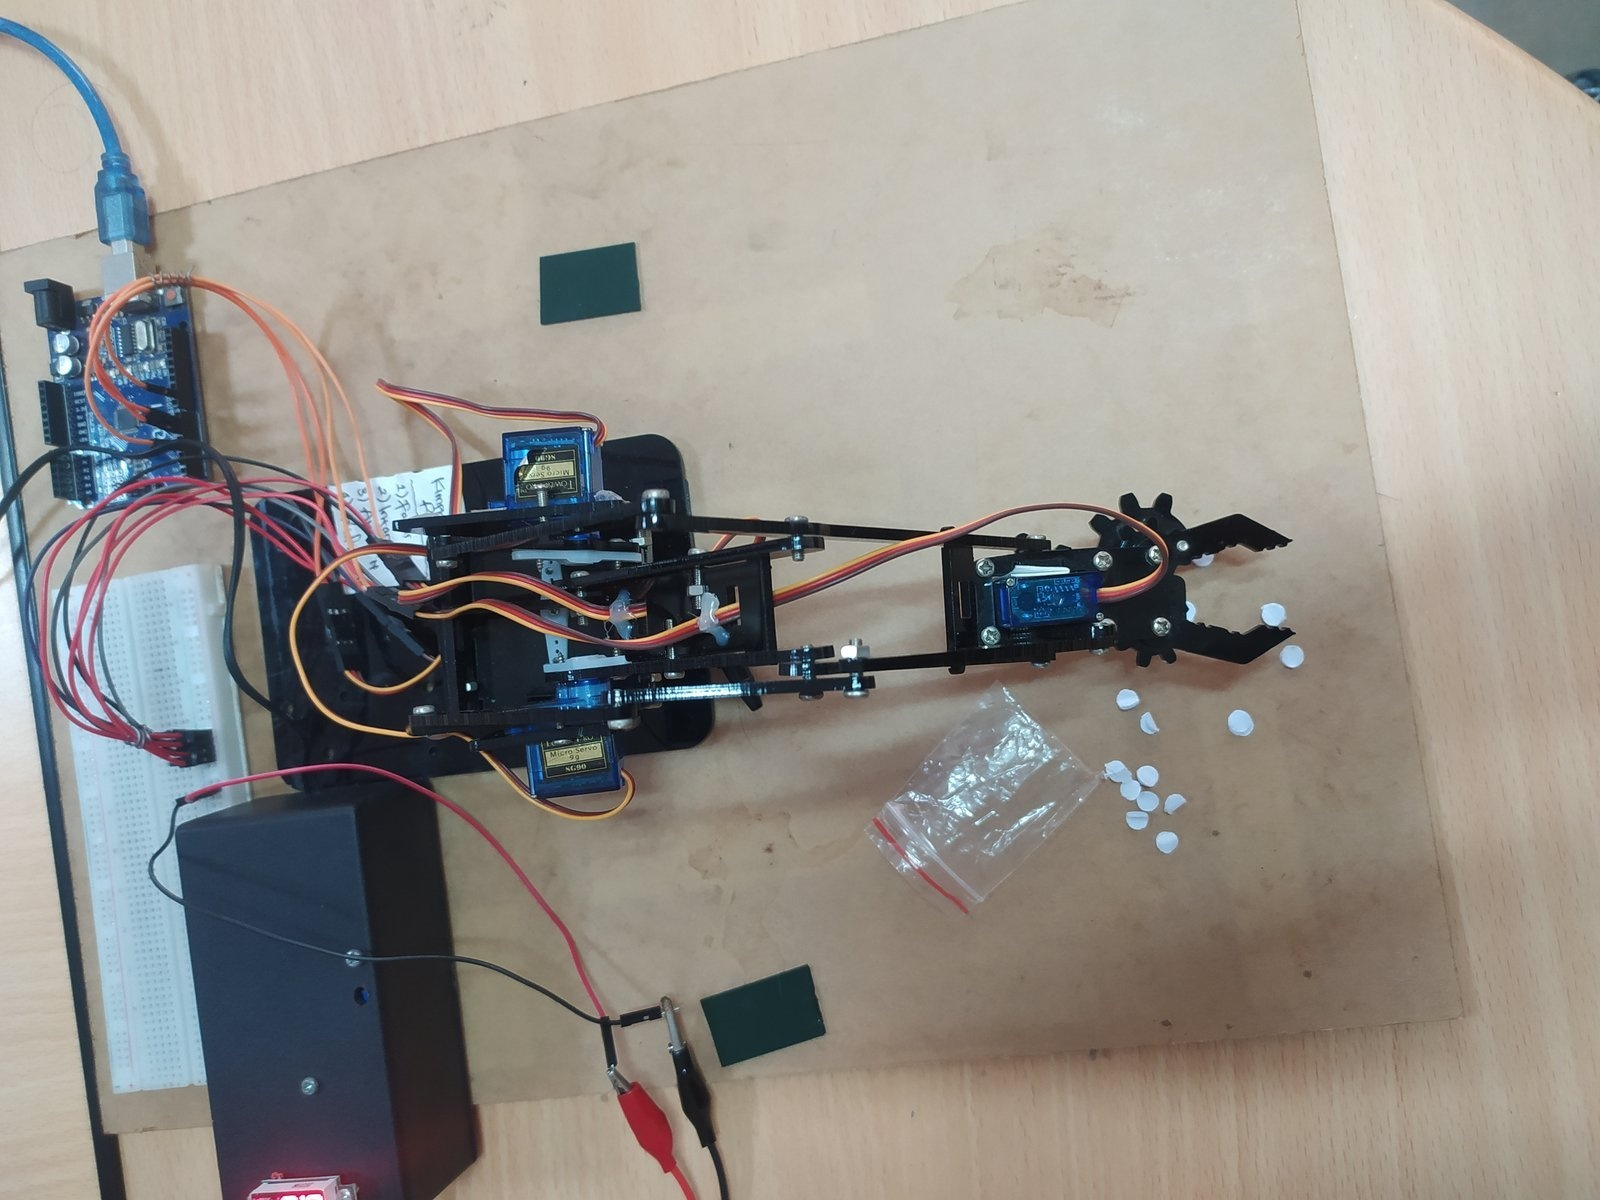
\includegraphics[width=\textwidth]{Gambar/Gambar6_3_mearm_tampak_atas.jpg}
        \caption{Purwarupa meArm (Tampak Atas)}
        \label{fig:app_6_3}
    \end{subfigure}
    \hfill
    \begin{subfigure}[b]{0.48\textwidth}
        \centering
        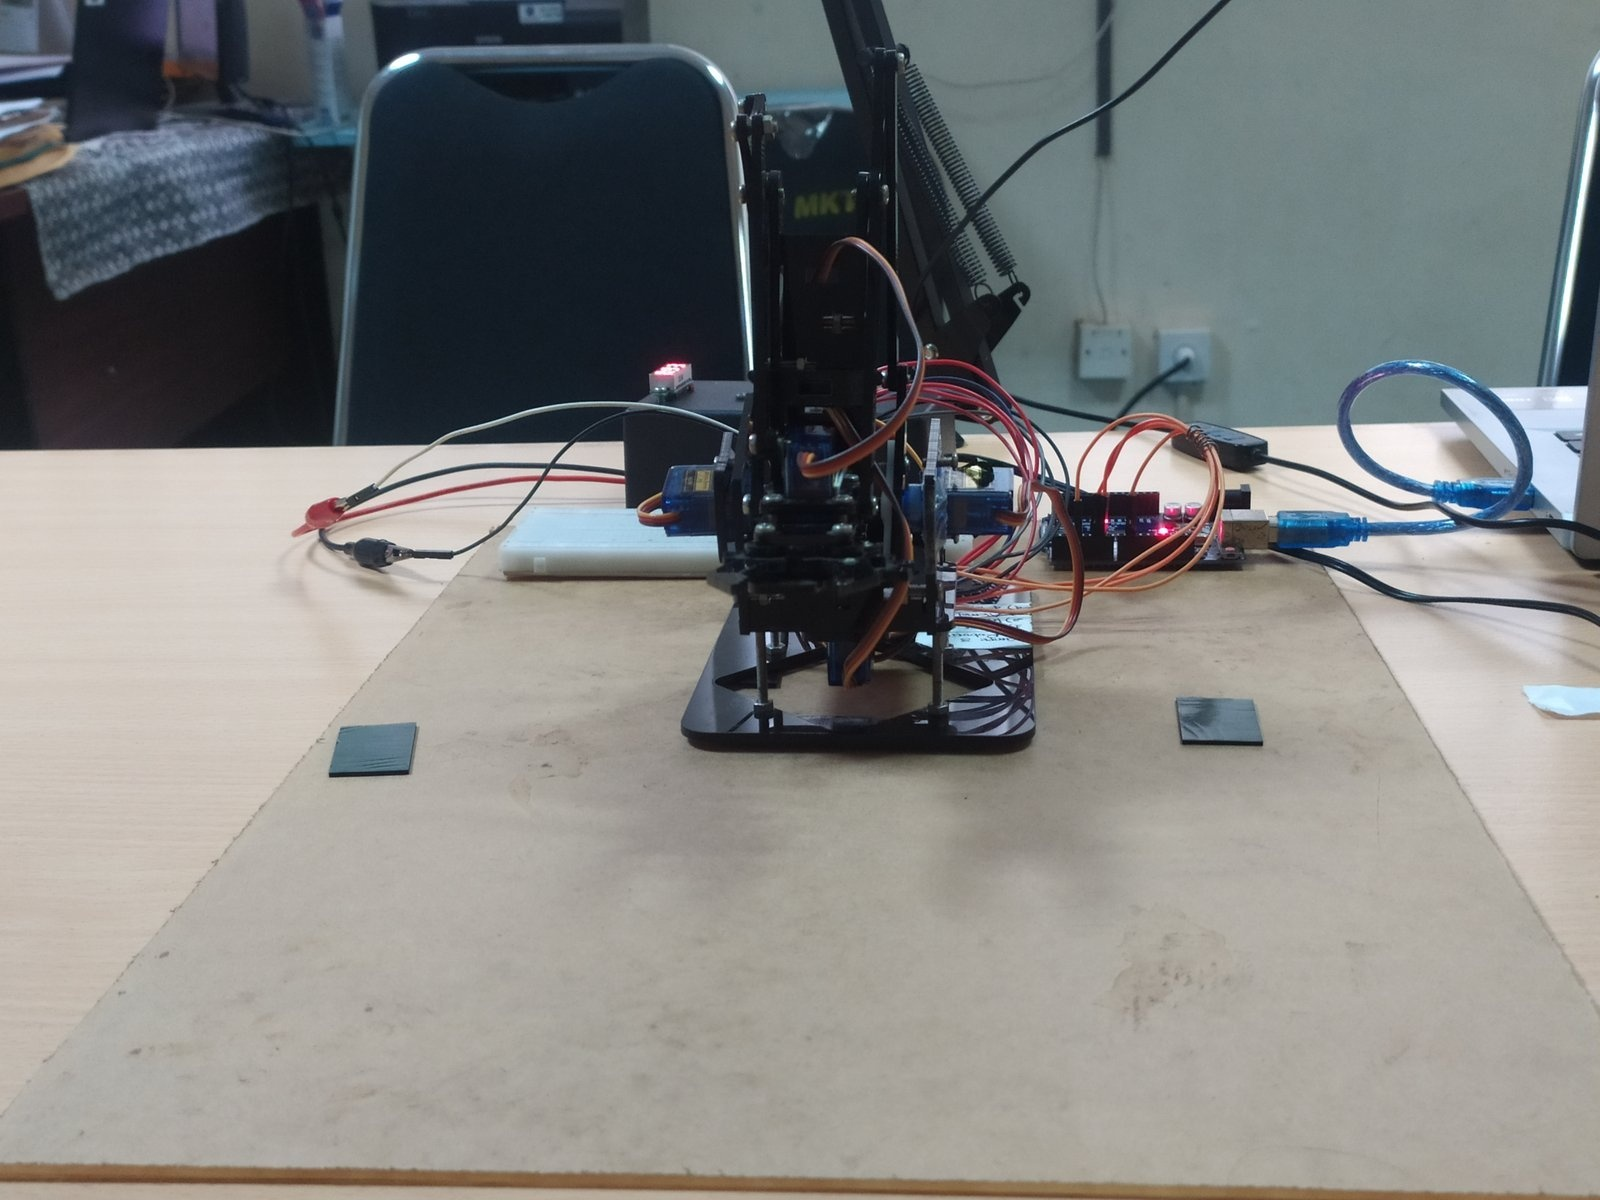
\includegraphics[width=\textwidth]{Gambar/Gambar6_4_mearm_sudut_depan_alternatif.jpg}
        \caption{meArm (Sudut Alternatif)}
        \label{fig:app_6_4}
    \end{subfigure}
    \caption{Dokumentasi Sudut Pandang Lengan meArm}
\end{figure}

\begin{figure}[htbp]
    \centering
    \begin{subfigure}[b]{0.48\textwidth}
        \centering
        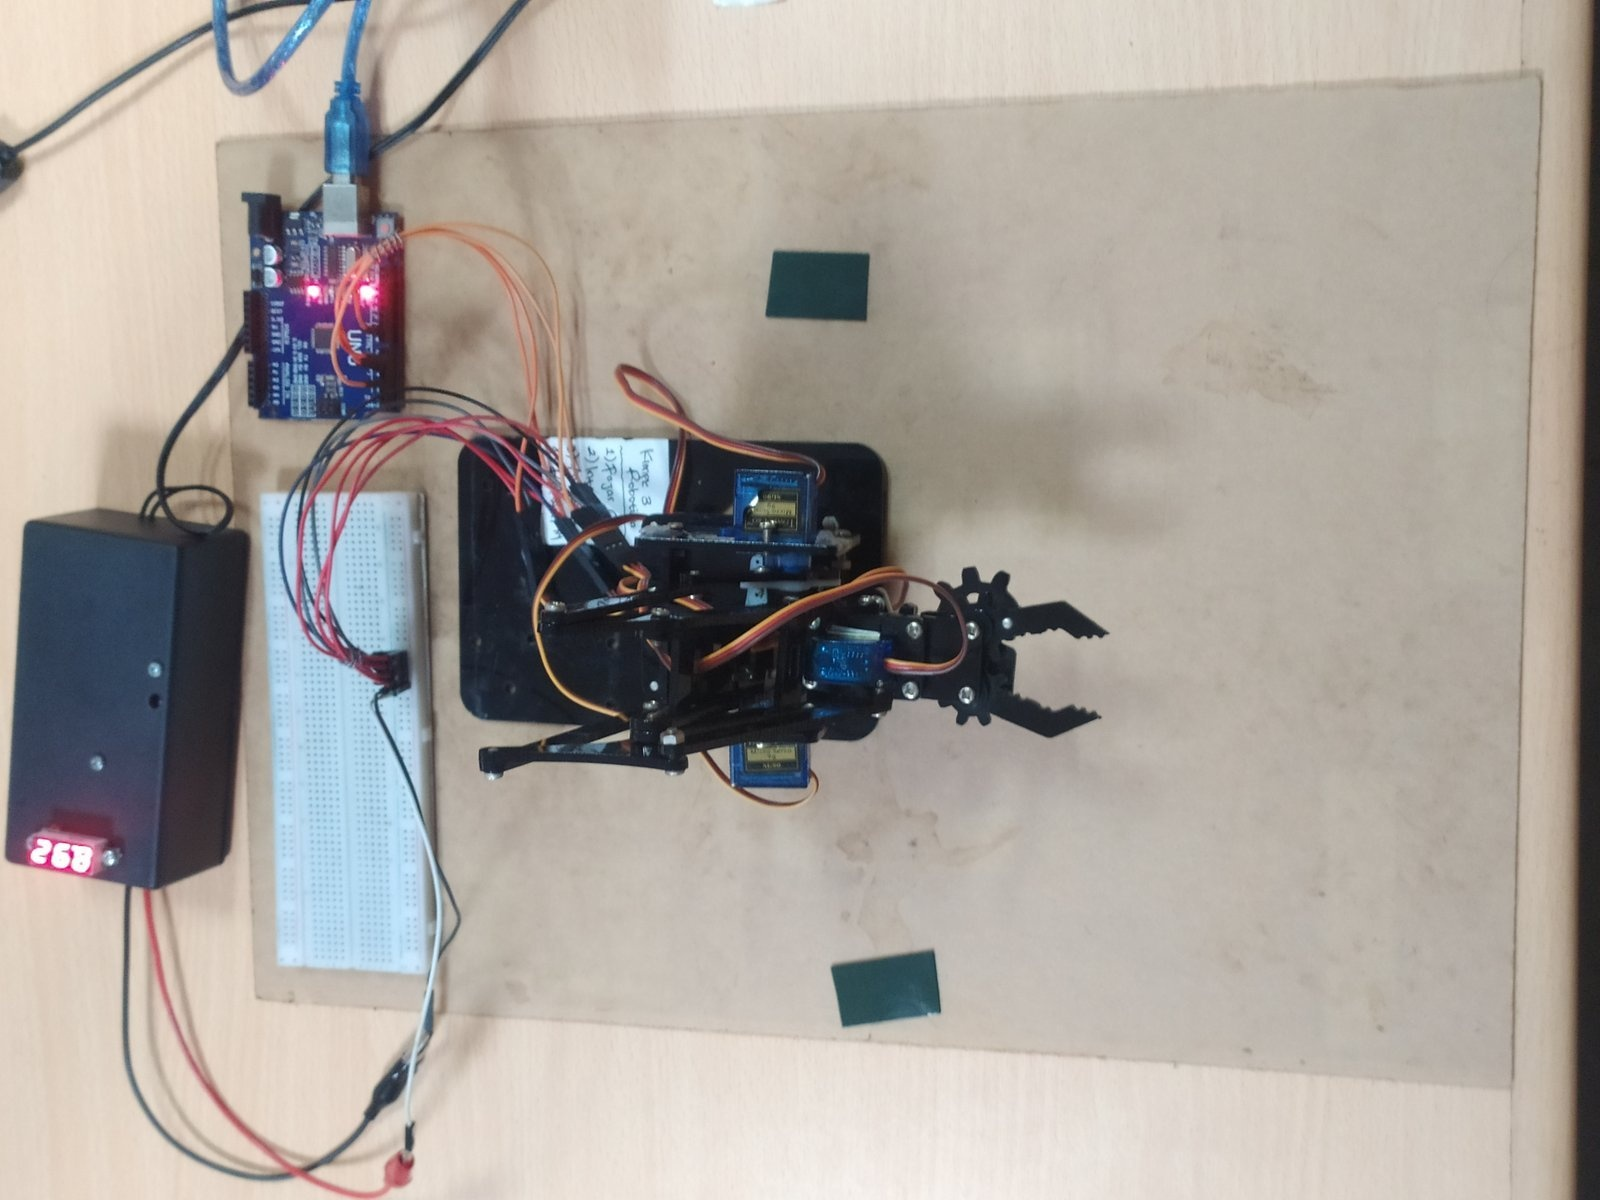
\includegraphics[width=\textwidth]{Gambar/Gambar6_5_perakitan_rangka_akrilik.jpg}
        \caption{Perakitan Rangka Akrilik}
        \label{fig:app_6_5}
    \end{subfigure}
    \hfill
    \begin{subfigure}[b]{0.48\textwidth}
        \centering
        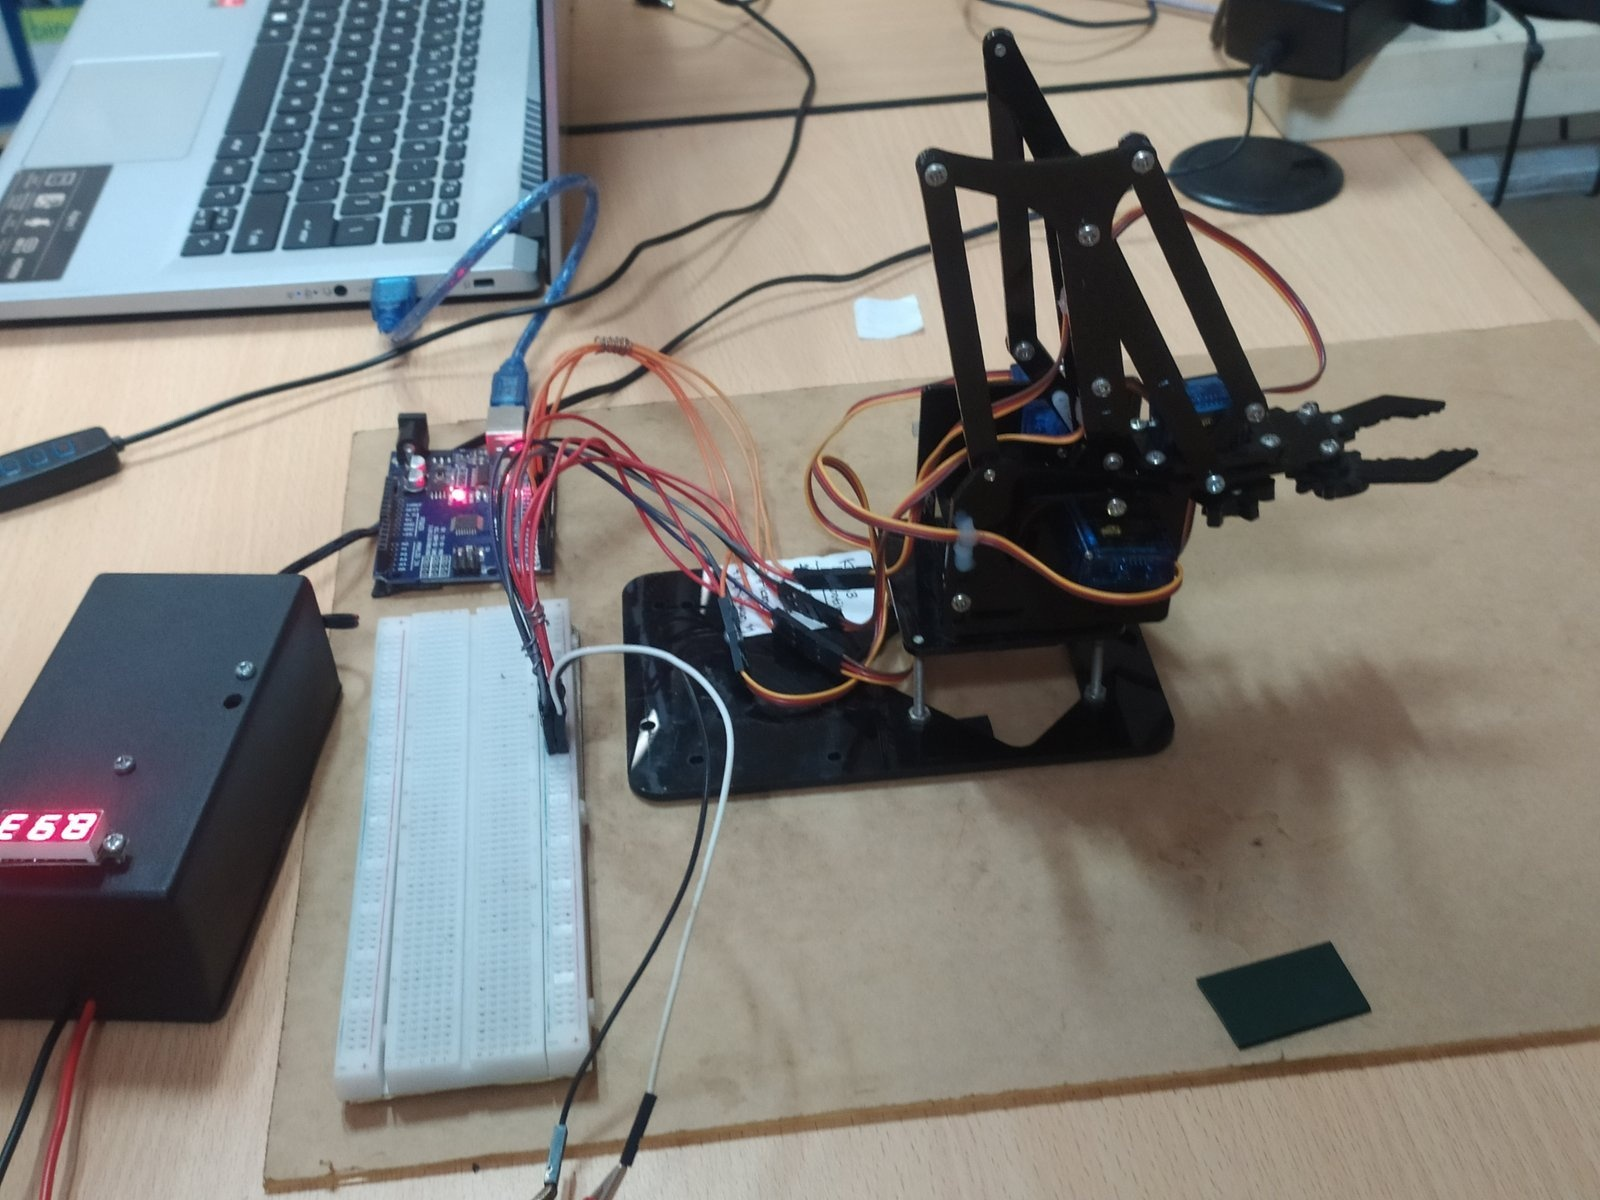
\includegraphics[width=\textwidth]{Gambar/Gambar6_6_penataan_pengkabelan_servo.jpg}
        \caption{Penataan Pengkabelan Servo}
        \label{fig:app_6_6}
    \end{subfigure}
    \caption{Proses Perakitan dan Pengkabelan meArm}
\end{figure}

\begin{figure}[htbp]
    \centering
    \begin{subfigure}[b]{0.48\textwidth}
        \centering
        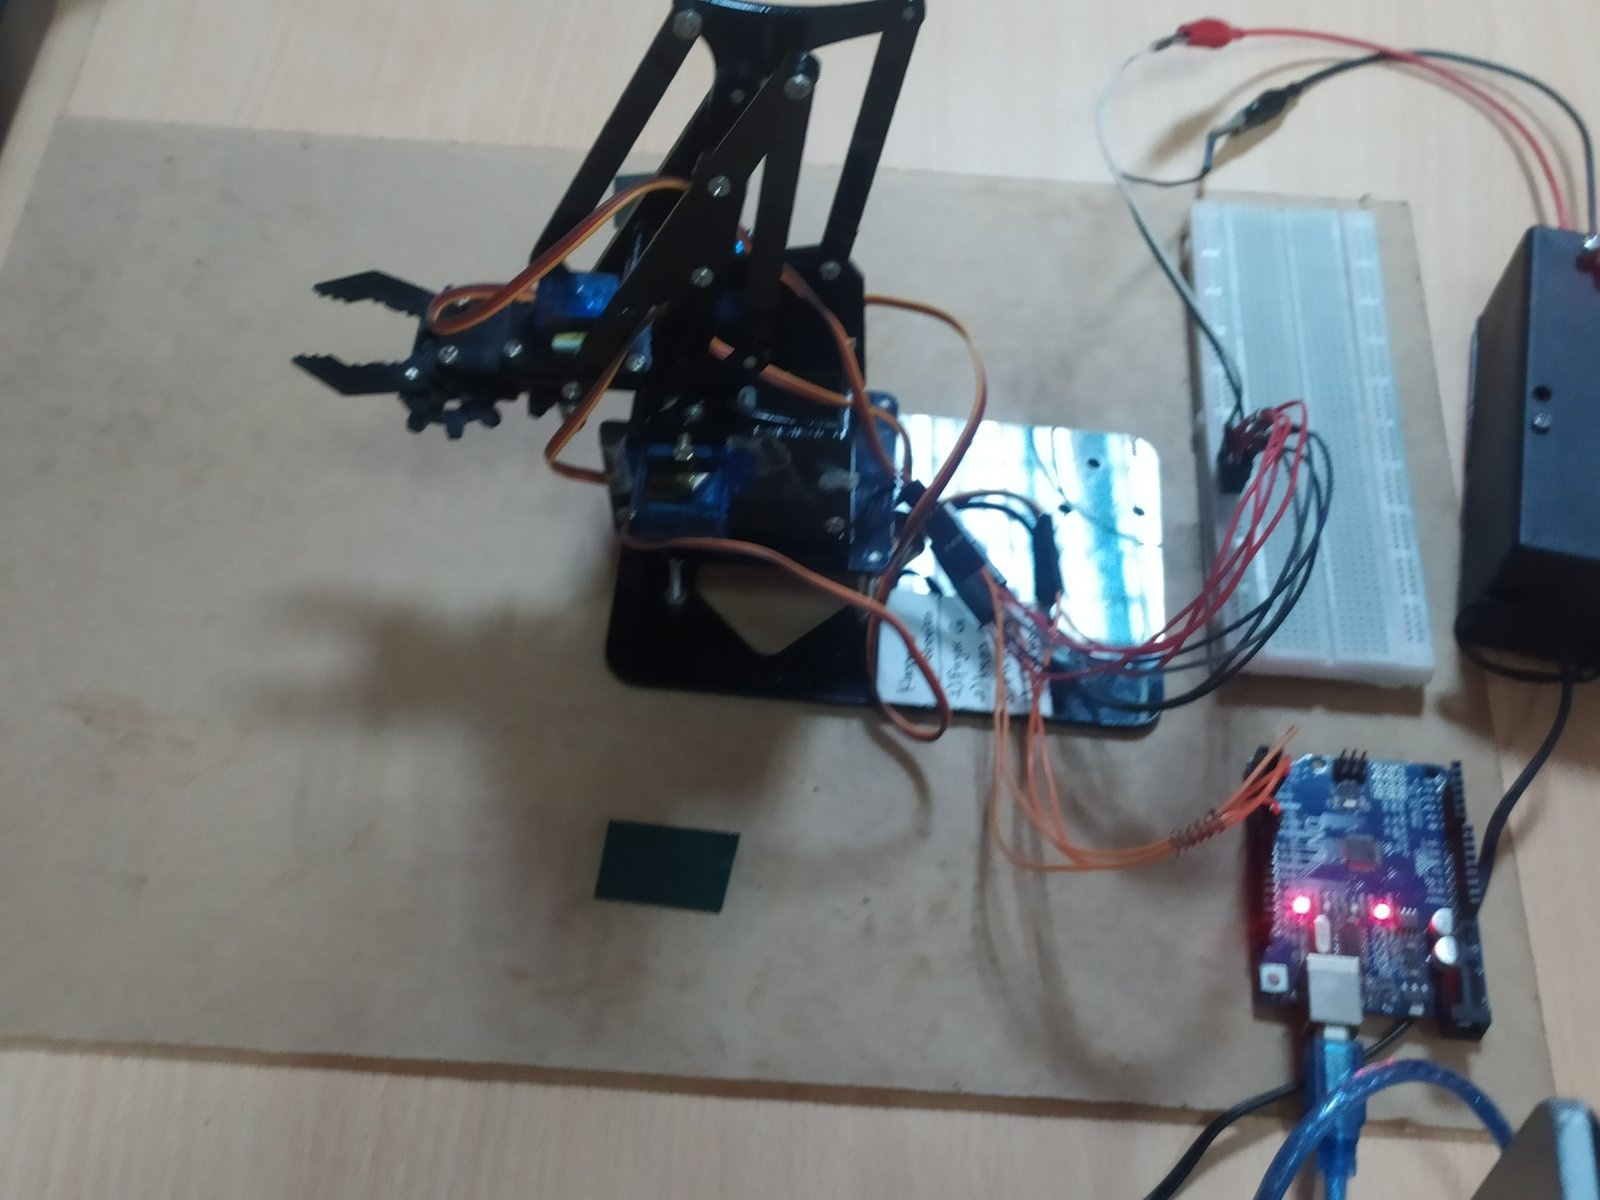
\includegraphics[width=\textwidth]{Gambar/Gambar6_7_detail_sambungan_tautan.jpg}
        \caption{Detail Sambungan Tautan Mekanika}
        \label{fig:app_6_7}
    \end{subfigure}
    \hfill
    \begin{subfigure}[b]{0.48\textwidth}
        \centering
        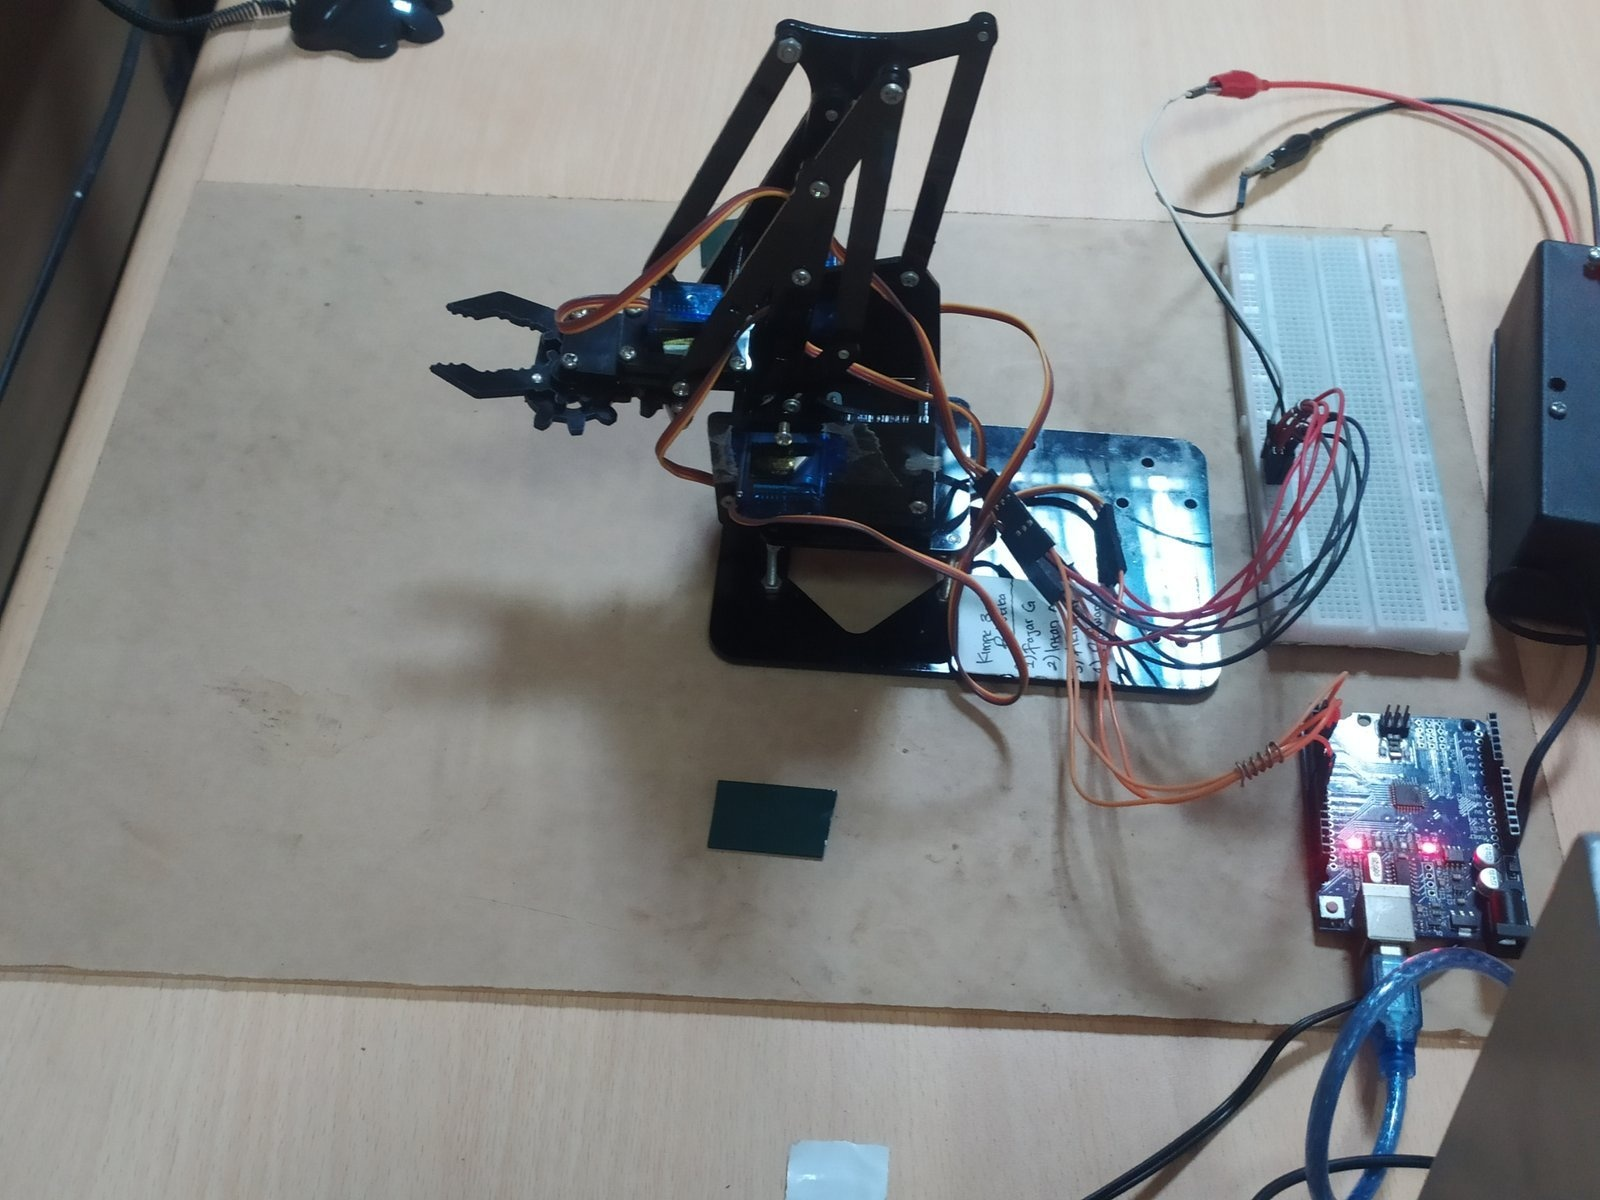
\includegraphics[width=\textwidth]{Gambar/Gambar6_8_pengujian_fleksibilitas_sendi.jpg}
        \caption{Pengujian Fleksibilitas Sendi}
        \label{fig:app_6_8}
    \end{subfigure}
    \caption{Pemeriksaan Mekanika Sambungan meArm}
\end{figure}

\begin{figure}[htbp]
    \centering
    \begin{subfigure}[b]{0.48\textwidth}
        \centering
        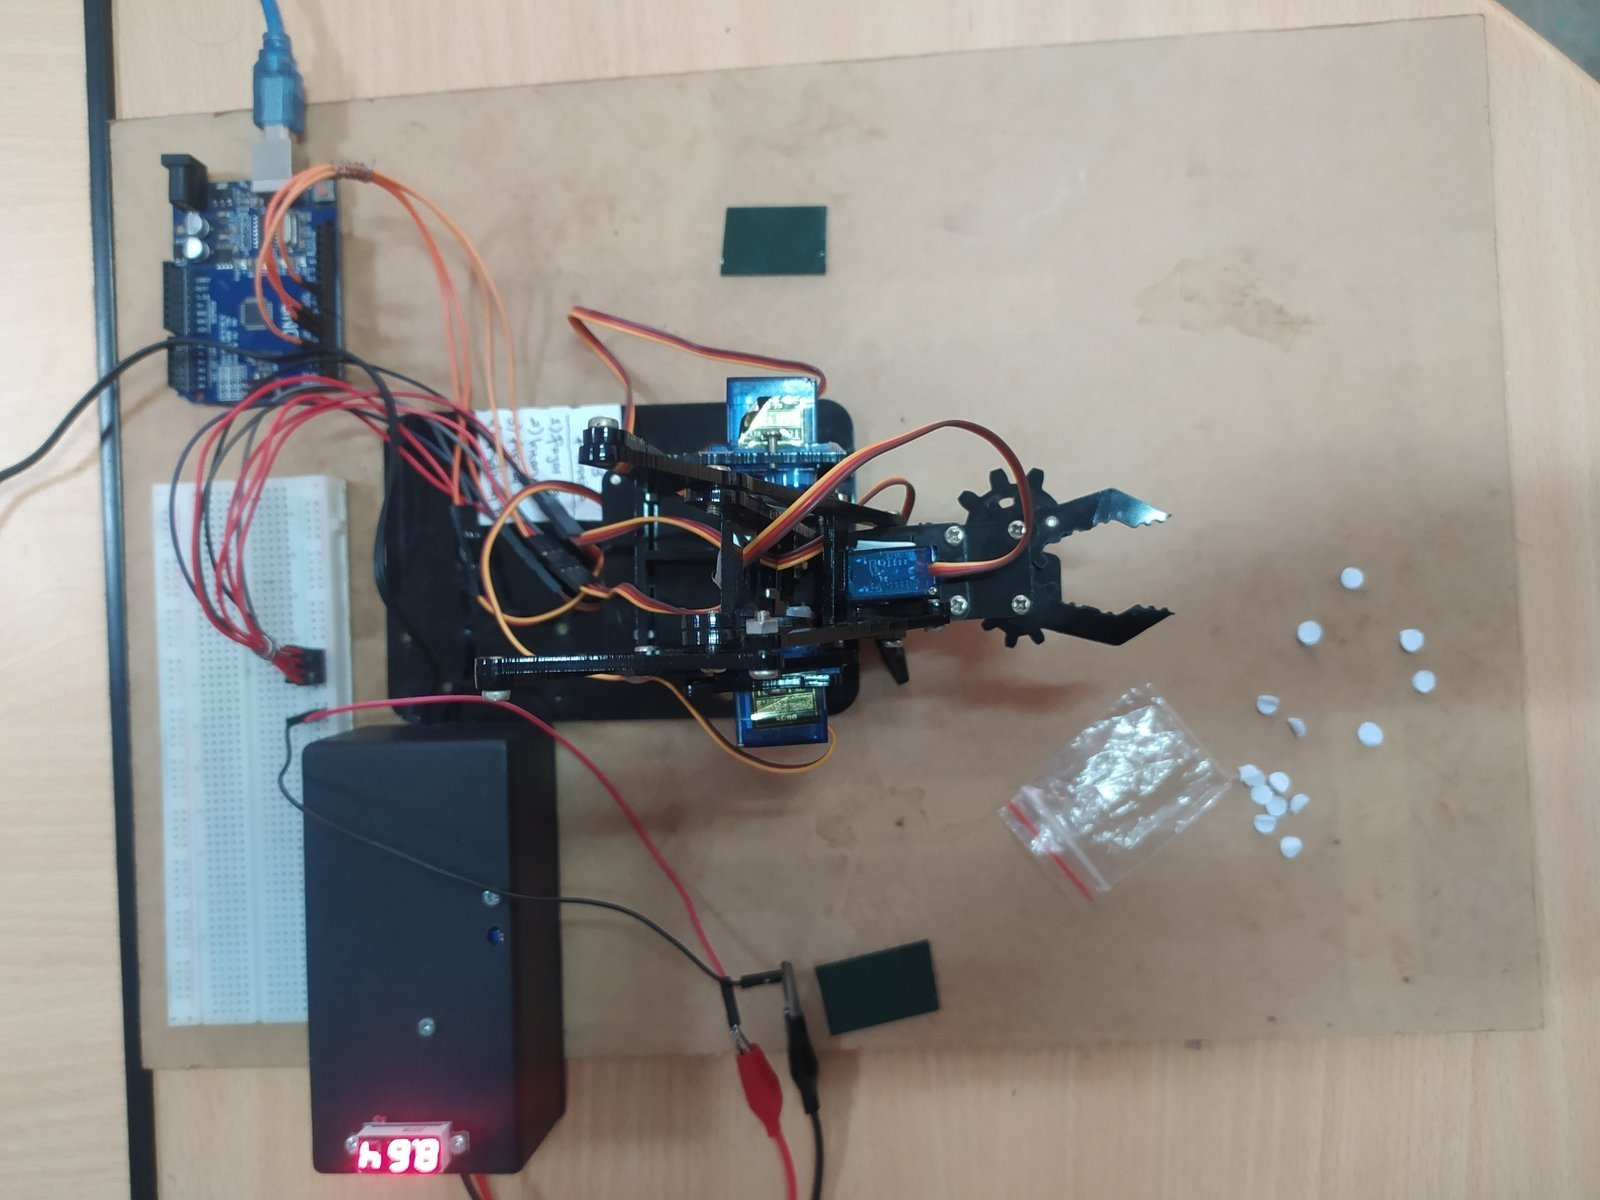
\includegraphics[width=\textwidth]{Gambar/Gambar6_9_integrasi_sistem_mearm.jpg}
        \caption{Integrasi Sistem di Meja Eksperimen}
        \label{fig:app_6_9}
    \end{subfigure}
    \hfill
    \begin{subfigure}[b]{0.48\textwidth}
        \centering
        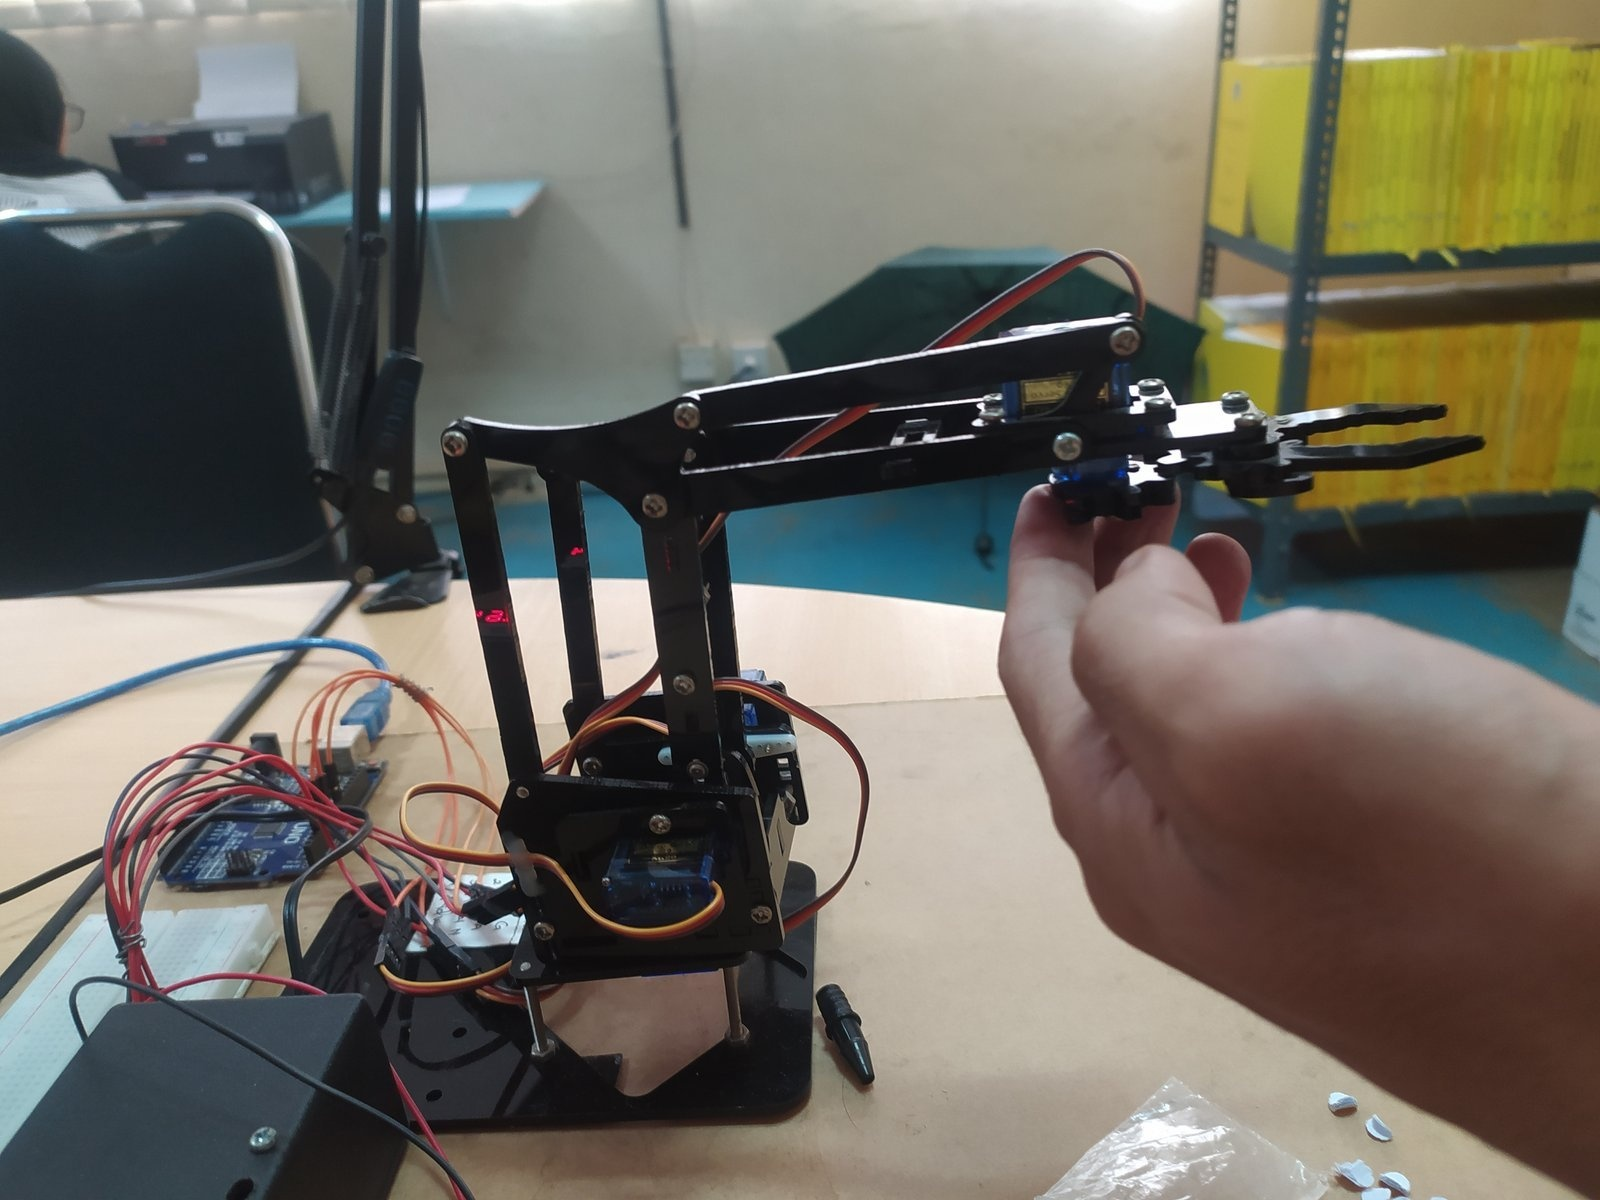
\includegraphics[width=\textwidth]{Gambar/Gambar6_10_pengujian_manuver_ik_sesi1.jpg}
        \caption{Uji Manuver Kinematika Balikan Sesi 1}
        \label{fig:app_6_10}
    \end{subfigure}
    \caption{Pengujian Eksperimental meArm}
\end{figure}

\begin{figure}[htbp]
    \centering
    \begin{subfigure}[b]{0.48\textwidth}
        \centering
        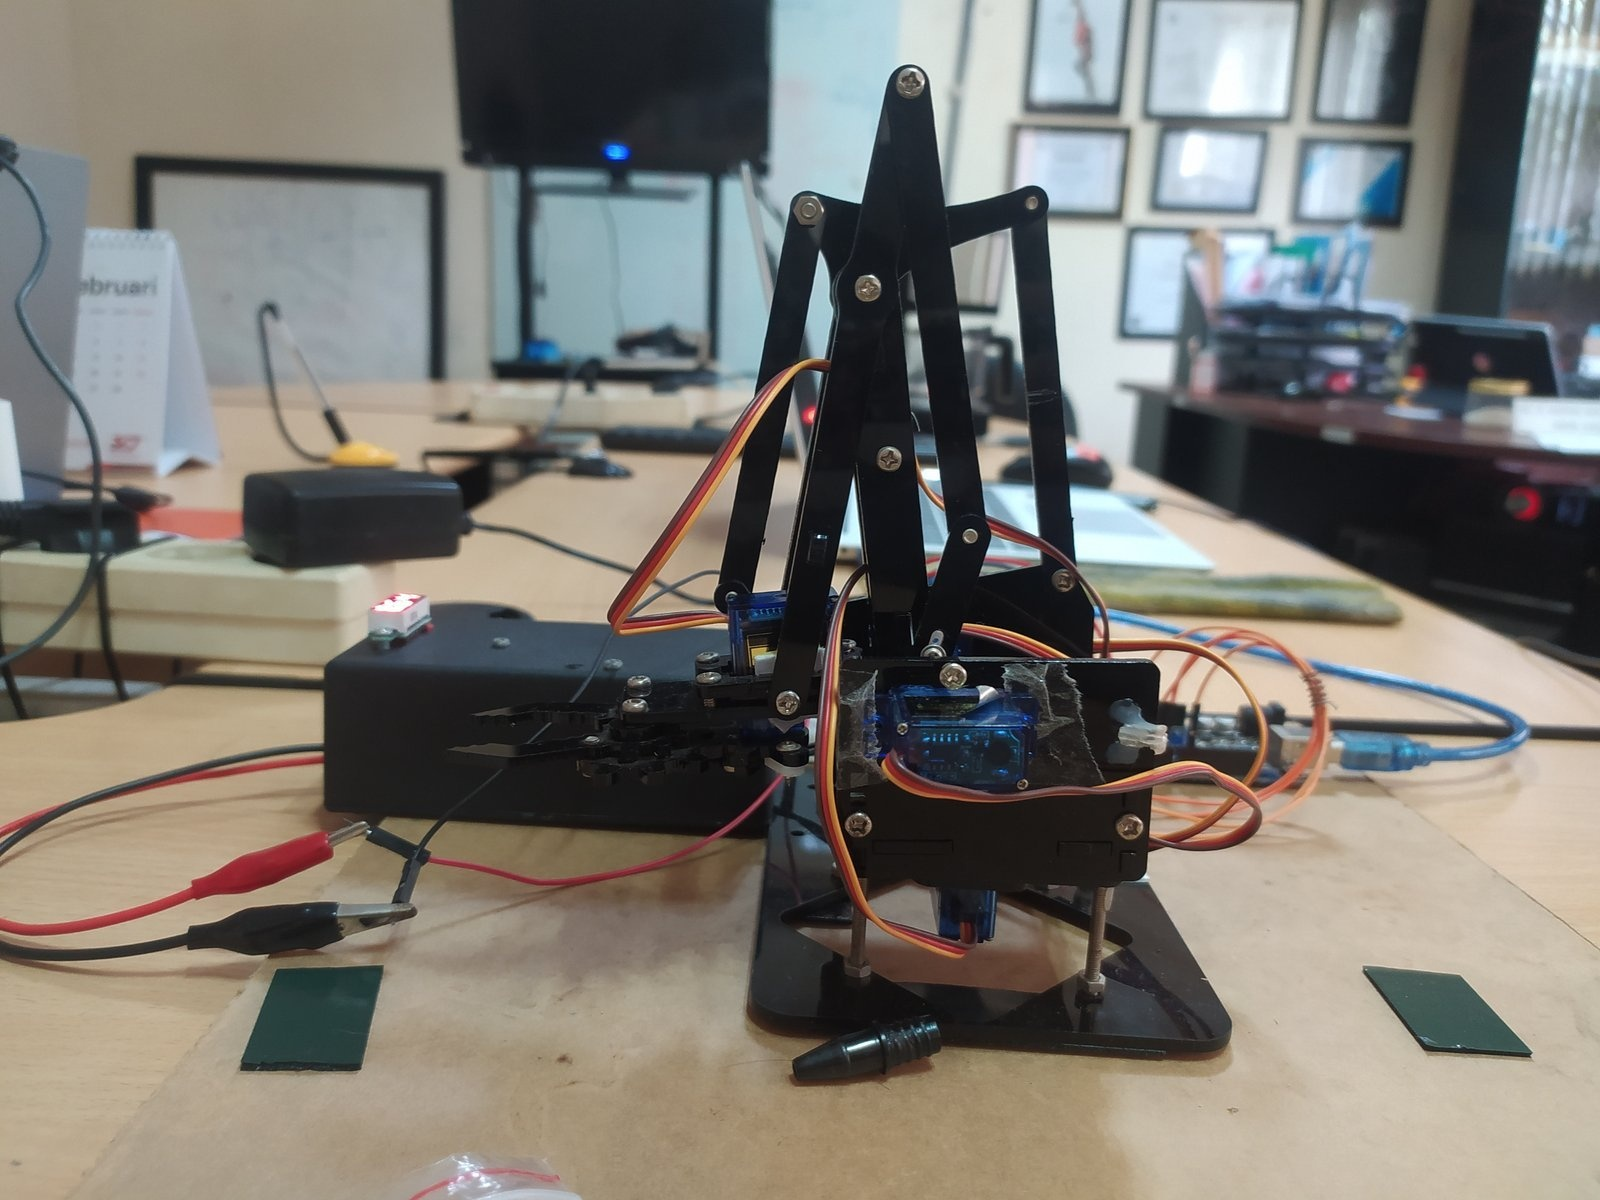
\includegraphics[width=\textwidth]{Gambar/Gambar6_11_pengujian_manuver_ik_sesi2.jpg}
        \caption{Uji Manuver Kinematika Balikan Sesi 2}
        \label{fig:app_6_11}
    \end{subfigure}
    \hfill
    \begin{subfigure}[b]{0.48\textwidth}
        \centering
        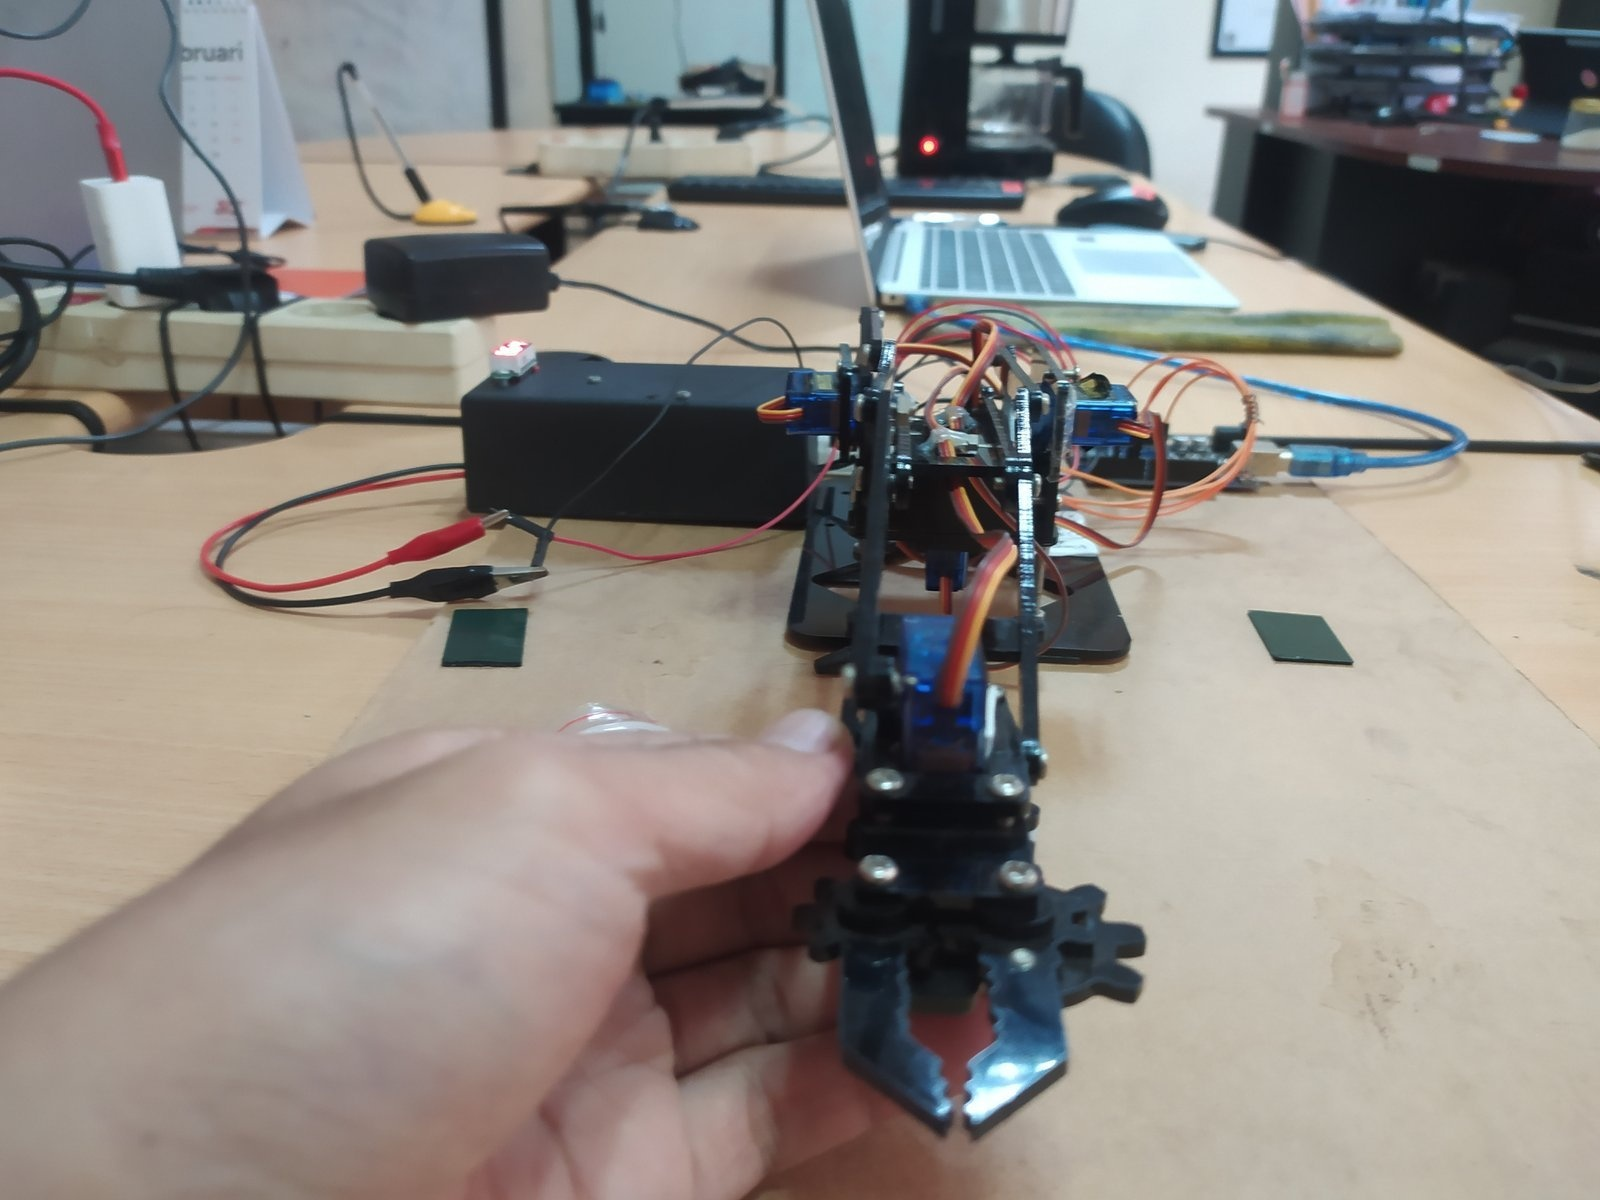
\includegraphics[width=\textwidth]{Gambar/Gambar6_12_pengujian_jangkauan_capit.jpg}
        \caption{Pengujian Jangkauan dan Capit}
        \label{fig:app_6_12}
    \end{subfigure}
    \caption{Pengujian Jangkauan Kerja dan Capit meArm}
\end{figure}

\begin{figure}[htbp]
    \centering
    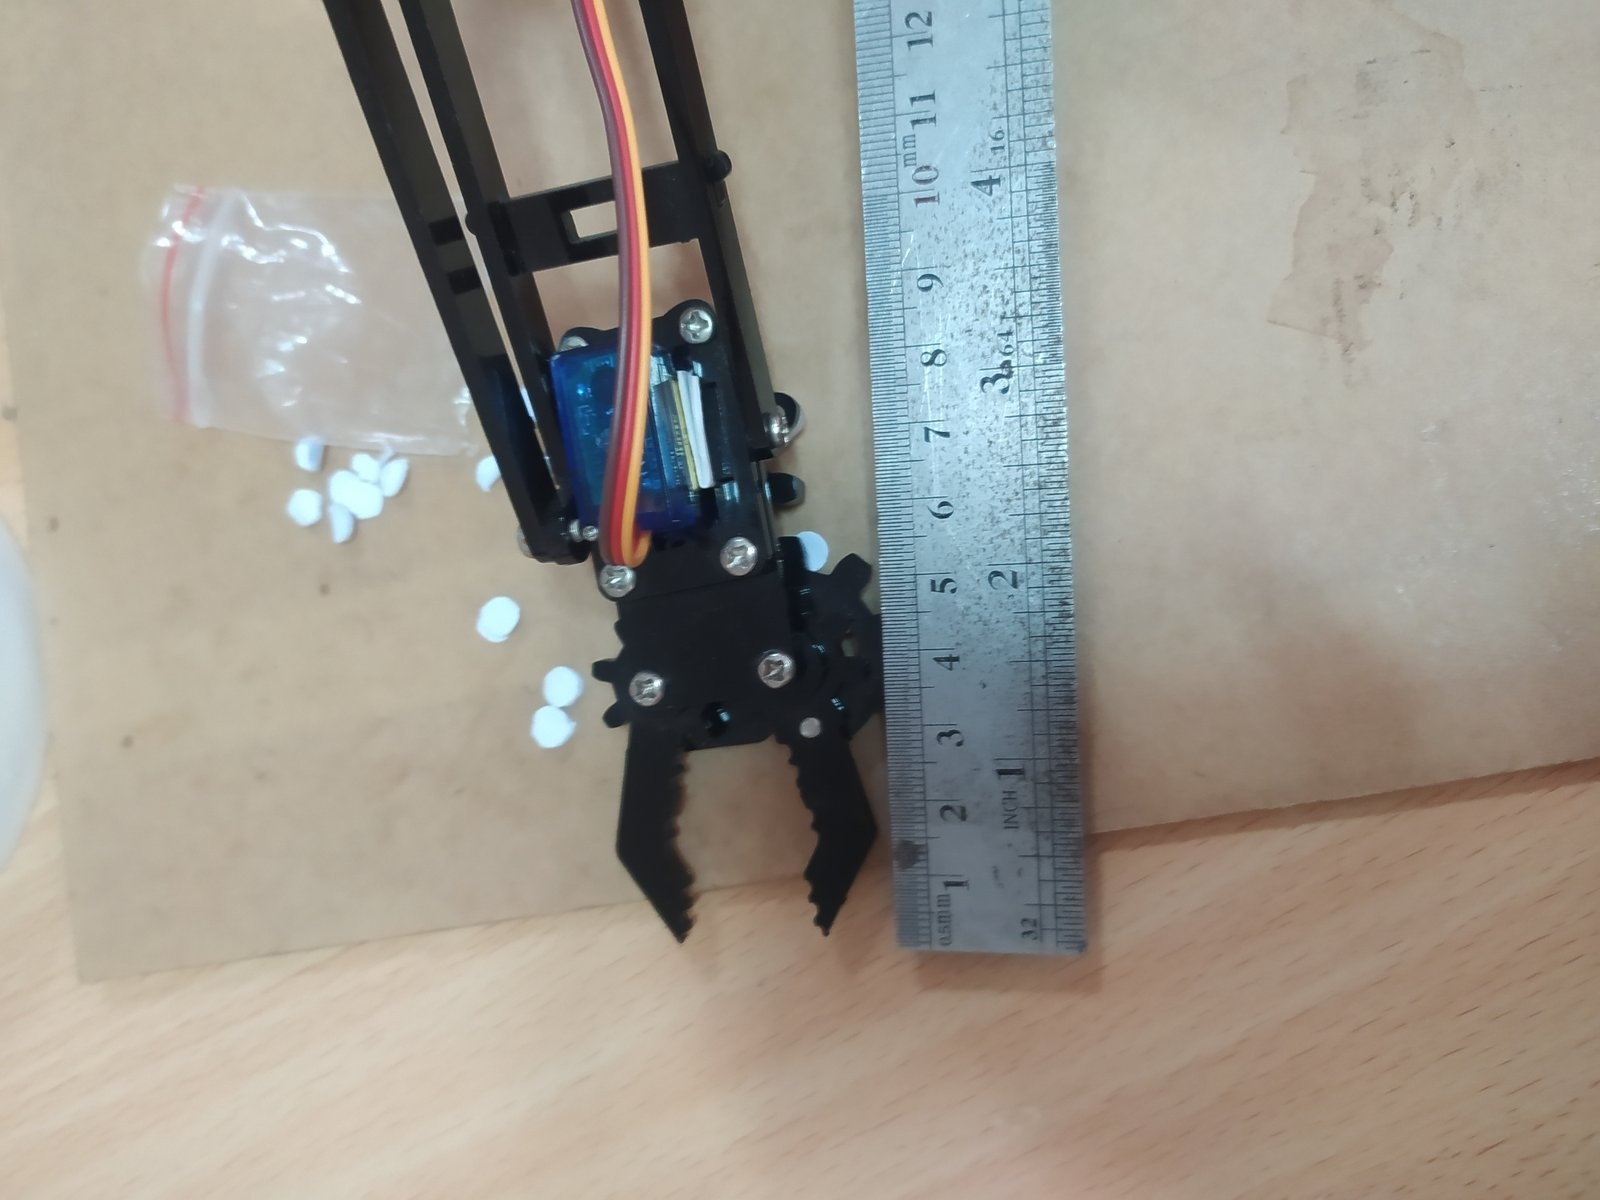
\includegraphics[width=0.75\textwidth]{Gambar/Gambar6_13_pengujian_respons_gerak_sibi.jpg}
    \caption{Pengujian Respons Gerak meArm Berbasis Isyarat SIBI}
    \label{fig:app_6_13}
\end{figure}

\newpage
\subsection*{4.2 Dokumentasi Perangkat dan Teleoperasi Dobot Magician}

\begin{figure}[htbp]
    \centering
    \begin{subfigure}[b]{0.48\textwidth}
        \centering
        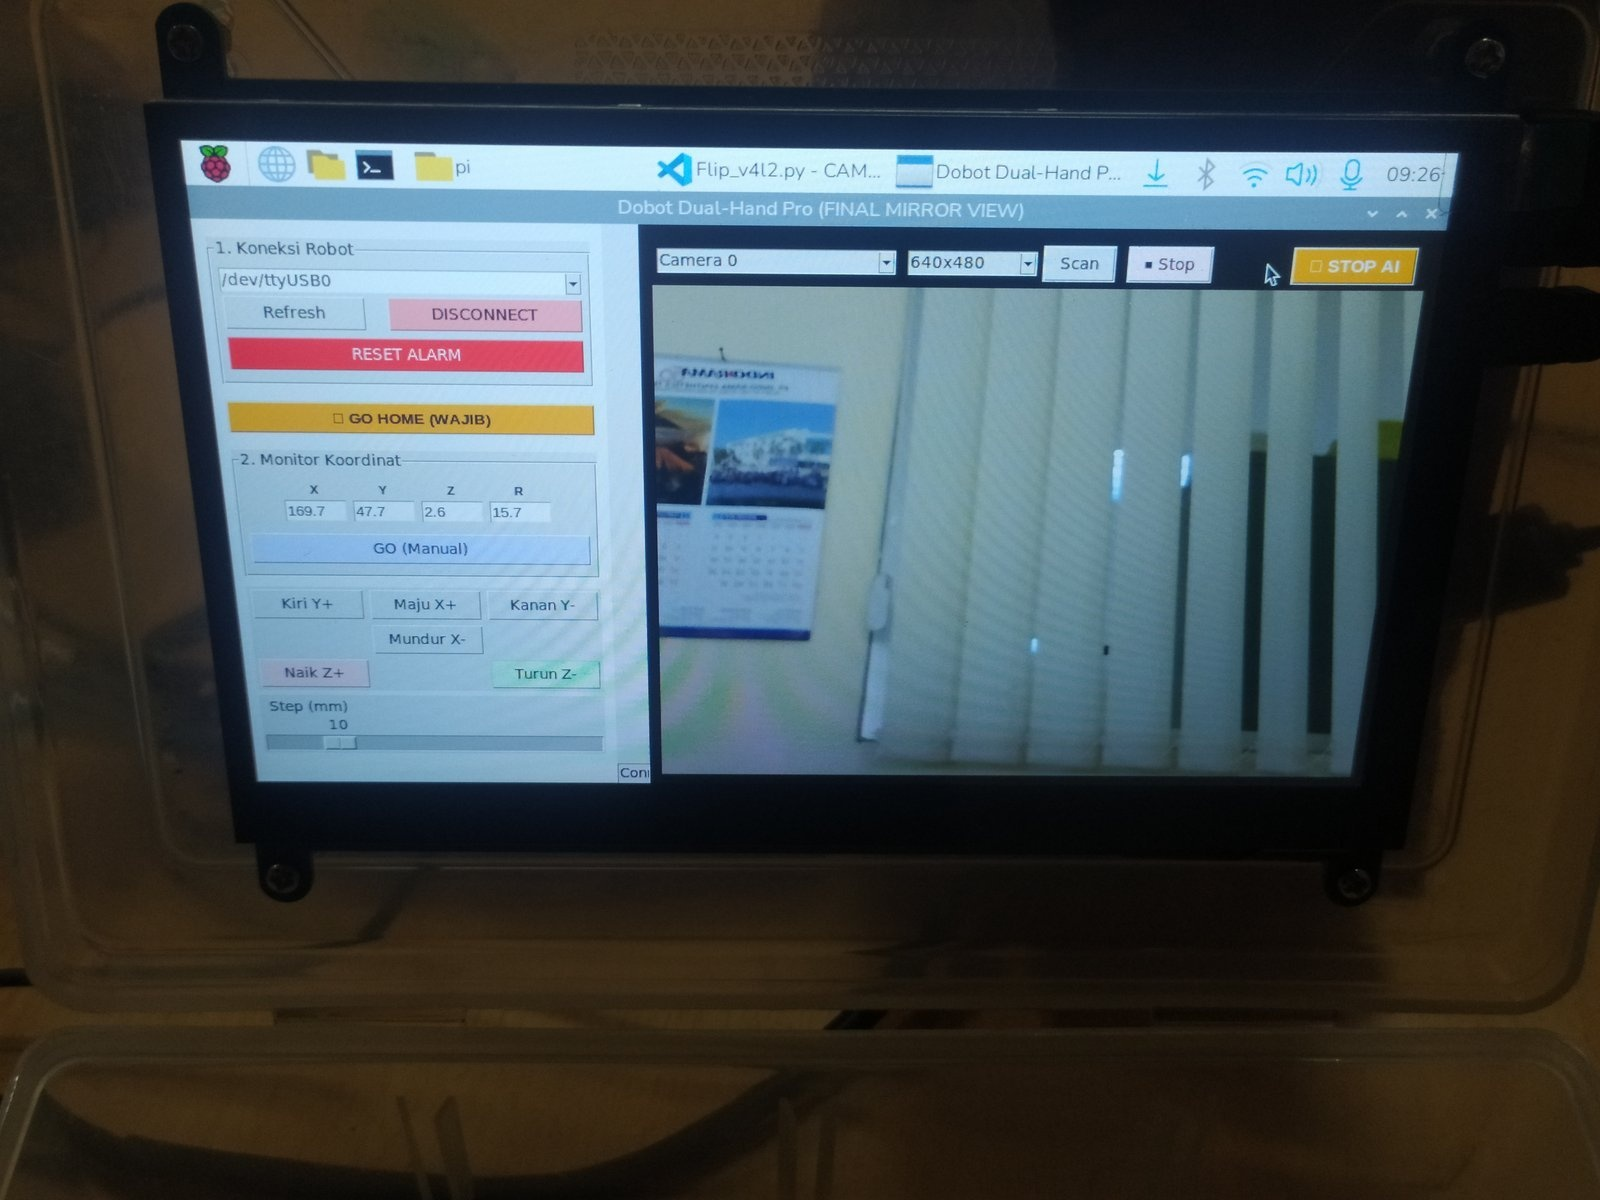
\includegraphics[width=\textwidth]{Gambar/Gambar6_14_antarmuka_pelacakan_dobot.jpg}
        \caption{Antarmuka Pelacakan Tangan}
        \label{fig:app_6_14}
    \end{subfigure}
    \hfill
    \begin{subfigure}[b]{0.48\textwidth}
        \centering
        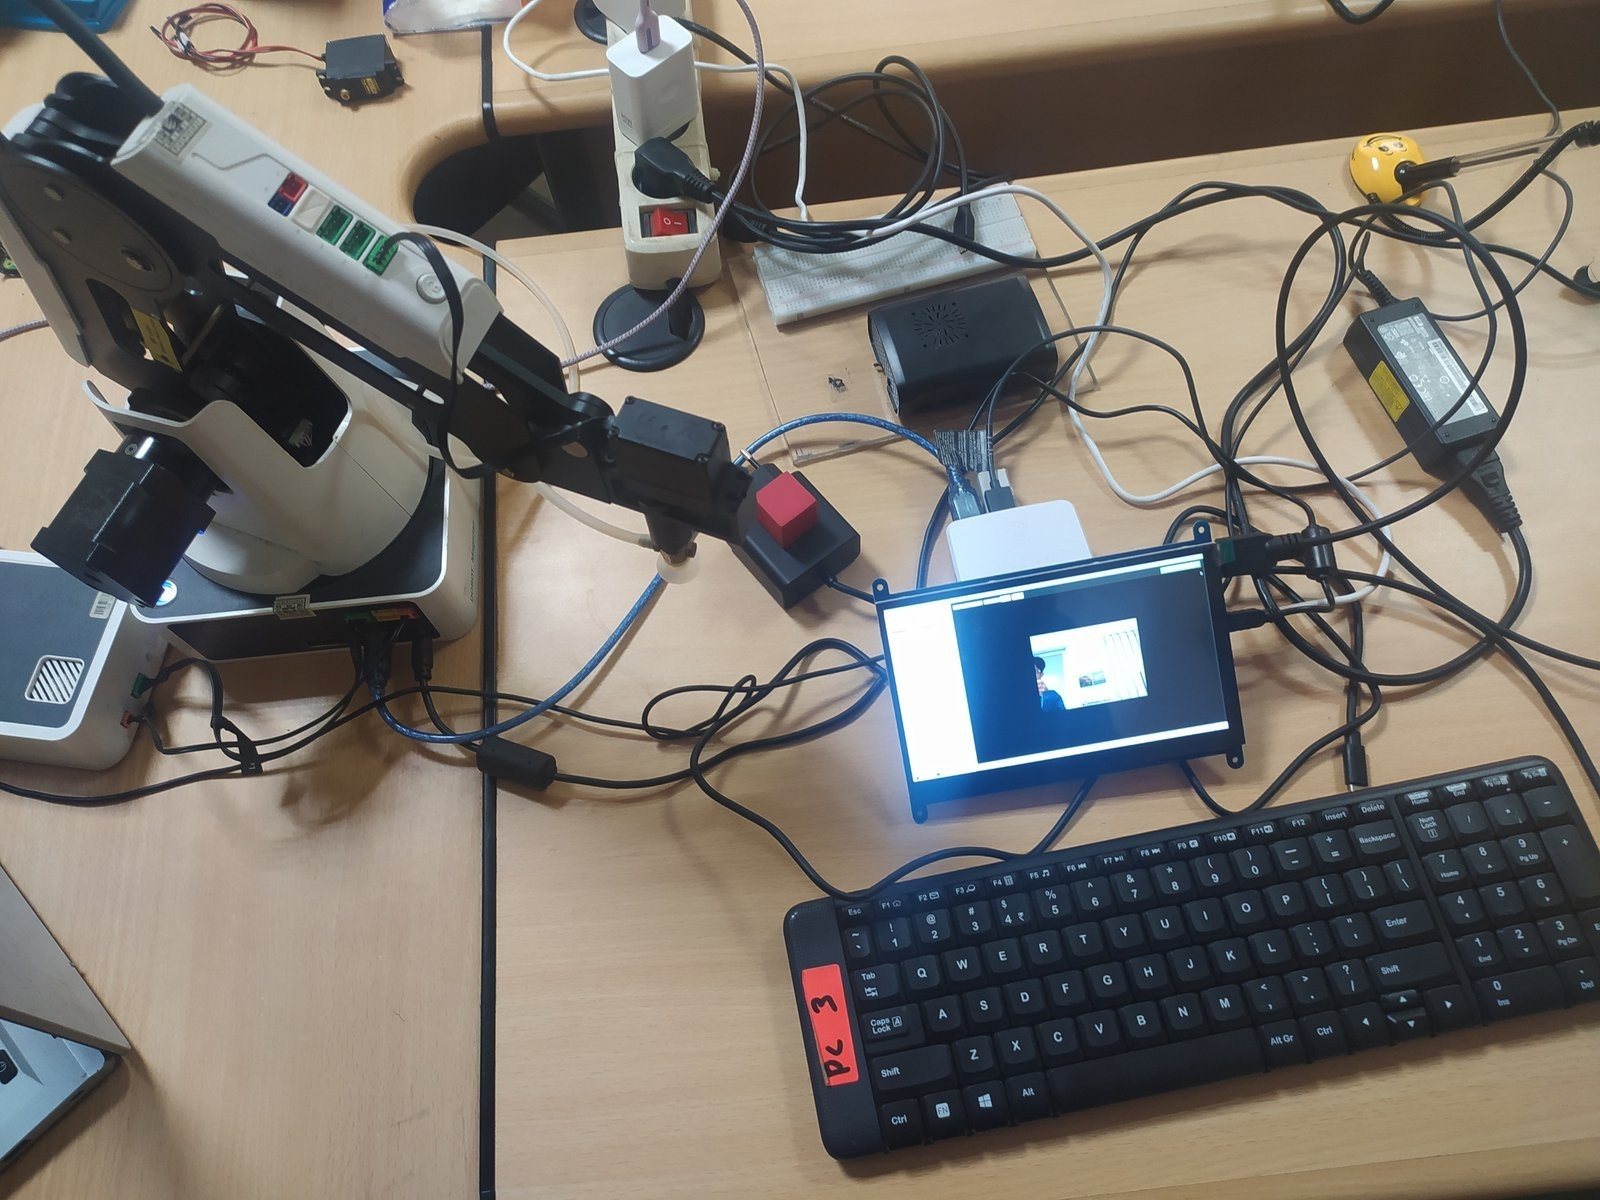
\includegraphics[width=\textwidth]{Gambar/Gambar6_15_stasiun_teleoperasi_dobot1.jpg}
        \caption{Stasiun Kerja Teleoperasi (Sudut 1)}
        \label{fig:app_6_15}
    \end{subfigure}
    \caption{Pengujian Teleoperasi Dobot Magician}
\end{figure}

\begin{figure}[htbp]
    \centering
    \begin{subfigure}[b]{0.48\textwidth}
        \centering
        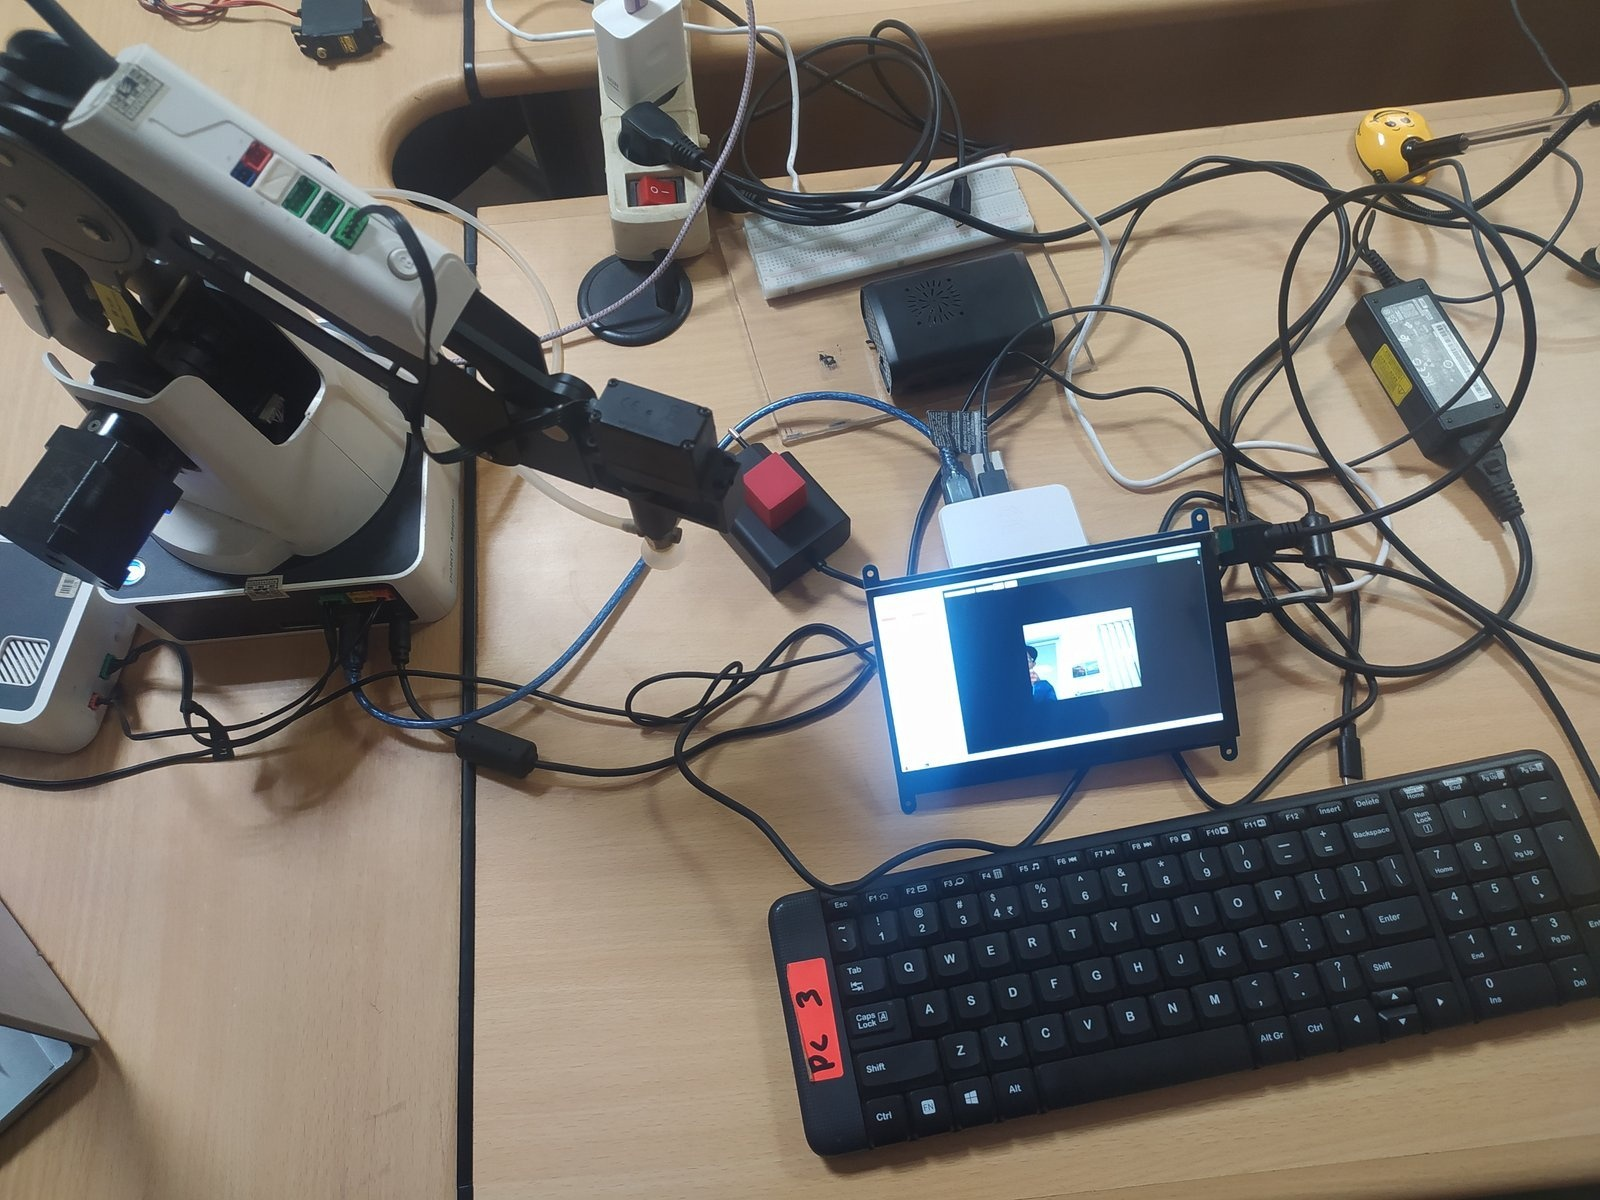
\includegraphics[width=\textwidth]{Gambar/Gambar6_16_stasiun_teleoperasi_dobot2.jpg}
        \caption{Stasiun Kerja Teleoperasi (Sudut 2)}
        \label{fig:app_6_16}
    \end{subfigure}
    \hfill
    \begin{subfigure}[b]{0.48\textwidth}
        \centering
        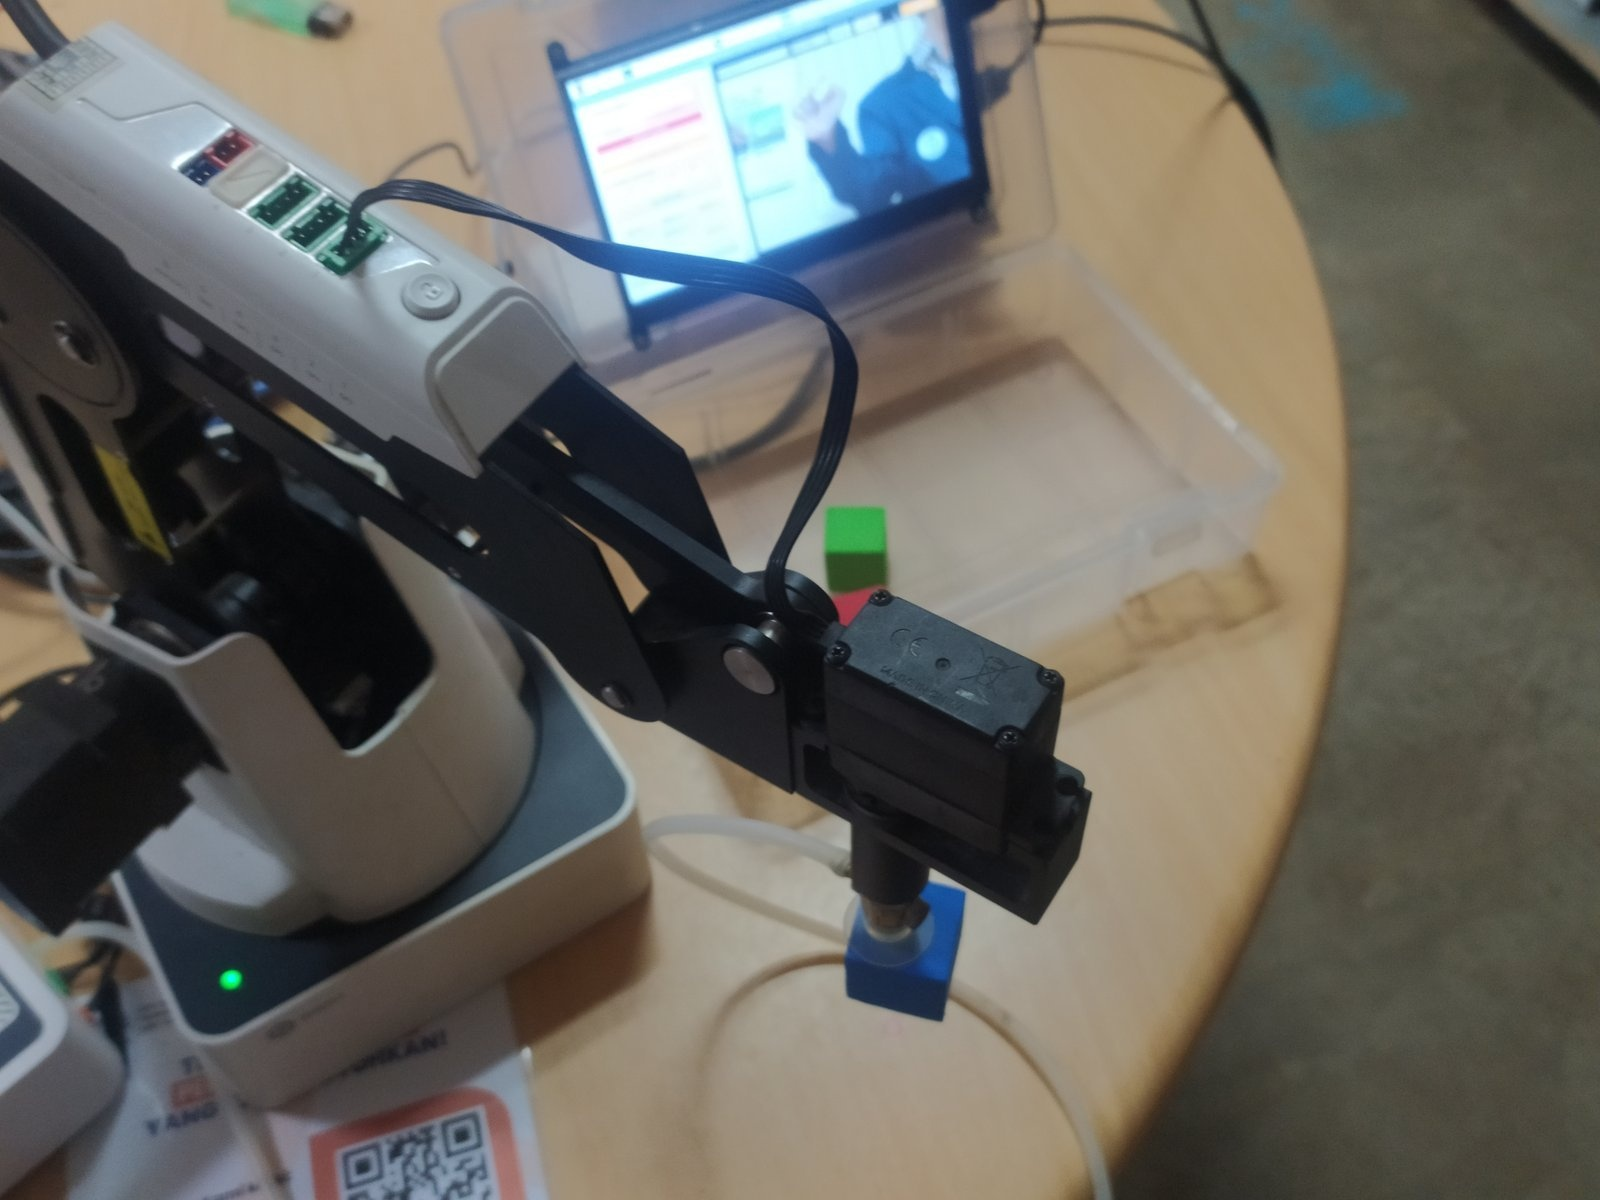
\includegraphics[width=\textwidth]{Gambar/Gambar6_17_manipulator_dobot_suction1.jpg}
        \caption{Manipulator Dobot dan Suction Cup (Sudut 1)}
        \label{fig:app_6_17}
    \end{subfigure}
    \caption{Dokumentasi Manipulator Dobot Magician}
\end{figure}

\begin{figure}[htbp]
    \centering
    \begin{subfigure}[b]{0.48\textwidth}
        \centering
        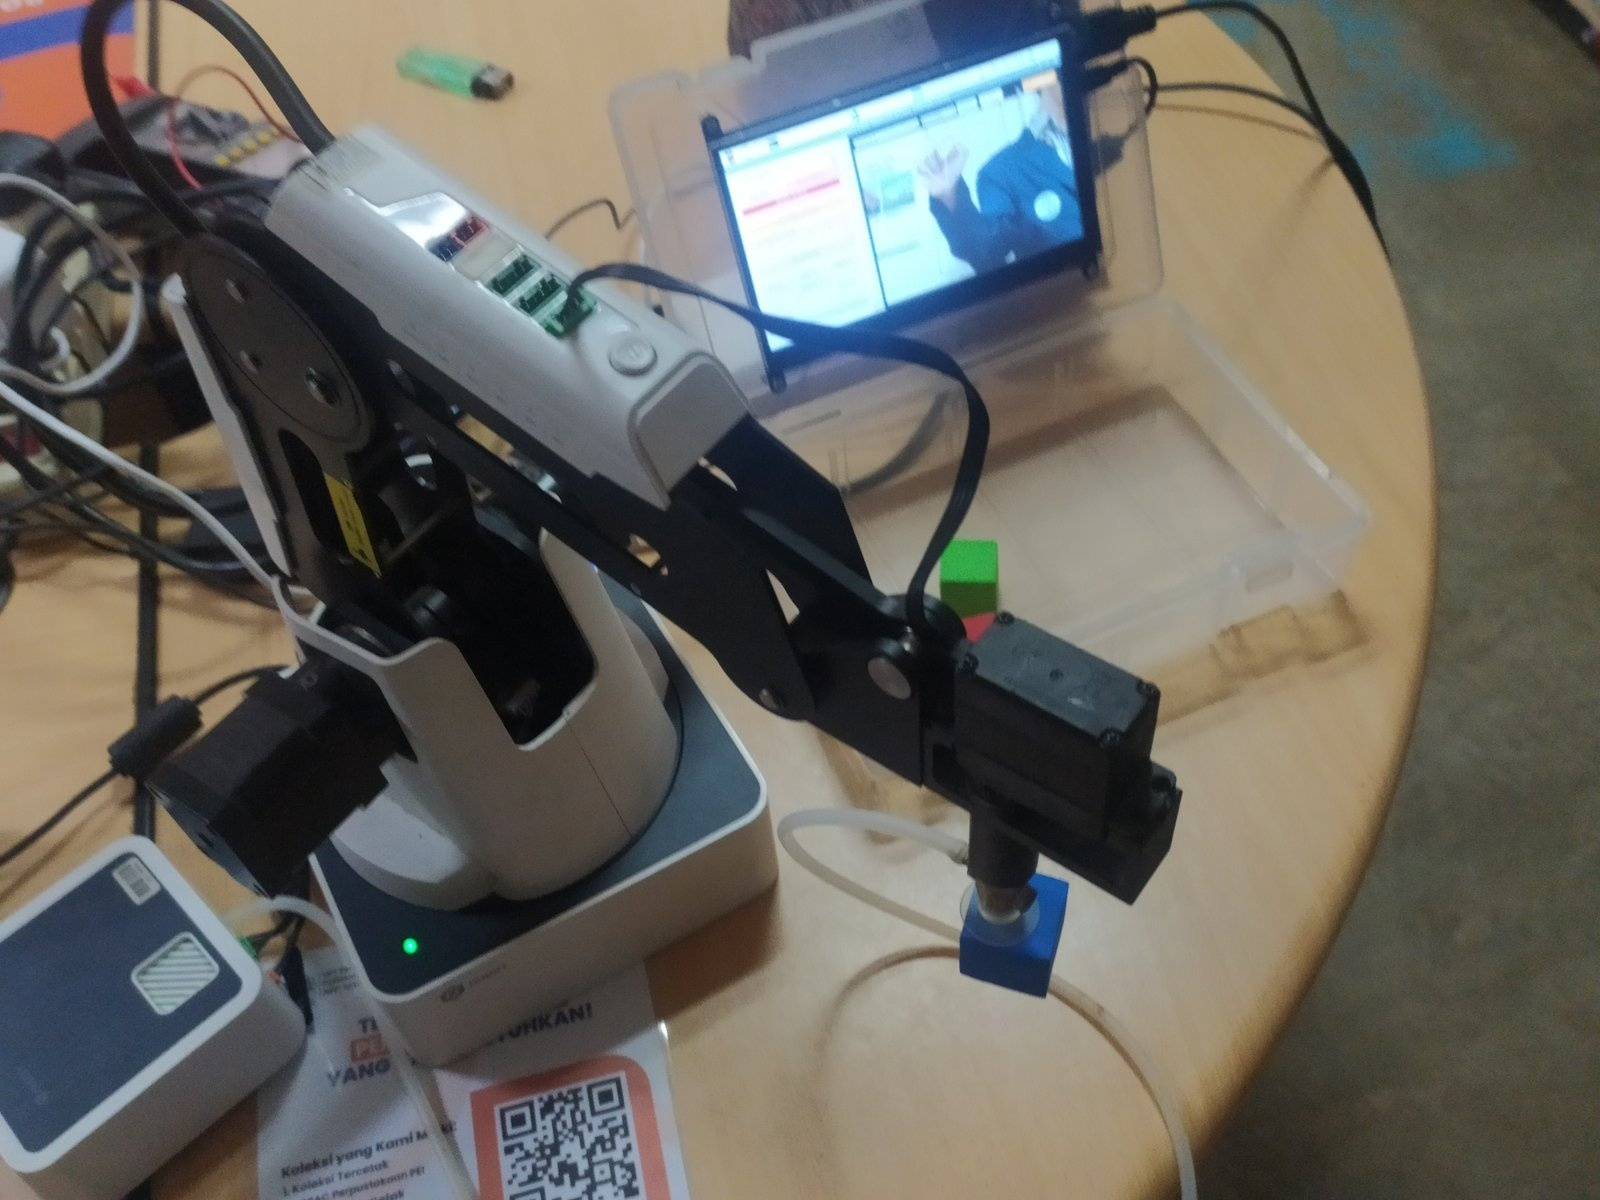
\includegraphics[width=\textwidth]{Gambar/Gambar6_18_manipulator_dobot_suction2.jpg}
        \caption{Manipulator Dobot dan Suction Cup (Sudut 2)}
        \label{fig:app_6_18}
    \end{subfigure}
    \hfill
    \begin{subfigure}[b]{0.48\textwidth}
        \centering
        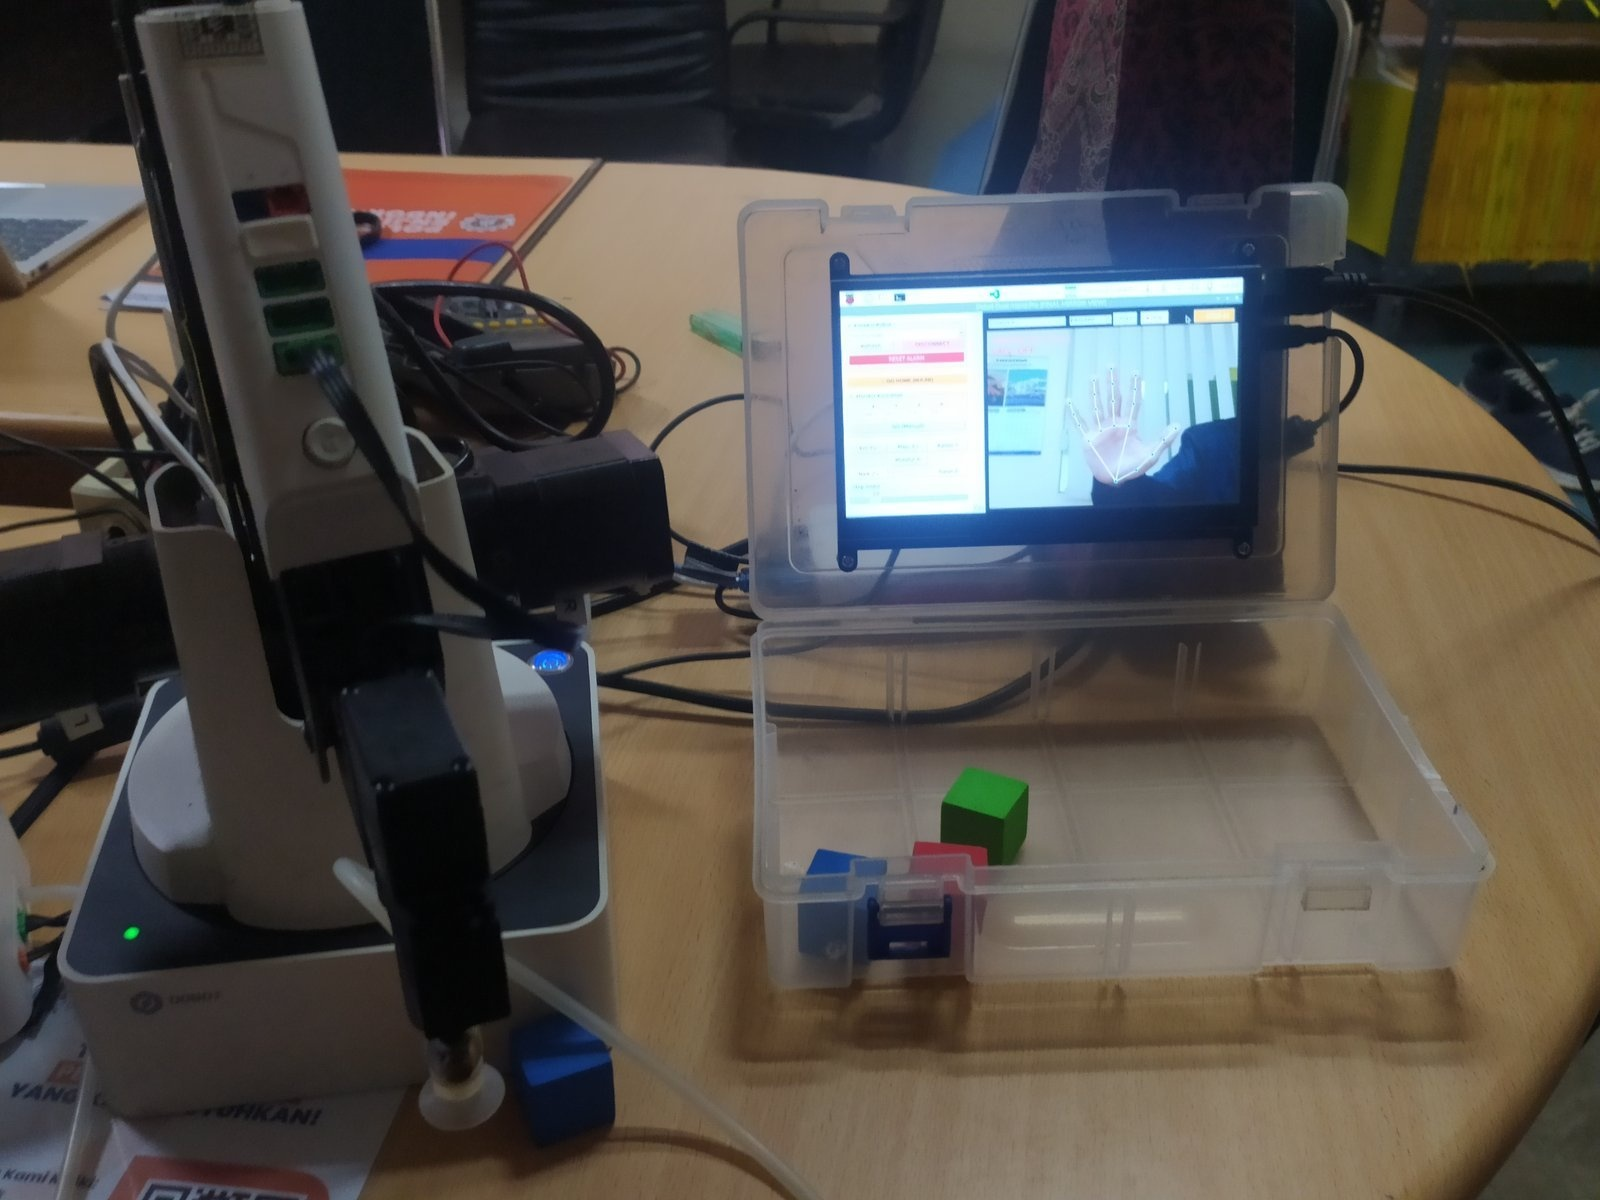
\includegraphics[width=\textwidth]{Gambar/Gambar6_19_manipulator_dobot_suction3.jpg}
        \caption{Manipulator Dobot dan Suction Cup (Sudut 3)}
        \label{fig:app_6_19}
    \end{subfigure}
    \caption{Pengujian Efektor Akhir Suction Cup Dobot Magician}
\end{figure}


\end{document}
